\documentclass[lang=cn,10pt,newtx,thmcnt=section]{vividbook} % 无minted版本!使用这个请务必注释掉48行附近的\input{cha/minteds.tex}


\title{关于自控的那些事}
\subtitle{Automatic Control Theory}


\extrainfo{在没有结束前，总要做很多没有意义的事，这样才可以在未来某一天，用这些无意义的事去堵住那些讨厌的缺口}

\setcounter{tocdepth}{10}

\logo{1.jpg}
\cover{2.jpg}

% 本文档命令
\usepackage{array}
\newcommand{\ccr}[1]{\makecell{{\color{#1}\rule{1cm}{1cm}}}}
% 方便书写的一些命令
\newcommand{\Lcal}{\mathcal{L}}


% 修改标题页的橙色带
\definecolor{customcolor}{RGB}{150, 250, 246}
\colorlet{coverlinecolor}{customcolor}
\usepackage{cprotect}
\usepackage{zhlipsum}
\usepackage{longtable}
\addbibresource[location=local]{reference.bib} % 参考文献，不要删除
\usepackage{animate}
\definecolor{framegolden}{RGB}{0, 174, 247} % 控制外框颜色

\begin{document}

\chapterimage{q2.pdf} 
\maketitle

\frontmatter
\thispagestyle{fancy}
\tableofcontents

\mainmatter

\setcounter{chapter}{-1}
\chapterimage{18.jpg}
% !TEX root = ../../main.tex
\chapter{写在前面的话}

欢迎来到自动控制理论的殿堂！这是自动化专业最重要的专业课之一，虽然说学的内容大部分在后续的生产生活当中都用不到，有些过时了，但毕竟这是前人智慧的结晶！还是很重要的！

本笔记的主要参考书目为哈工大出版社出版的自动控制原理（上）和（下），参考的上课ppt为张宏伟老师、张颖老师、吴爱国老师和许鋆老师的ppt，他们分别教的内容为：
\begin{enumerate}
    \item 张宏伟老师：控制系统的运动分析（时域、频域，离散系统等等）
    \item 张颖老师：控制系统的稳定性分析
    \item 吴爱国老师：控制系统性能指标、频域校正、根轨迹校正
    \item 许鋆老师：PID、离散系统校正、能控能观、状态反馈以及状态观测、非线性控制分析
\end{enumerate}

不过笔者写笔记的思路和这些都有些不一样，本笔记主要分为五个部分：
\begin{enumerate}
    \item 经典控制理论（分析）
    \item 现代控制理论（分析）
    \item 系统的稳定性
    \item 控制系统设计综合
    \item 非线性系统的分析
\end{enumerate}

23级自动化用了三个学期来学习自动控制理论，不过好像后面的又改回了22级及以前的上课方式，采用自控理论A和自控理论B上课，这都无关紧要，学的内容都是大差不差的。祝愿各位哈工深的大三自动化学子们能度过一个愉快的大三生活！

也希望看到这份笔记的友友们如果发现有什么写错或者写漏了的部分可以向笔者提出来，笔者的联系方式为：\textbf{QQ：2745813833}，笔者不保证所有的内容都是对的，毕竟是上了三个学期才写出来的笔记，大家一起把这份笔记做完整做全对！

\begin{marker}
    本笔记中存在超链接，带有超链接的字会标粉，可以直接双击跳转到对应的位置
\end{marker}


\partsimage{cov18.pdf}
\part{经典控制理论}

\chapterimage{9.jpg}
\chapter{控制系统的数学模型}
\section{建立数学模型的方法}
我们通过一下的几种方法建立系统的数学模型：
\begin{enumerate}
    \item 机理分析法(\textbf{白箱模型}):
        根据基本的物理规律、化学规律以及能量守恒定律等，动态系统可以用微分方程描述
    \item 试验法/测试法(\textbf{黑箱模型})：
        通过一些经典信号激励，看系统的响应如何（脉冲响应，阶跃响应.....）
    \item 综合法(\textbf{灰箱模型})：
        一般通过机理分析建立模型的结构，然后通过系统辨识确定模型参数
\end{enumerate}

\section{物理系统的数学模型举例}
\begin{example}
    如图所示为弹簧-质量块-阻尼系统，设外界输入为$F$，滑块输出量为$y$和$v$，则可以列出以下式子：
    \begin{center}
        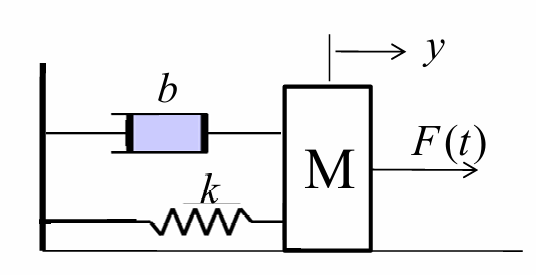
\includegraphics[width=0.3\textwidth]{note/mathmodel/figure/1.png}
    \end{center}

    \begin{equation*}
        \begin{split}
            &M\ddot{y} + ky + b\dot{y} = F(t) \\
            &M\dot{v} + bv + k \int_0^t v(\tau) d\tau = F(t)\\
        \end{split}
    \end{equation*}
\end{example}

\begin{example}
    如图所示为RLC并联电路，设外界输入为$I(t)$ ，电路中输出量为：$i_L$ 和$u_c$ ，则可以列出以下式子：
    \begin{center}
        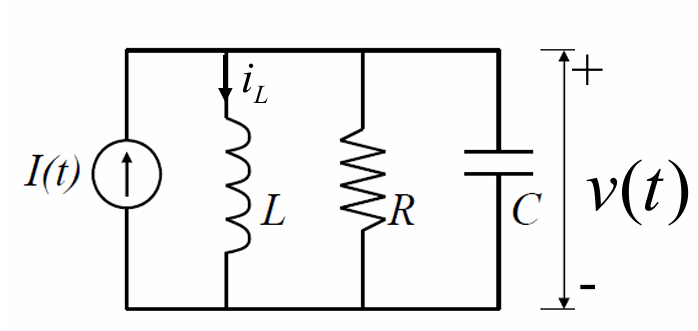
\includegraphics[width = .3\textwidth]{note/mathmodel/figure/2.png}
    \end{center}

    \begin{equation*}
        \begin{split}
            &C\dot{u_c} + \frac{1}{R}u_c + \frac{1}{L} \int_0^t u_c(\tau) d\tau = I(t) \\
            &CL\ddot{i_L} +\frac{L}{R}\dot{i_L} + i_L = I(t) 
        \end{split}
    \end{equation*}

\end{example}

\section{Laplace变换}
\begin{definition}[拉氏变换]
    Laplace变换可以简略定义为如下形式：
    \begin{equation*}
        F(s) = \mathcal{L}[f(t)] = \int_{0^{-}}^\infty f(t) e^{-st} dt 
    \end{equation*}
    当且仅当$f(t) e^{-st}$ 绝对可积 \\
    当然，在物理中可实现信号通常都是可变换的
\end{definition}

\begin{definition}[拉氏逆变换]
    Laplace逆变换可以简略定义为如下形式：
    \begin{equation*}
        f(t) = \mathcal{L}^{-1} [F(s)] = \frac{1}{2\pi j} \int_{\sigma - j \infty} ^{\sigma + j\infty} F(s) e^{st} dt
    \end{equation*}
    当我们掌握留数的知识后，Laplace逆变换可以用下述式子计算：\\
    设$F(s)$ 的极点为：$s_1,s_2,\cdots,s_n$，则：
    \begin{equation*}
        f(t) = \mathcal{L}^{-1} [F(s)] = \Sigma_{i=1}^n Res[F(s)e^{st},s_i]
    \end{equation*}
\end{definition}

\begin{property}[Laplace变换的性质]
    \begin{enumerate}
        \item 线性性：$\Lcal [\alpha f_1(t) + \beta f_2(t)] = \alpha \Lcal[f_1(t)] + \beta \Lcal[f_2(t)] $ 
        \item 时移性：$\Lcal [f(t-\lambda)] = e^{-s\lambda} \Lcal [f(t)]$ 
        \item 时域伸缩性：$\Lcal [f(at)] = \dfrac{1}{a} \Lcal[f(t)](\dfrac{s}{a}) $
        \item 频移性：$\Lcal[e^{-at}f(t)] = \Lcal[f(t)] (s+a)$ 
        \item 微分性：$\Lcal[\dfrac{d}{dt}f(t)] = s\Lcal[f(t)] - f(0^-)$ 
        \item 积分性：$\Lcal [\int_0^t f(\xi) d\xi] = \dfrac{\Lcal[f(t)]}{s}$ 
        \item 时域卷积：$\Lcal [f_1 * f_2] = \Lcal[f_1]\cdot \Lcal[f_2]$ 
        \item 频域卷积：$\Lcal [f_1\cdot f_2]= \dfrac{1}{2\pi j} \Lcal[f_1] * \Lcal[f_2]$
        \item 频域微分：$\Lcal [tf(t)] = -\dfrac{d}{ds}\Lcal[f(t)] $
        \item 初值定理：$\lim_{t\rightarrow 0^+} f(t) = \lim _{s\rightarrow \infty} s\Lcal[f(t)]$
        \item 终值定理：$ \lim_{t\rightarrow \infty} f(t) = \lim_{s\rightarrow 0} s\Lcal[f(t)]$
    \end{enumerate}
\end{property}

\section{传递函数}
\begin{definition}[传递函数]
    在零初始条件下，线性定常系统或元件输出信号的Laplace变换式$Y(s)$与输入信号的Laplace变换式$R(s)$之比为该系统或元件的传递函数。数学表示为：
    \begin{equation*}
        G(s) = \frac{Y(s)}{R(s)} = \frac{b_m s^m + b_{m-1} s^{m-1} + \cdots + b_1 s +b_0}{s^n + a_{n-1} s^{n-1}+\cdots + a_1 s +a_0}
    \end{equation*}
    注：
    \begin{itemize}
        \item 传递函数反映系统零状态响应的传递关系
        \item 传递函数表明了系统数学模型的阶次n，它表征着系统的固有特性（如系统的结构与参数等），与输入的形式无关
        \item 传递函数是研究线性系统动态特性的重要工具
    \end{itemize}

\end{definition}


\subsection{典型环节的传递函数}
\begin{enumerate}
    \item 惯性环节：$G(s) = \dfrac{1}{Ts+1}$ ，$T$为时间常数
    \item 积分环节：$G(s) = \dfrac{1}{Ts}$ ， $T$为时间常数
    \item 震荡环节：$G(s) = \dfrac{\omega_n^2}{s^2 + 2\zeta \omega_n s + \omega_n^2}$ ，$\zeta$ 为阻尼比，$\omega_n$ 为无阻尼自然震荡角频率
    \item 微分环节：$G(s) = T_d s$
    \item 比例环节：$G(s) = K_p$
    \item 时滞/延迟环节：$G(s) = e^{-\tau s}$ 
\end{enumerate}

\subsection{系统方框图模型}
\begin{definition}[方框图]
    系统方框图模型是系统各环节的传递函数功能和信号流向的图解表示，是一种图形化的数学模型，如下图所示：
    \begin{center}
        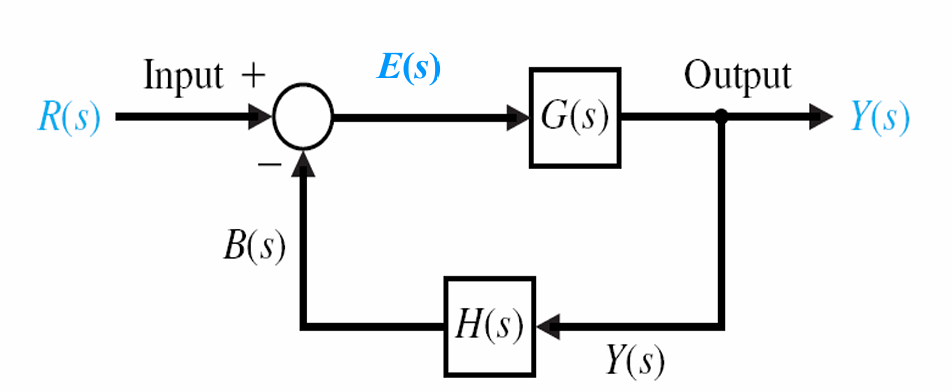
\includegraphics[width=.3\textwidth]{note/mathmodel/figure/3.png}
    \end{center}
    此图为负反馈控制系统的典型结构图，包含以下三个重要参数：
    \begin{enumerate}
        \item 闭环传递函数：$\dfrac{Y(s)}{R(s)}$
        \item 前向传递函数：$\dfrac{Y(s)}{E(s)}$
        \item 开环传递函数：$\dfrac{B(s)}{E(s)}$
    \end{enumerate}
    同时也包含四种基本单元：
    \begin{enumerate}
        \item 信号线
        \item 分支点（引出点、测量点）
        \item 相加点（比较点，综合点）
        \item 方框
    \end{enumerate}
    示例图如下所示：
    \begin{center}
        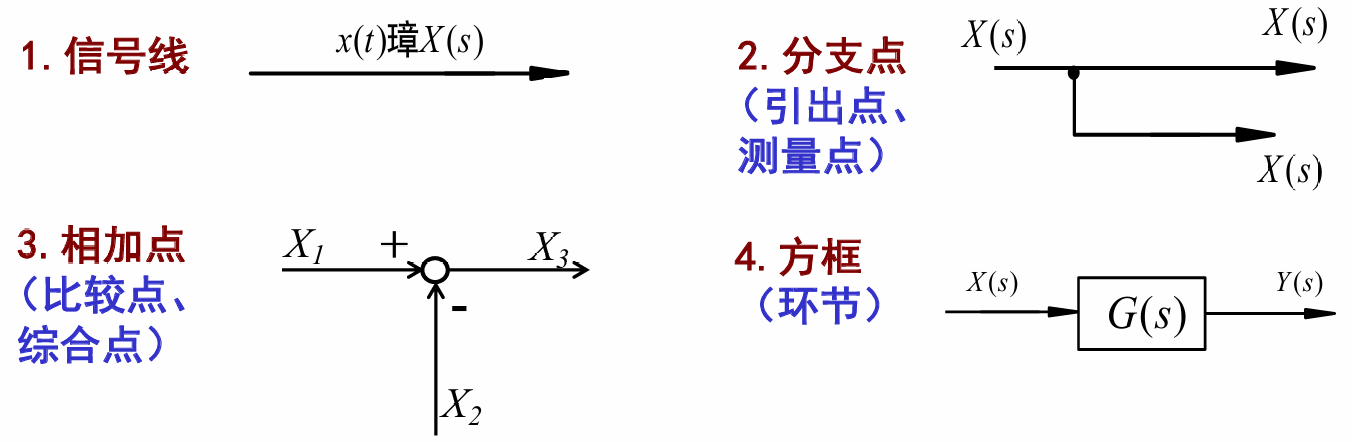
\includegraphics[width = .4\textwidth]{note/mathmodel/figure/4.png}
    \end{center}
\end{definition}

\begin{ascolorbox5}{框图的基本变换}[black!50!white][coltext = black]
    \begin{enumerate}
        \item 合并串联方框：
        \begin{center}
            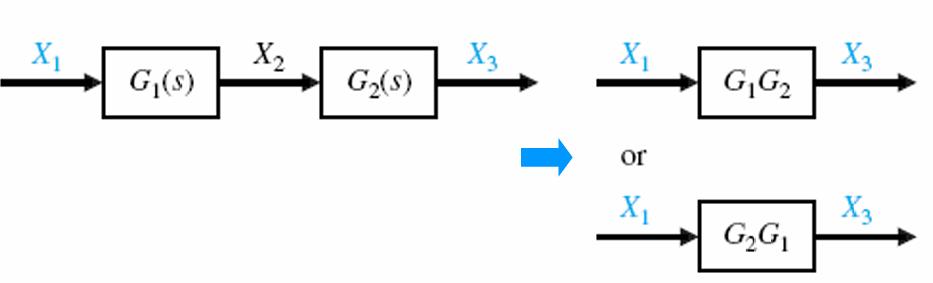
\includegraphics[width = .4\textwidth]{note/mathmodel/figure/5.png}
        \end{center}
        \item 相加点后移：
        \begin{center}
            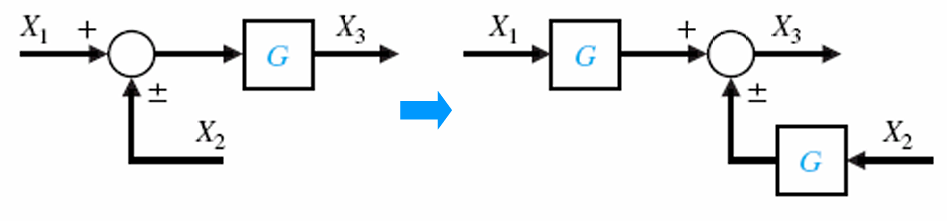
\includegraphics[width = .4\textwidth]{note/mathmodel/figure/6.png}
        \end{center}
        \item 相加点前移：
        \begin{center}
            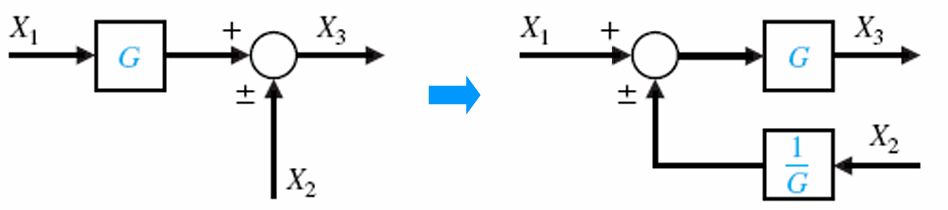
\includegraphics[width = .4\textwidth]{note/mathmodel/figure/7.png}
        \end{center}
        \item 分支点后移：
        \begin{center}
            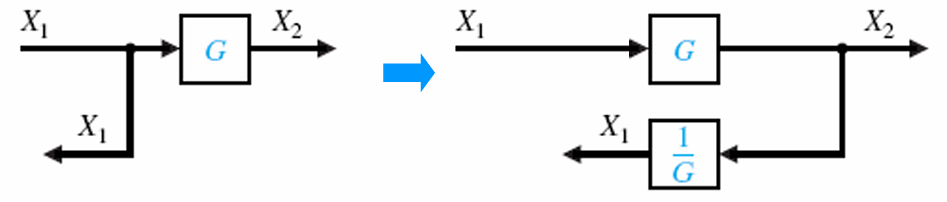
\includegraphics[width = .4\textwidth]{note/mathmodel/figure/8.png}
        \end{center}
        \item 分支点前移：
        \begin{center}
            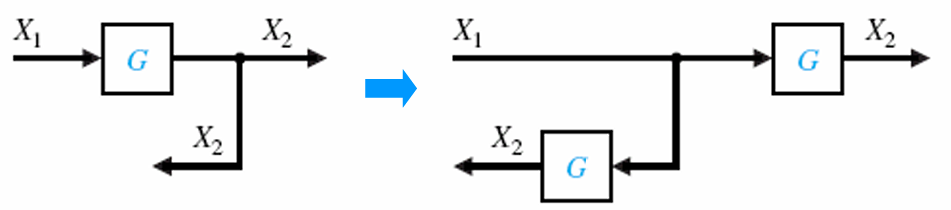
\includegraphics[width = .4\textwidth]{note/mathmodel/figure/9.png}
        \end{center}
        \item 消去反馈通路：
        \begin{center}
            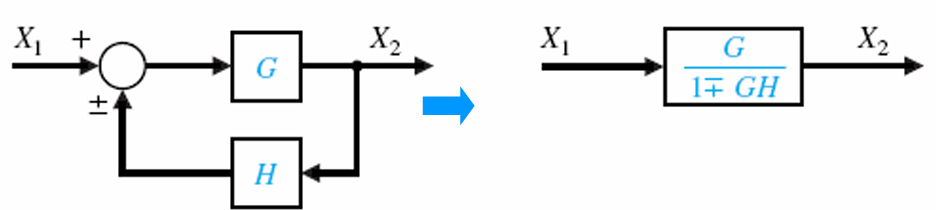
\includegraphics[width = .4\textwidth]{note/mathmodel/figure/10.png}
        \end{center}
        \item 并联方框：
        \begin{center}
            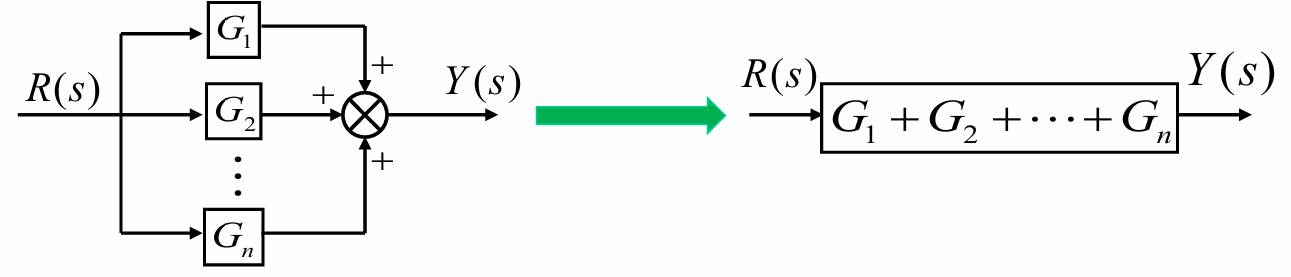
\includegraphics[width = .5\textwidth]{note/mathmodel/figure/11.png}
        \end{center}
        \item 相邻相加点之间的移动：
        \begin{center}
            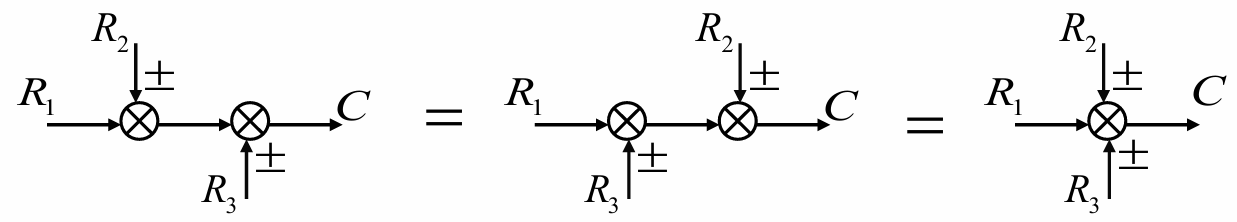
\includegraphics[width = .5\textwidth]{note/mathmodel/figure/12.png}
        \end{center}
        \item 相加点与分支点交换位置：
        \begin{center}
            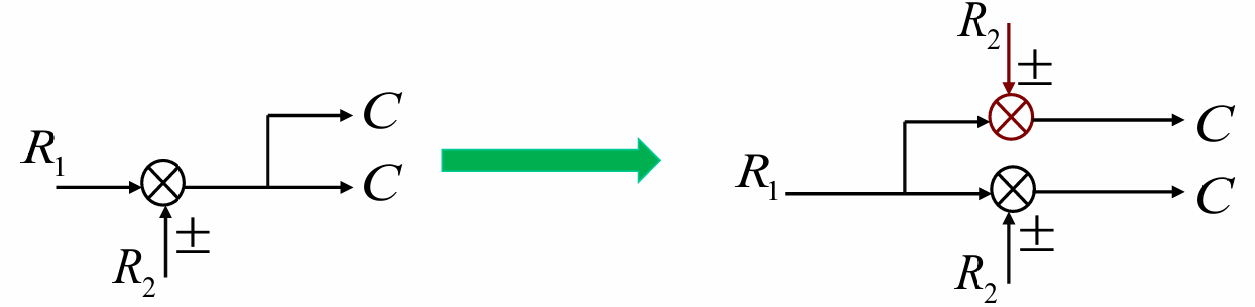
\includegraphics[width = .5\textwidth]{note/mathmodel/figure/13.png}
        \end{center}
    \end{enumerate}
\end{ascolorbox5}

\begin{example}
    化简以下方框图：
    \begin{center}
        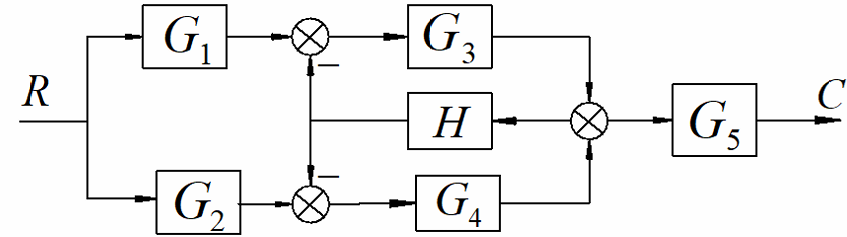
\includegraphics[width = .4\textwidth]{note/mathmodel/figure/14.png}
    \end{center}
    解答如下：
    \begin{itemize}
        \item[(1)] 相加点后移：
        \begin{center}
            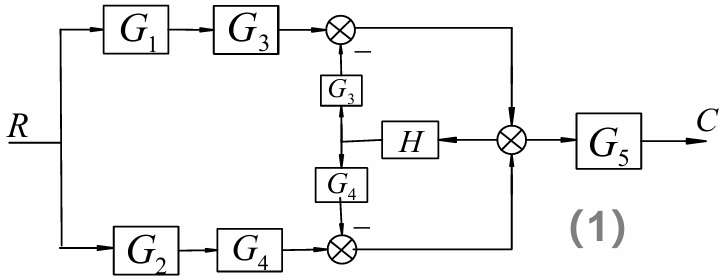
\includegraphics[width = .4\textwidth]{note/mathmodel/figure/15.png}
        \end{center}
        \item[(2)] 分支点前移：
        \begin{center}
            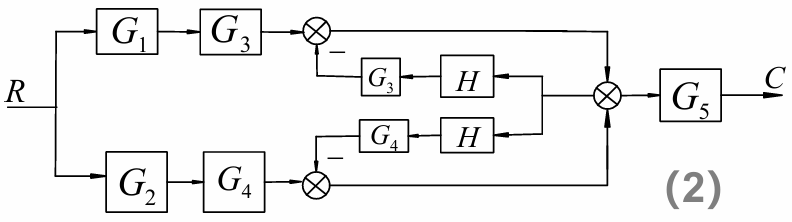
\includegraphics[width = .4\textwidth]{note/mathmodel/figure/16.png}
        \end{center}
        \item[(3)] 合并串联部分：
        \begin{center}
            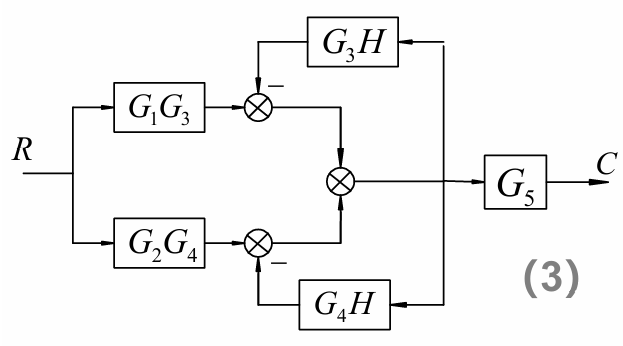
\includegraphics[width = .3\textwidth]{note/mathmodel/figure/17.png}
        \end{center}
        \item[(4)] 拆分相加点：
        \begin{center}
            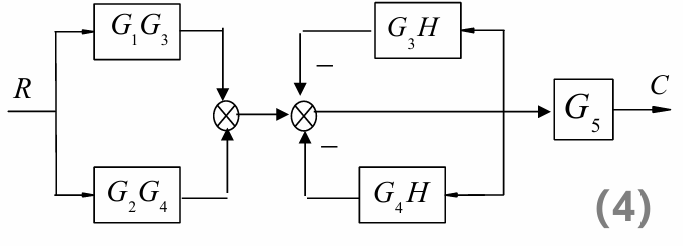
\includegraphics[width = .4\textwidth]{note/mathmodel/figure/18.png}
        \end{center}
        \item[(5)] 合并并联和反馈部分：
        \begin{center}
            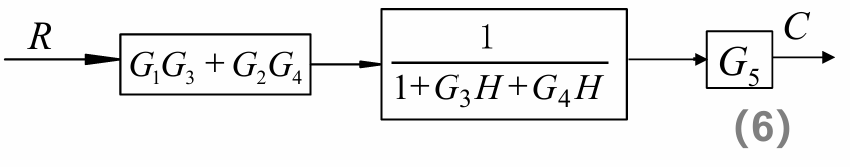
\includegraphics[width = .4\textwidth]{note/mathmodel/figure/19.png}
        \end{center}
        \item[(6)] 合并串联部分：
        \begin{center}
            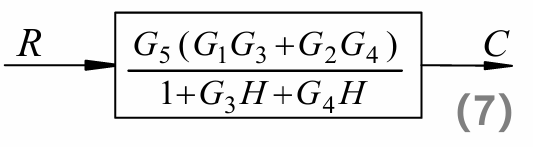
\includegraphics[width = .3\textwidth]{note/mathmodel/figure/20.png}
        \end{center}
    \end{itemize}
\end{example}

\subsection{信号流图}

\begin{definition}[信号流图]
    信号流图是用来表示系统中各变量间相互关系以及信号传递的一种图解方法，包含以下几个部分：
    \begin{enumerate}
        \item 节点（node）：表示系统的变量，用$\circ$表示
        \item 支路（branch）：相当于乘法器，信号流经支路时，被乘以支路增益而变换为另一信号
    \end{enumerate}
    注：
    \begin{itemize}
        \item 信号在支路上只能沿箭头单向传递
        \item 节点具有以下作用：
        \begin{enumerate}
            \item 对所有来自流入支路信号作加法运算
            \item 将流入信号之和传输给所有流出支路
        \end{enumerate}
    \end{itemize}
    一些有关的术语：
    \begin{itemize}
        \item 输入节点（源点）：输入信号对应的节点。只有输出支路，无输入支路
        \item 输出节点（阱点）：输出信号对应的节点，常用传输为1的支路引出。只有输入，没有输出支路
        \item 混合节点：既有输出支路，又有输入支路
        \item 前向通路：当信号从输入节点至输出节点传递时，每个节点只通过一次的通路
        \item 回路：起点和重点是同一节点，而且信号通过每个节点不多于1次的闭合通路
        \item 不接触回路：之间没有公共节点的回路
    \end{itemize}
\end{definition}

\begin{ascolorbox1}{信号流图与方框图之间的转化}[]
    如下图所示为信号流图与方框图之间的转化表：
    \begin{center}
        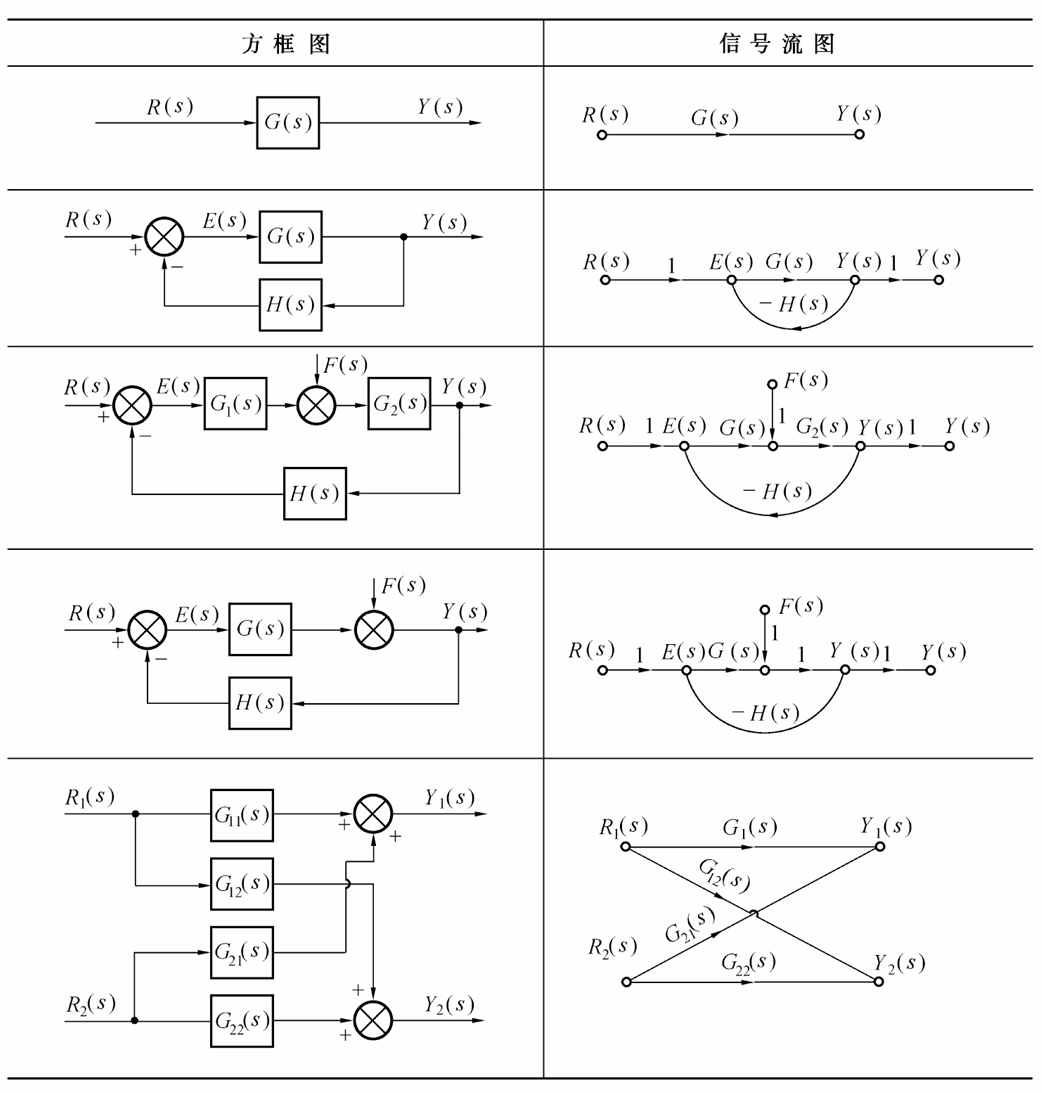
\includegraphics[width = .5\textwidth]{note/mathmodel/figure/21.png}
    \end{center}
\end{ascolorbox1}

\subsection{梅森公式(Mason's formula)}

\begin{definition}
    Mason 公式由以下数学式子给出：
    \begin{equation*}
        P = \frac{1}{\Delta} \Sigma_{k=1}^n P_k \Delta_k
    \end{equation*}
    其中：
    \begin{itemize}
        \item $P$ ：总增益
        \item $P_k$：第k条前向通路的通路增益
        \item $\Delta = 1-\Sigma_{l_1} L_1 + \Sigma_{l_1 l_2} L_1 L_2 -\Sigma_{l_1 l_2 l_3} L_1 L_2 L_3 \cdots +(-1)^n \Sigma_{l_1 l_2 \cdots l_n} L_1 L_2 \cdots L_n \cdots$ 为系统结构图的特征式
        \item $\Sigma_{l_1 l_2 \cdots l_k} L_1 L_2 \cdots L_k$ 为每k个互不接触回路增益乘积之和 ($1\leq k \leq$ 最大回路数)
        \item $\Delta_k$：在特征式中除去与第k条前向通路相接触的回路后的特征式，称为第k条前向通路特征式的余子式
    \end{itemize}
\end{definition}

\begin{example}
    用Mason 增益公式求出以下系统方框图中的传递函数：
    \begin{center}
        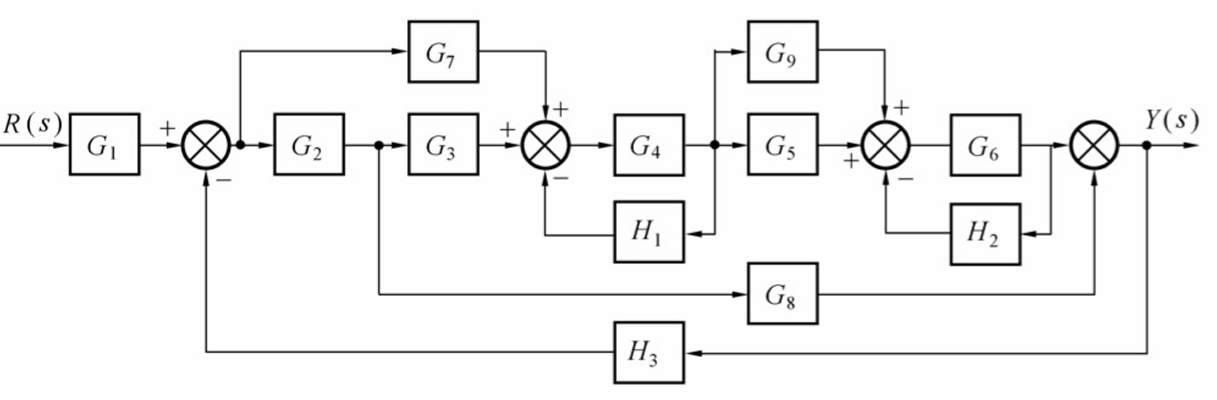
\includegraphics[width=.5\textwidth]{note/mathmodel/figure/22.png}
    \end{center}
    解答如下：
    \begin{itemize}
        \item[(1)] 图中回路增益分别为：
        \begin{equation*}
            \begin{split}
                L_1 = &-G_4 H_1 \\
                L_2 = &-G_6 H_2 \\
                L_3 = &-G_2 G_3 G_4 G_5 G_6 H_3 \\
                L_4 = &-G_2 G_3 G_4 G_9 G_6 H_3 \\
                L_5 = & -G_7 G_4 G_5 G_6 H_3 \\
                L_6 = & -G_7 G_4 G_9 G_6 H_3 \\
                L_7 = & -G_2 G_8 H_3 \\
            \end{split}
        \end{equation*}
        \item[(2)] 每两个互不接触回路增益乘积：
        \begin{equation*}
            \begin{split}
                L_1 L_2 = &G_4 G_6 H_1 H_2 \\
                L_1 L_7 = & G_2 G_4 G_8 H_1 H_3 \\
                L_2 L_7 = & G_2 G_6 G_8 H_2 H_3 \\
            \end{split}
        \end{equation*}
        \item[(3)] 每三个互不接触回路乘积：
        \begin{equation*}
            L_1 L_2 L_7 = -G_2 G_4 G_6 G_8 H_1 H_2 H_3
        \end{equation*}
        \item[(4)] 方框图特征式：
        \begin{equation*}
            \begin{split}
                \Delta =& 1-\Sigma_{i=1}^7 L_i +L_1 L_2 +L_1 L_7 +L_2 L_7-L_1 L_2 L_7\\
                =& 1+G_4 H_1+G_6 H_2+G_2 G_3 G_4 G_5 G_6 H_3+G_2 G_3 G_4 G_9 G_6 H_3+G_7 G_4 G_5 G_6 H_3+G_7 G_4 G_9 G_6 H_3+G_2 G_8 H_3 \\
                &+G_4 G_6 H_1 H_2+G_2 G_4 G_8 H_1 H_3+G_2 G_6 G_8 H_2 H_3
            \end{split}
        \end{equation*}
        \item[(5)] 前向通路增益及其余子式：
        \begin{equation*}
            \begin{split}
                P_1 = G_1 G_2 G_3 G_4 G_5 G_6 \quad &\Delta_1 = 1 \\
                P_2 = G_1 G_2 G_8 \quad &\Delta_2 = 1 + G_4 H_1 + G_6 H_2 +G_4 G_6 H_1 H_2 \\
                P_3 = G_1 G_7 G_4 G_5 G_6 \quad & \Delta_3 = 1 \\
                P_4 = G_1 G_2 G_3 G_4 G_9 G_6 \quad &\Delta_4 = 1 \\
                P_5 = G_1 G_7 G_4 G_9 G_6 \quad &\Delta_5 = 1 \\
            \end{split}
        \end{equation*}
        \item[(6)] 由Mason 增益公式$P = \dfrac{1}{\Delta} \Sigma_{k=1}^3 P_k \Delta_k$ 即可得出答案（答案过长不方便写在此处）
    \end{itemize}
\end{example}



\chapterimage{10.jpg}
\chapter{控制系统的时域分析与综合}
\section{典型输入信号}
\begin{definition}[单位阶跃函数]
    单位阶跃函数的表达式如下：
    \begin{equation*}
        r(t) = \begin{cases}
            1 \quad & t\geq 0 \\
            0 \quad & t<0
        \end{cases}
    \end{equation*}
    示意图如图：
    \begin{center}
        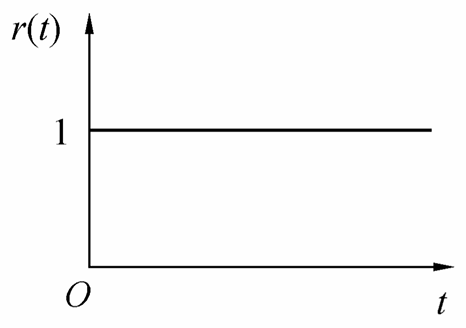
\includegraphics[width=.2\textwidth]{note/time-domain analysis/figure/1.png}
    \end{center}
    Laplace变换后：$R(s) = \dfrac{1}{s}$
\end{definition}

\begin{definition}[单位斜坡函数]
    单位斜坡函数的表达式如下：
    \begin{equation*}
        r(t) = \begin{cases}
            t \quad & t>0 \\
            0 \quad & t<0
        \end{cases}
    \end{equation*}
    示意图如图：
    \begin{center}
        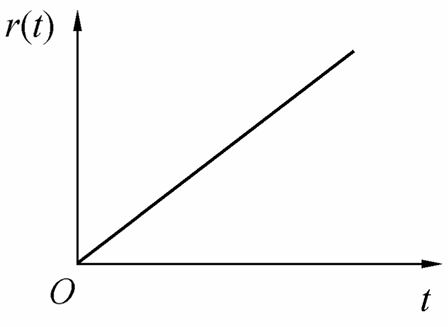
\includegraphics[width=.2\textwidth]{note/time-domain analysis/figure/2.png}
    \end{center}
    Laplace变换后：$R(s) = \dfrac{1}{s^2}$
\end{definition}

\begin{definition}[单位加速度函数]
    单位加速度函数的表达式如下：
    \begin{equation*}
        r(t) = \begin{cases}
            \frac{1}{2}t^2 \quad & t\geq 0 \\
            0 \quad & t<0
        \end{cases}
    \end{equation*}
    示意图如图：
    \begin{center}
        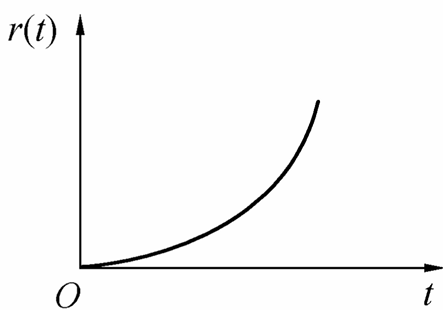
\includegraphics[width=.2\textwidth]{note/time-domain analysis/figure/3.png}
    \end{center}
    Laplace变换后：$R(s) = \dfrac{1}{s^3}$
\end{definition}

\begin{definition}[单位冲激函数]
    单位冲激函数的表达式如下：
    \begin{equation*}
        \begin{split}
            &\delta(t) = \begin{cases}
                \infty \quad & t\neq 0 \\
                0 \quad & t=0
            \end{cases}\\
            &\int_{-\infty}^{\infty} \delta(t) dt = 1
        \end{split}
    \end{equation*}
    Laplace变换后：$R(s) = 1$
\end{definition}

\begin{definition}[正弦信号]
    正弦信号的表达式如下：
    \begin{equation*}
        r(t) = A \sin (\omega t + \varphi)
    \end{equation*}
    Laplace变换后：$R(s) = A e^{\frac{\varphi}{\omega} s} \dfrac{\omega}{s^2+\omega^2}$
\end{definition}

\begin{definition}[动态性能指标]
    在时域分析中我们主要关注以下几个动态性能指标：
    \begin{enumerate}
        \item 延迟时间$t_d$：系统响应从0第一次上升到稳态值的50\%所需要的时间
        \item 上升时间$t_r$：
        \begin{itemize}
            \item 有振荡系统时：系统响应从0第一次上升到稳态值所需的时间
            \item 无振荡系统时：系统响应从稳态值的10\%上升到90\%所需的时间
        \end{itemize}
        \item 峰值时间$t_p$：系统响应第一次达到最大峰值所需要的时间
        \item 超调量$\sigma$：系统响应超出稳态值的最大偏移量（常以百分比表示），$\sigma\% \triangleq \dfrac{y(t_p) - y(\infty)}{y(\infty)}$
        \item 调节时间$t_s$：系统响应与稳态值之差达到并维持误差$\pm\delta$所需要的最短时间，即：$\left\lvert\dfrac{y(t_p) - y(\infty)}{y(\infty)} \right\rvert \leq \delta ,t\geq t_s $
        \item 震荡次数$N$：调节时间$t_s$内，$y(t)$偏离$y(\infty)$的振荡次数
    \end{enumerate}
\end{definition}

\section{一阶系统的时域分析}
\subsection{一阶系统的单位阶跃响应}
\begin{enumerate}
    \item 输入量：$r(t) = 1$ ，$R(s) = \dfrac{1}{s}$
    \item 输出量：$Y(s) = G(s)R(s) = \dfrac{1} {(Ts+1)s}$ ， $y(t) = 1- e^{-\frac{t}{T}}$
    \item 延迟时间：$t_d = 0.69T$
    \item 上升时间：$t_r = 2.2T$ 
    \item 调节时间：$t_s = 3T \,(\Delta = 5\%)$
\end{enumerate}

\begin{ascolorbox3}{一阶系统单位阶跃响应特点}[color = red!40!yellow][coltitle=blue!50!green]
    \begin{enumerate}
        \item 系统输出为初值为0，终值为1的单调连续上升过程。
        \item 响应曲线终值为1，稳态误差为0。
        \item 响应曲线在$T=0$时斜率最大，为$\dfrac{1}{T}$
        \item 动态性能与常数$T$有关，当$t=T$时，响应曲线上升到稳态值的63.2\%
    \end{enumerate}
\end{ascolorbox3}

\subsection{一阶系统的单位冲激响应}
\begin{enumerate}
    \item 输入量：$r(t) = \delta(t)$，$R(s) = 1$ 
    \item 输出量：$Y(s) = \dfrac{1}{Ts+1}$，$y(t) = \dfrac{1}{T} e^{-\frac{t}{T}}$
\end{enumerate}

\begin{ascolorbox3}{一阶系统单位冲激响应特点}[color = green!40!blue][coltitle = red!60!yellow]
    \begin{enumerate}
        \item 系统输出时单调连续下降的指数曲线
        \item 响应曲线的终值为0，稳态误差为0
        \item 动态性能与常数$T$有关，$y(0) = \dfrac{1}{T}\quad y(T) = 0.368\dfrac{1}{T}\quad y(\infty) = 0$
        \item 和传递函数一样，单位冲激响应可以反映系统全部性质，单位冲激响应与传递函数互为Laplace变换对
    \end{enumerate}
\end{ascolorbox3}

\subsection{一阶系统的单位斜坡响应}
\begin{enumerate}
    \item 输入$r(t) = t$，$R(s) = \dfrac{1}{s^2}$
    \item 输出$Y(s) = \dfrac{1}{s^2(Ts+1)}$，$y(t) = t-T(1-e^{-\frac{t}{T}})$
    \item 误差量：$e(t) = T(1-e^{-\frac{t}{T}})$，$e(\infty) = T$
\end{enumerate}

\section{二阶系统的时域分析}
\begin{definition}[二阶系统的标准形式]
    标准形式的二阶系统满足以下式子：
    \begin{enumerate}
        \item 开环传递函数：$G(s) = \dfrac{\omega_n^2}{s(s+2\zeta \omega)}$
        \item 闭环传递函数：$\varPhi(s) = \dfrac{\omega_n^2}{s^2 + 2\zeta \omega_n s + \omega_n^2}$
        \item 闭环极点：$s_{1,2} = -\zeta \omega_n \pm \omega_n \sqrt{\zeta^2 -1}$
    \end{enumerate}
    其中$\omega_n$为无阻尼振荡频率，$\zeta$为阻尼比
\end{definition}

\subsection{二阶系统的单位阶跃响应}
根据$\zeta$的取值我们可以把响应分为四种情况：欠阻尼、零阻尼、过阻尼、临界阻尼和负阻尼

\subsubsection{欠阻尼情况$(0<\zeta<1)$}
欠阻尼条件下$\zeta$满足$0<\zeta<1$，定义阻尼振荡频率：$\omega_d = \omega_n\sqrt{1-\zeta^2}$，则有：
\begin{equation*}
    \begin{split}
        Y(s) &= \frac{\omega_n^2}{s^2 + 2\zeta\omega_n s +\omega_n^2}\cdot\frac{1}{s} = \frac{1}{s} - \frac{s+\zeta \omega_n}{(s+\zeta \omega_n)^2+\omega_d^2}-\frac{\zeta\omega_n}{(s+\zeta \omega_n)^2+\omega_d^2} \\
        y(t) &= \Lcal^{-1}[Y(s)] = 1-e^{-\zeta \omega_n t}(\cos \omega_d t +\frac{\zeta}{\sqrt{1-\zeta^2}} \sin \omega_d t) = 1- e^{-\zeta \omega_n t}\frac{1}{\sqrt{1-\zeta^2}}\sin (\omega_d t +\theta)
    \end{split}
\end{equation*}

\begin{ascolorbox9}{欠阻尼的动态过程指标}
    \begin{enumerate}
        \item 上升时间$t_r = \dfrac{\pi - \theta}{\omega_n \sqrt{1-\zeta^2}}$
        \item 峰值时间$t_p = \dfrac{\pi}{\omega_d} = \dfrac{\pi}{\omega_n \sqrt{1-\zeta^2}}$
        \item 超调量$\sigma_p = e^{-\frac{\zeta}{\sqrt{1-\zeta^2}}\pi} \times 100\%$
        \item 调整时间$t_s = \dfrac{1}{\zeta \omega_n} \ln\dfrac{1}{\Delta \sqrt{1-\zeta^2}}\text{(近似解)} = 
        \begin{cases}
            \dfrac{4}{\zeta \omega_n} & \quad \Delta = 0.02 \\
            \dfrac{3}{\zeta\omega_n} & \quad  \Delta = 0.05 
        \end{cases}\text{（数值解）}$
        \item 振荡次数$N = \begin{cases}
            \dfrac{2\sqrt{1-\zeta^2}}{\pi \zeta} & \quad \Delta = 0.02 \\
            \dfrac{1.5\sqrt{1-\zeta^2}}{\pi \zeta} & \quad \Delta = 0.05
        \end{cases}$
    \end{enumerate}
\end{ascolorbox9}

\begin{example}
    已知二阶系统的闭环传递函数为：
    \begin{equation*}
        \varPhi(s) = \frac{\omega_n^2}{s^2 + 2\zeta \omega_n s +\omega_n^2}
    \end{equation*}
    其中$\zeta = 0.6 \quad \omega_n = 5$rad/s。试计算该系统的单位阶跃响应的特征量$t_r,t_p,t_s,\sigma_p$和$N$\\
    \textbf{解}: 由已知可得：
    \begin{equation*}
        \begin{split}
            t_r/\mathrm{s} &= \frac{\pi-\theta}{\omega_n\sqrt{1-\zeta^2}} = 0.55 \\
            t_p/\mathrm{s} &= \frac{\pi}{\omega_n\sqrt{1-\zeta^2}} = 0.785 \\
            \sigma_p &= e^{-\frac{\zeta \pi}{\sqrt{1-\zeta^2}}}\times 100\% = 9.5\% \\
            t_s/\mathrm{s} &= \frac{4}{\zeta \omega_n} \approx 1.4 \quad \Delta = 0.02\\
            t_s/\mathrm{s} &= \frac{3}{\zeta \omega_n} \approx 1.1 \quad \Delta = 0.05 \\
            N/\text{次} &= \frac{2\sqrt{1-\zeta^2}}{\pi \zeta} \approx 1
        \end{split}
    \end{equation*}
\end{example}

\subsubsection{零阻尼情况$(\zeta=0)$}
在欠阻尼条件下令$\zeta \rightarrow 0$即可得到：
\begin{equation*}
    y(t) = 1- \cos \omega_n t
\end{equation*}

\subsubsection{临界阻尼情况$(\zeta = 1)$}
由已知可以得到系统的响应为：
\begin{equation*}
    \begin{split}
        Y(s) &= \frac{\omega_n^2}{(s+\omega_n)^2}\cdot \frac{1}{s} = \frac{1}{s}-\frac{\omega_n}{(s+\omega_n)^2}-\frac{1}{s+\omega_n}\\
        y(t) &= 1-e^{-\omega_n t}(1+\omega_n t)
    \end{split}
\end{equation*}

\subsubsection{过阻尼情况$(\zeta>1)$}
由已知可以得到系统的响应为：
\begin{equation*}
    \begin{split}
        Y(s) &= \frac{\omega_n^2}{(s+\zeta\omega_n + \omega_n\sqrt{\zeta^2 - 1})(s+\zeta\omega_n - \omega_n\sqrt{\zeta^2 - 1})} \cdot \frac{1}{s} \\
        y(t) &= 1- \frac{1}{2\sqrt{\zeta - 1}(\zeta - \sqrt{\zeta^2 -1})} e^{-(\zeta - \sqrt{\zeta - 1})\omega_n t} + \frac{1}{2\sqrt{\zeta^2 - 1}(\zeta + \sqrt{\zeta ^2 -1})} e^{-(\zeta + \sqrt{\zeta^2 - 1})\omega_n t}
    \end{split}
\end{equation*}

\subsubsection{负阻尼$(-1<\zeta<0)$}
由已知可以得到系统的响应为：
\begin{equation*}
    y(t) = 1 - \frac{e^{-\zeta \omega_n t}}{\sqrt{1-\zeta^2}}\sin (\omega_d t +\theta)
\end{equation*}\\
其中$\omega_d = \omega_n \sqrt{1-\zeta^2} \quad \theta = \arctan \dfrac{\sqrt{1-\zeta^2}}{\zeta}<0$ \\

下图可以同时表现出五种阶跃响应状态之间的变化情况：
\begin{center}
    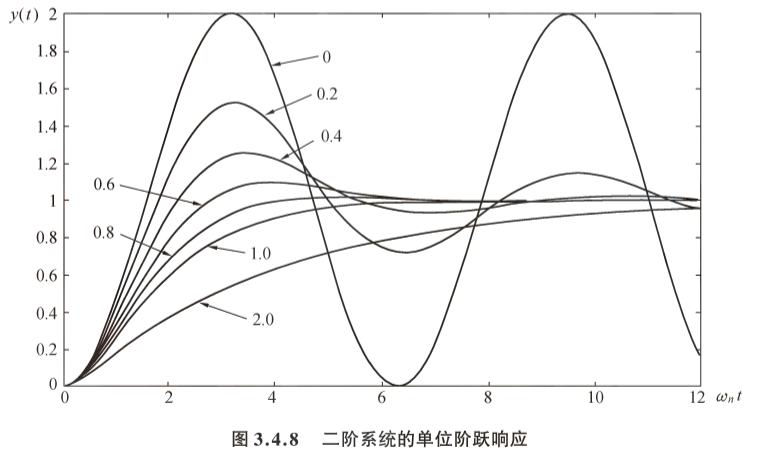
\includegraphics[width = .4\textwidth]{note/time-domain analysis/figure/4.png}
\end{center}

\subsection{二阶系统的单位冲激响应}
由已知其输出就等于系统的闭环传递函数：$Y(s) = \dfrac{\omega_n^2}{s^2 +2\zeta \omega_n s+\omega_n^2}$\\

对此式做Laplace反变换即可得到下列各种情况下的二阶系统单位冲激响应：
\begin{enumerate}
    \item 无阻尼$(\zeta = 0)$：$k(t) = \omega_n \sin\omega_n t \quad (t\geq 0)$ 
    \item 欠阻尼$(0<\zeta<1)$：$k(t) = \dfrac{\omega_n}{\sqrt{1-\zeta^2}}\sin \omega_d t \quad (t\geq 0 )$
    \item 临界阻尼$(\zeta = 1)$：$k(t) =  \omega_n^2 t e^{-\omega t} \quad(t\geq 0)$
    \item 过阻尼$(\zeta > 1)$：$k(t) = \dfrac{\omega_n}{2\sqrt{\zeta^2-1}}[e^{-(\zeta - \sqrt{\zeta^2 - 1})\omega_n t}-e^{-(\zeta + \sqrt{\zeta^2 - 1})\omega_n t}] \quad (t\geq 0)$ 
\end{enumerate}

用一个图可以一起表示上述四个情况的图像：
\begin{center}
    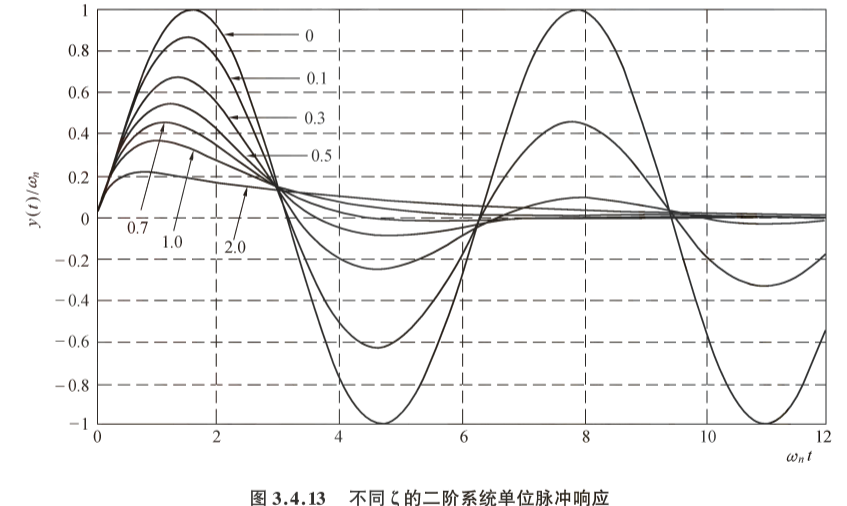
\includegraphics[width = .5\textwidth]{note/time-domain analysis/figure/5.png}
\end{center}

单独讨论二阶欠阻尼系统的单位冲激响应，如图所示：
\begin{center}
    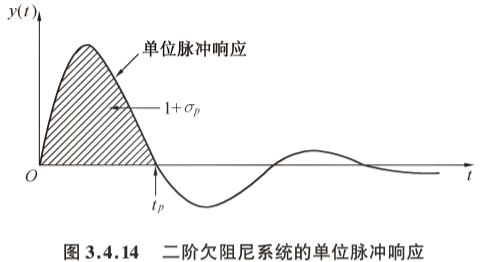
\includegraphics[width = .3\textwidth]{note/time-domain analysis/figure/6.png}
\end{center}
由于$\int_0^{t_p} k(t) dt = y(t_p) = 1+\sigma_p$，
所以上图中阴影部分面积为$1+\sigma_p$

\subsection{二阶系统的单位斜坡响应}
由已知可得系统在复频域的输出为：
\begin{equation*}
    Y(s) = \frac{\omega_n^2}{s^2+2\zeta \omega_n s+\omega_n^2}\cdot \frac{1}{s^2} = \frac{1}{s^2}-\frac{2\zeta/\omega_n}{s} + \frac{2\zeta(s+\zeta\omega_n)/\omega_n+(2\zeta^2 -1)}{s^2+2\zeta \omega_n s +\omega_n^2}
\end{equation*}

对此式做Laplace反变换即可得到下列各种情况下的二阶系统单位斜坡响应：
\begin{enumerate}
    \item 欠阻尼$(0<\zeta<1)$：$y(t) = t-\dfrac{2\zeta}{\omega_n} + \dfrac{1}{\omega_n\sqrt{1-\zeta^2}} e^{-\zeta\omega_n t}\sin (\omega_d t + \arctan\dfrac{2\zeta\sqrt{1-\zeta^2}}{2\zeta^2 - 1})$

    \item 临界阻尼$(\zeta =1)$：$y(t) = t - \frac{2}{\omega_n} + \frac{2}{\omega_n}e^{-\omega_n t}(1 + \dfrac{\omega_n}{2} t)$

    \item 过阻尼$(\zeta >1)$：$y(t) = t - \dfrac{2\zeta}{\omega_n} - \dfrac{2\zeta^2 - 1 - 2\zeta\sqrt{\zeta^2 - 1}}{2\omega_n \sqrt{\zeta^2 - 1}}e^{-(\zeta - \sqrt{\zeta^2 - 1})\omega_n t} + \dfrac{2\zeta^2 - 1 +2\zeta \sqrt{\zeta^2 - 1}}{2\omega_n \sqrt{\zeta^2 -1}}e^{-(\zeta - \sqrt{\zeta^2-1})\omega_n t}$
\end{enumerate}

\section{高阶系统的时域分析}
\subsection{高阶系统的阶跃响应}
高阶系统的闭环传递函数的一般形式是：
\begin{equation*}
    \varPhi (s) = \frac{Y(s)}{R(s)} = \frac{b_m s^m + b_{m-1} s^{m-1} + \cdots + b_1 s +b_0}{a_n s^n + a_{n-1} s^{n-1} + \cdots + a_1 s +a_0} = \frac{k\prod_{i=1}^m(s-z_i)}{\prod_{j=1}^n(s-s_j)}\text{(零极点形式)}
\end{equation*}

对上式运用Laplace反变换（参照定义1.3.2中Laplace逆变换的留数算法）

\subsection{闭环主导极点}
\begin{definition}[闭环主导极点]
    在高阶系统中存在很多极点，将对系统动态过程起主导作用的闭环极点，称为闭环主导极点
\end{definition}

寻找闭环主导极点的一种方法（不完全能用）：若在闭环极点中存在一对共轭复数极点（或一个实数极点）距离虚轴最近，其他极点到虚轴的距离都是它的5倍以上，并且距离虚轴较近处又没有单独的闭环零点，则这对或这个距离虚轴最近的极点称为高阶系统的主导极点

\section{改善控制系统动态性能的方法}
\subsection{速度反馈}
如图所示为带有速度反馈的二阶系统：
\begin{center}
    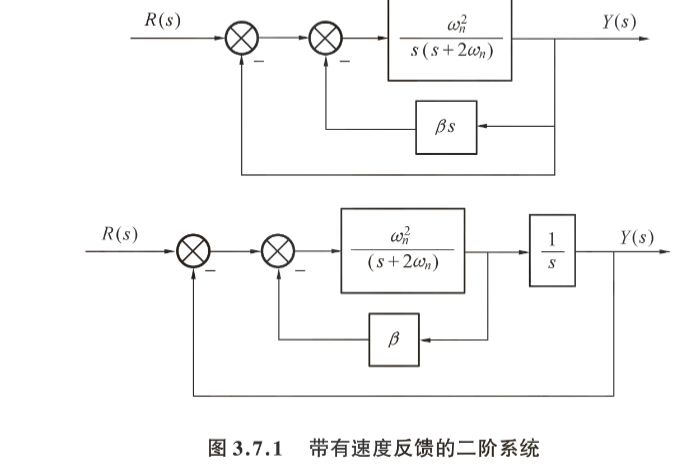
\includegraphics[width = .4\textwidth]{note/time-domain analysis/figure/7.png}
\end{center}

引入速度反馈后，系统的闭环传递函数为：
\begin{equation*}
    \varPhi(s) = \frac{Y(s)}{R(s)} = \frac{\omega_n^2}{s^2 + (2\zeta \omega_n + \omega_n^2 \beta)+\omega_n^2} = \frac{\omega_n^2}{s^2 + 2\overline{\zeta} \omega_n s + \omega_n^2}
\end{equation*}

显然，在引入速度反馈后，系统的阻尼比$\overline{\zeta}$要比原阻尼比$\zeta$要大
\begin{example}
    二阶系统的方框图如图所示，要求闭环系统的超调量$\sigma_p = 16.3\%$，峰值时间$t_p = 1$s，求放大器的放大倍数$K_0$和速度反馈系数$\tau$
    \begin{center}
        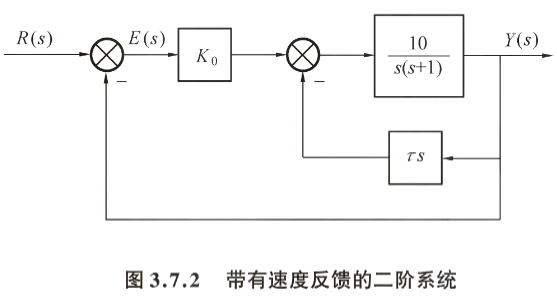
\includegraphics[width = .3\textwidth]{note/time-domain analysis/figure/8.png}
    \end{center}
    \textbf{解}：带有速度反馈系统的开环传递函数$G(s)$和闭环传递函数分别为：
    \begin{equation*}
        \begin{split}
            G(s) &= \frac{10K_0}{s^2 + (1+10\tau)s} \\
            \varPhi(s) &=\frac{10K_0}{s^2+(1+10\tau)s + 10K_0}
        \end{split}
    \end{equation*}

    由系统的闭环传递函数可以得出：
    \begin{equation*}
        \begin{split}
            \omega_n^2 &= 10K_0 \\
            2\zeta \omega_n &= 1+10\tau
        \end{split}
    \end{equation*}
    由已知可得：
    \begin{equation*}
        \begin{split}
            \sigma_p &= e^{-\zeta \pi /\sqrt{1-\zeta^2}}  = 0.163\\
            t_p/\mathrm{s} &= \frac{\pi}{\omega_n \sqrt{1-\zeta^2}} =1
        \end{split}
    \end{equation*}

    解得：$K_0 = 1.32,\tau = 0.263$
\end{example}

\subsection{PD控制}
如图所示为PD控制系统示意图：
\begin{center}
    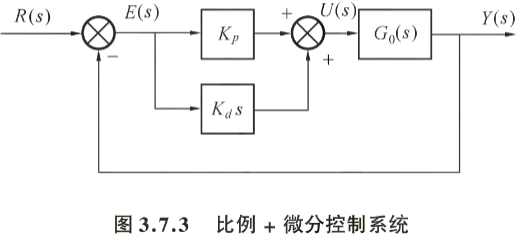
\includegraphics[width = .3\textwidth]{note/time-domain analysis/figure/9.png}
\end{center}

由图可知PD控制器的传递函数为：
\begin{equation*}
    G_c(s) = \frac{U(s)}{E(s)} = K_p + K_d s = K_p(1+\frac{K_d}{K_p}s) = K_p(1+\tau s)
\end{equation*}

下面以欠阻尼二阶系统为例讨论PD控制对改善系统动态过程的作用：
\begin{example}
    在图3.7.3中，设$G_0 (s) = \dfrac{K_0}{s(Ts+1)} $ 则：\\
    在没有PD校正的情况下，系统的闭环传递函数为：
    \begin{equation*}
        \varPhi(s) = \frac{K_0}{Ts^2+s+K_0}
    \end{equation*}

    此时$\omega_n = \sqrt{K_0/T},\zeta = 0.5 \sqrt{K_0 T}$\\

    采用PD校正后的传递函数为：
    \begin{equation*}
        \overline{\varPhi}(s) = \frac{K_0 K_p (\tau s + 1)}{Ts^2 + (K_0 K_p \tau+1)s + K_0 K_p}
    \end{equation*}

    此时相应的参数变化为：$\overline{\omega_n} = \sqrt{\dfrac{K_0 K_p}{T}} , \overline{\zeta} = \frac{K_0 K_p \tau +1}{2 \sqrt{T K_0 K_p}}$\\

    其中$\tau = \dfrac{K_d}{K_p}$

    对比前后参数的变化，可以看到：只要适当选取$K_p , K_d$的值，就可以增大系统无阻尼振荡频率和阻尼比，使系统的快速性和平稳性都得到改善。
\end{example}



\chapterimage{11.jpg}
\chapter{频域分析}

\section{频率特性}

\begin{definition}{频率特性}
    \label{frequency-characteristics}
    我们称$G(j\omega)$为系统（或元件）的频率特性，又称频率响应，可以由系统的传递函数求得：
    \begin{equation*}
        G(j\omega) = G(s)|_{s=j\omega} = \left\lvert G(j\omega) \right\rvert e^{j\phi(\omega)} 
    \end{equation*}

    其中$\phi(\omega) = \angle G(j\omega)$

    频率特性具有以下性质：
    \begin{enumerate}
        \item 频率特性是描述线性定常系统的一种数学模型，只有线性定常系统才有频率特性
        \item 频率特性$G(j\omega)$是一个复变量，它的幅值$\left\lvert G(j\omega) \right\rvert $ 和相角$\phi(\omega)$ 都是频率$\omega$的函数
        \item 系统在频率为$\omega$的正弦输入信号作用下，频率特性反映了输出信号稳态分量和输入信号的关系
        \item 在频率特性中，所用的频率均为角频率$\omega$
        \item 在频率特性中，一般讨论的频率范围是$\omega \in (0,+\infty)$
        \item 频率特性的另一个定义是：频率特性是输出信号Fourier变换式与输入信号Fourier变换式之比
        \item 频率特性是系统脉冲响应的Fourier变换式
    \end{enumerate}
\end{definition}

\subsection{频率特性的几种表示形式}

频率特性$G(j\omega)$是一个复变函数，它是$\omega$的函数。对于连续变化的$\omega$，$G(j\omega)$是复数平面上的一条轨迹

频率特性有以下几种表示形式
\subsubsection{Nyquist图}
将频率特性$G(j\omega)$写成模和幅角的形式，让$\omega$从0变化至$+\infty$，将$G(j\omega)$的轨迹画在复数平面中，即是Nyquist图

典型环节的Nyquist图如下所示：
\begin{center}
    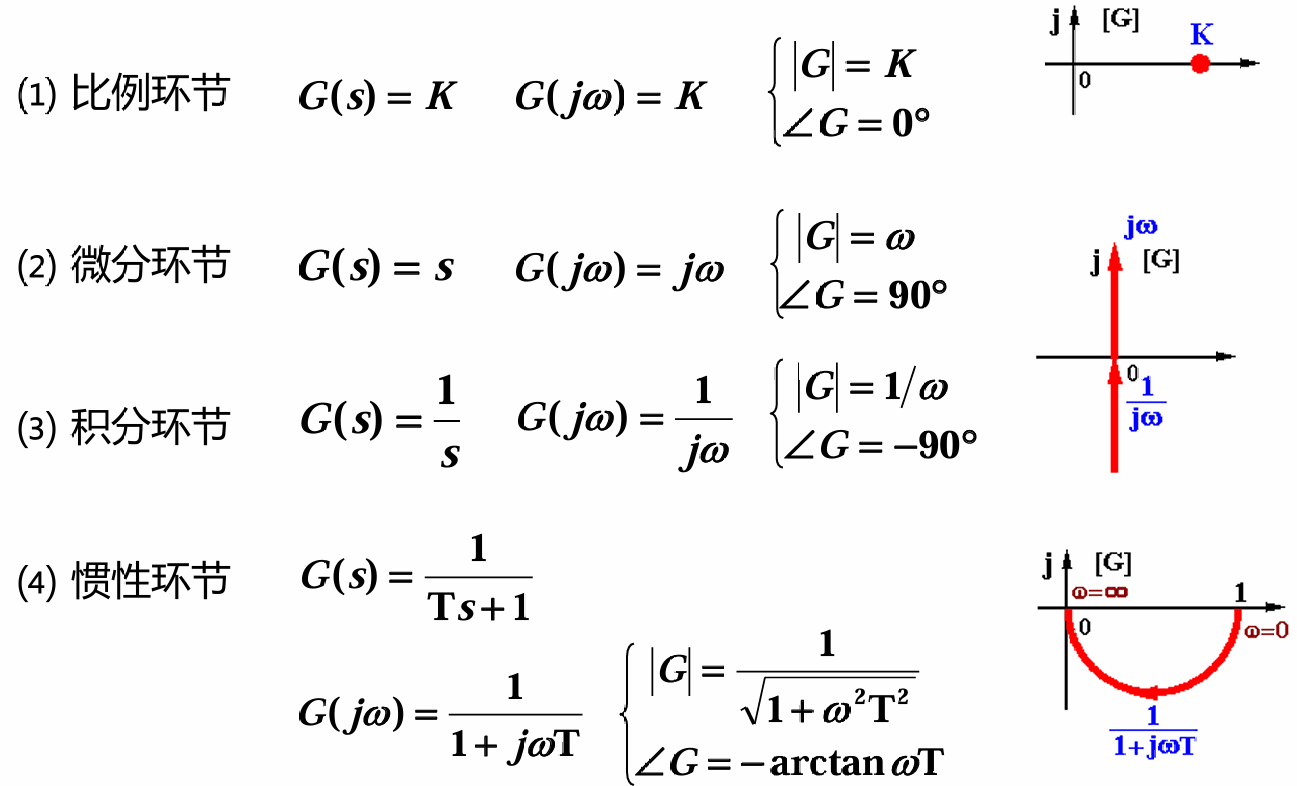
\includegraphics[width=.5\textwidth]{note/frequency-domain analysis/figure/1.png}\\
    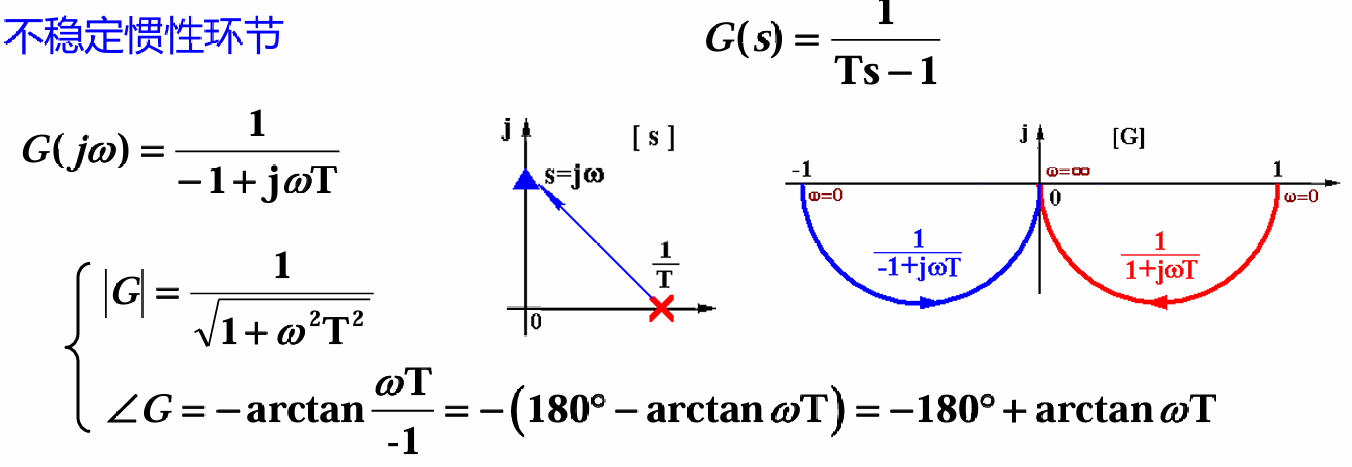
\includegraphics[width=.5\textwidth]{note/frequency-domain analysis/figure/2.png}\\
    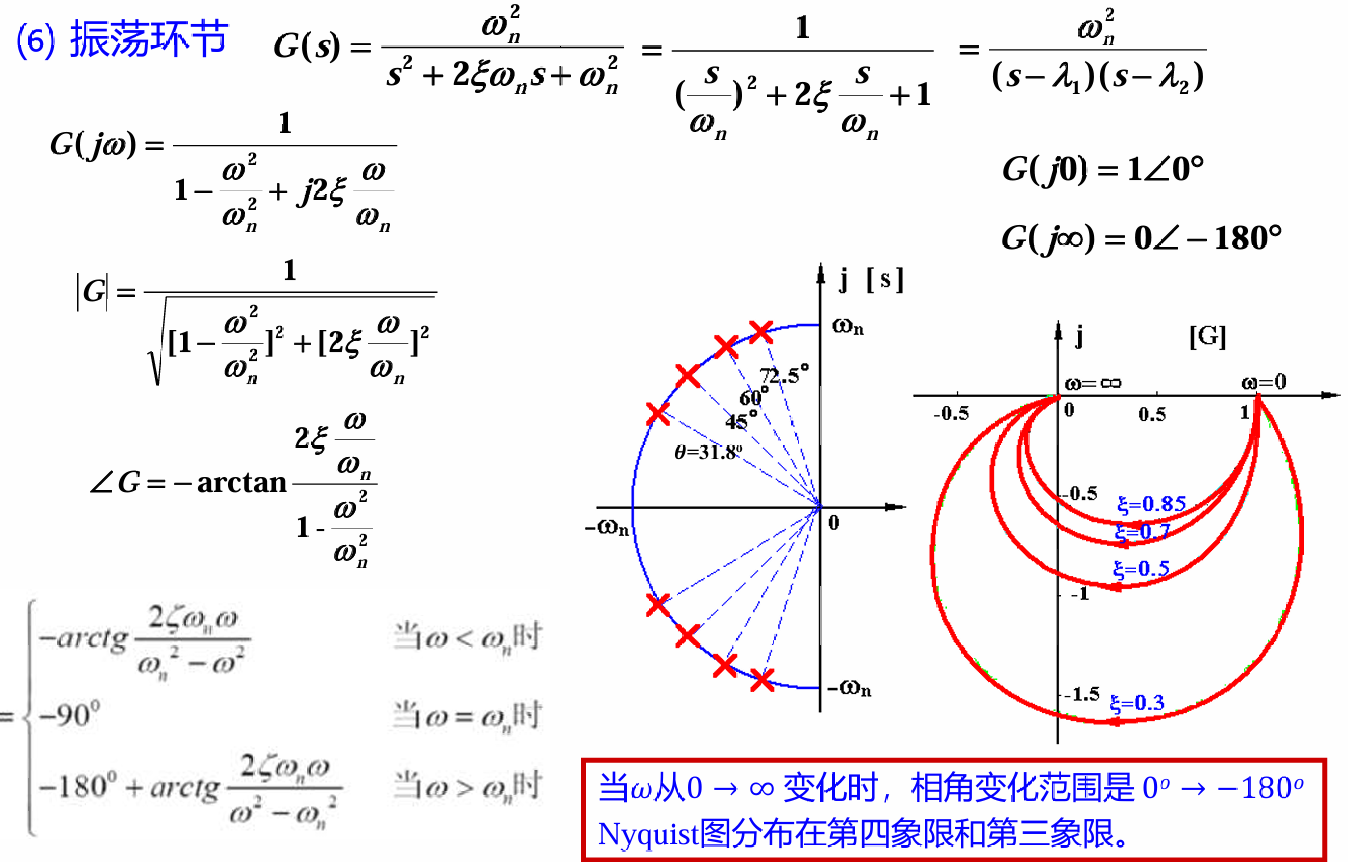
\includegraphics[width=.5\textwidth]{note/frequency-domain analysis/figure/3.png}\\
    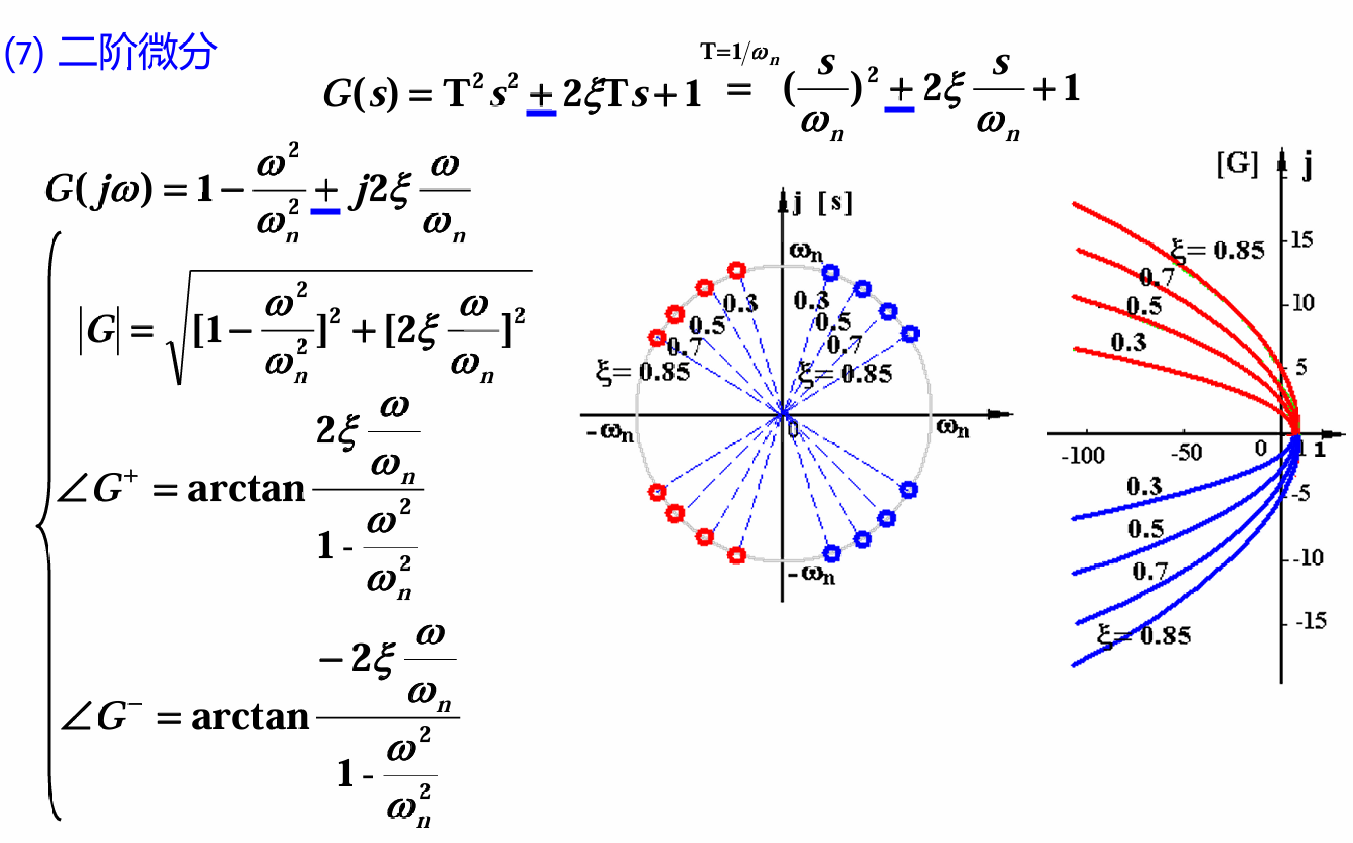
\includegraphics[width=.5\textwidth]{note/frequency-domain analysis/figure/4.png}\\
    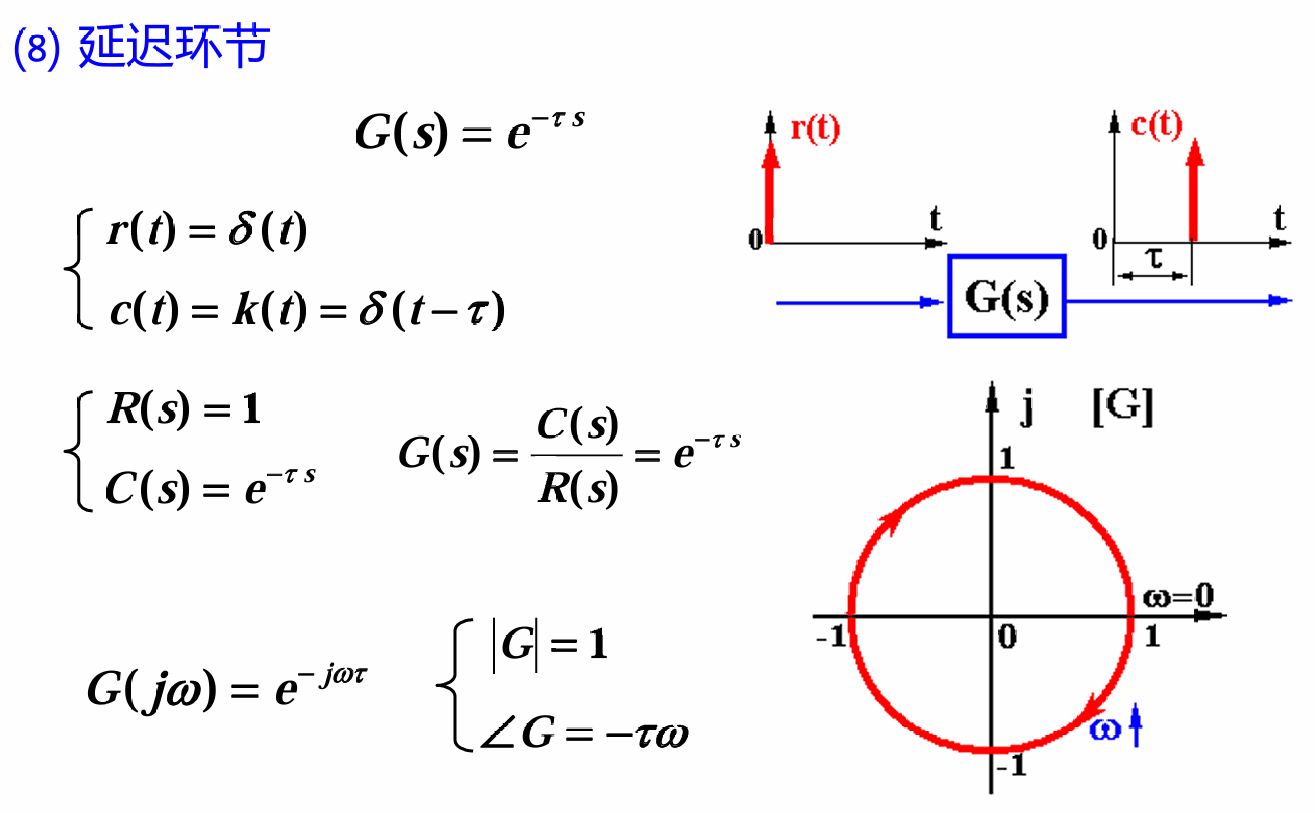
\includegraphics[width=.5\textwidth]{note/frequency-domain analysis/figure/5.png}\\
\end{center}

一般频率特性的Nyquist图绘制法如下：
\begin{enumerate}
    \item 当$\omega = 0$时，比例环节、惯性环节、振荡环节、一阶和二阶微分环节的幅角均为0°，只有积分环节当$\omega = 0^+$时幅角为-90°，所以当系统的开环传递函数中含有$v$个串联积分环节时，开环频率特性的Nyquist图在$\omega = 0^+$的起始处幅角为$v\cdot(-90\text{°})$
    \item 当$\omega = 0$时，比例环节的幅值为$K$，积分环节在$\omega = 0^+$时的幅值为$\infty$，其余各环节的幅值均为1，所以，开环幅频特性的幅值为：无积分环节$\omega = 0$时的幅值为$K$；有积分环节$\omega = 0^+$时幅值为$\infty$
    \item 当$\omega \to +\infty$时，开环频率特性Nyquist图中曲线的切线方向是$(n-m)\cdot(-90\text{°})$，其中m是分子的阶次，n是分母的阶次
    \item 当$\omega\to +\infty$时，开环频率特性Nyquist图沿$(n-m)\cdot(-90\text{°})$的方向趋向原点
\end{enumerate}
注意：
\begin{enumerate}
    \item 一个特殊点：谐振点：频率特性的幅值达到峰值的点（一般只有振荡环节存在），计算式如下：
    \begin{equation*}
        \omega_r = \omega_n\sqrt{1-2\zeta^2}
    \end{equation*}
    此时的峰值为：
    \begin{equation*}
        M_r = \left\lvert G(j\omega_r) \right\rvert =\frac{1}{2\zeta\sqrt{1-\zeta^2}}
    \end{equation*}
    \item 对于度数所对应的方向为：0°朝左，90°朝上，180°朝右，270°朝下
    \item 实际绘图时先把系统的频率特性（幅频和相频）写出来，观察式子中是否有间断点再绘图
\end{enumerate}



\subsubsection{Bode图}

频率特性$G(j\omega)$中的幅频特性和相频特性都是$\omega$的函数，Bode图是按照以下规律绘制的：
\begin{enumerate}
    \item 把幅频特性和相频特性分开画，横坐标为角频率$\omega$，纵坐标分别是频率特性的幅值和相角，画成两个曲线
    \item 在画频率特性时，角频率$\omega$的变化范围很大，几乎为$0\to +\infty$，所以将横坐标以10为底$\omega$的对数为长度划分，定义横坐标上每10倍频程之间的距离为一个单位长度，称作十倍频程（dec）
    \item 在Bode图的幅频特性中，纵坐标使用$L(\omega)$：
    \begin{equation*}
        L(\omega) = 20 \lg \left\lvert G(j\omega) \right\rvert 
    \end{equation*}

    此时即可将相乘转化为相加
    \item 在Bode图中，相频特性曲线的纵坐标时相频特性的角度本身$\angle G(j\omega)$，一般用°为单位，也可用弧度为单位
\end{enumerate}

典型环节的Bode图绘制如下所示：
\begin{center}
    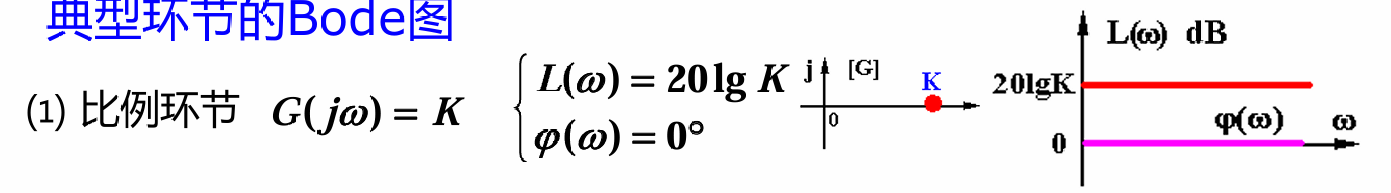
\includegraphics[width = .5\textwidth]{note/frequency-domain analysis/figure/6.png}\\
    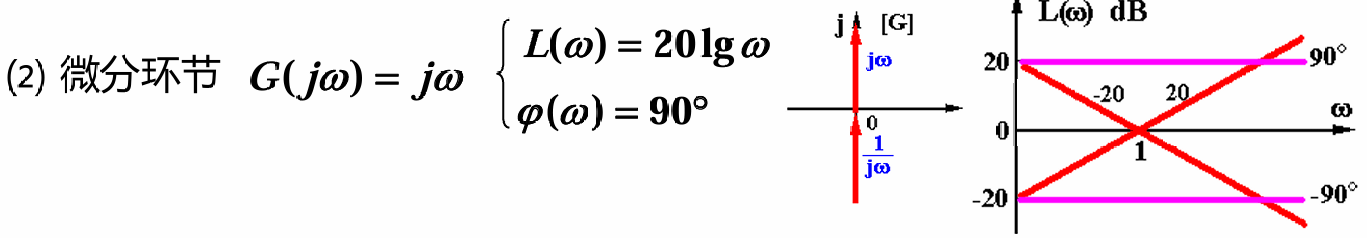
\includegraphics[width = .5\textwidth]{note/frequency-domain analysis/figure/7.png}\\
    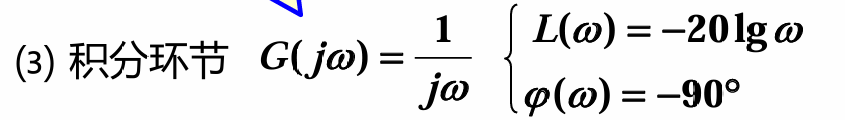
\includegraphics[width = .5\textwidth]{note/frequency-domain analysis/figure/8.png}\\
    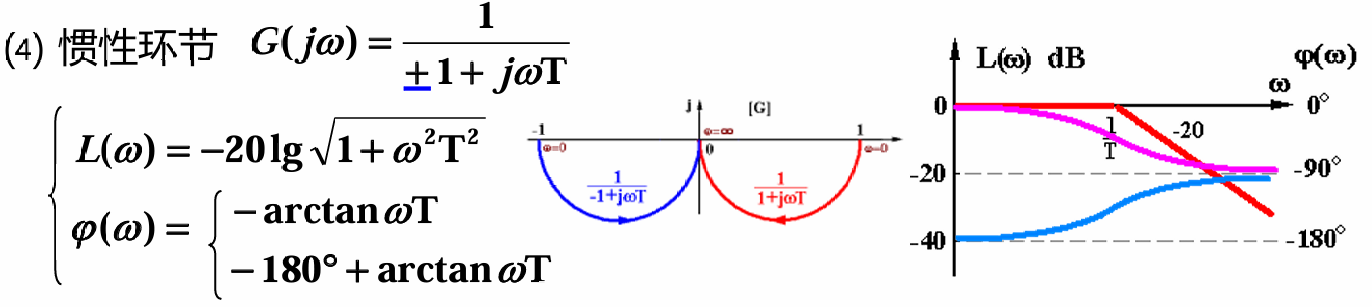
\includegraphics[width = .5\textwidth]{note/frequency-domain analysis/figure/9.png}\\
    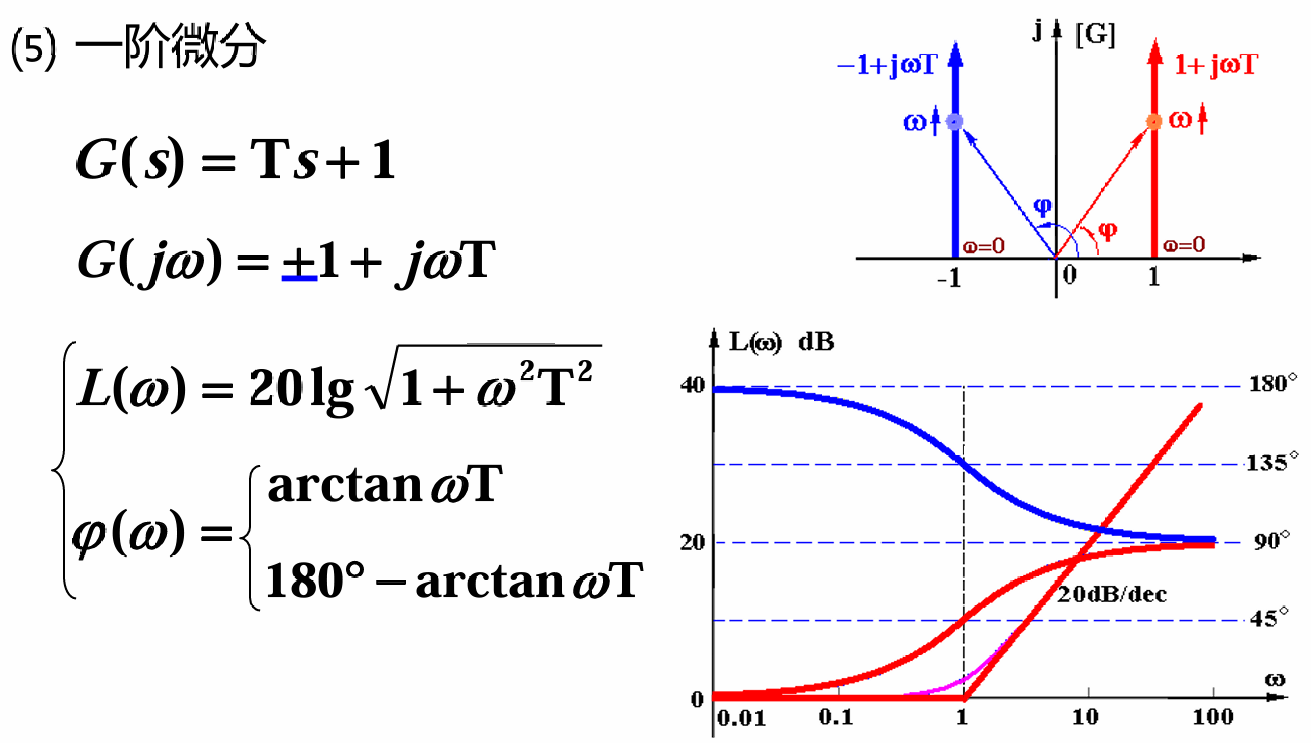
\includegraphics[width = .5\textwidth]{note/frequency-domain analysis/figure/10.png}\\
    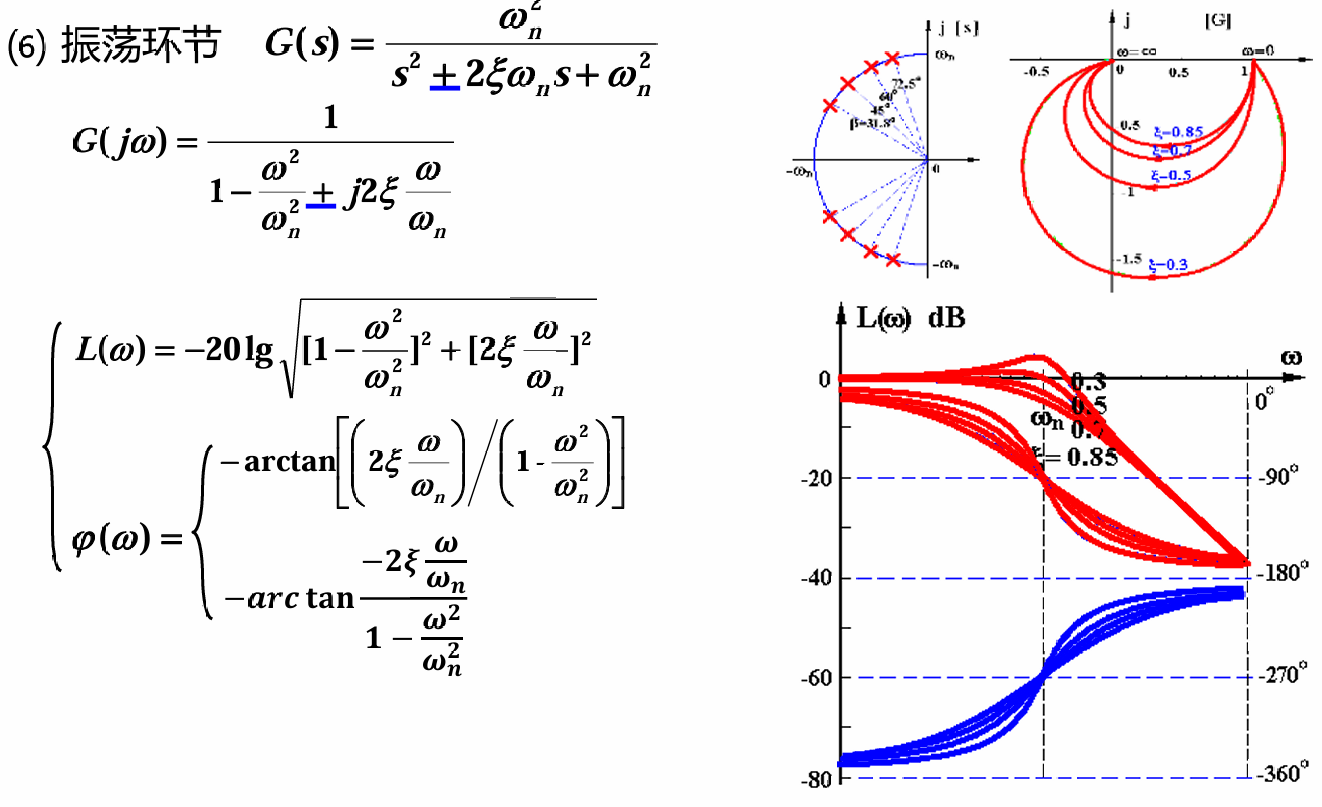
\includegraphics[width = .5\textwidth]{note/frequency-domain analysis/figure/11.png}\\
    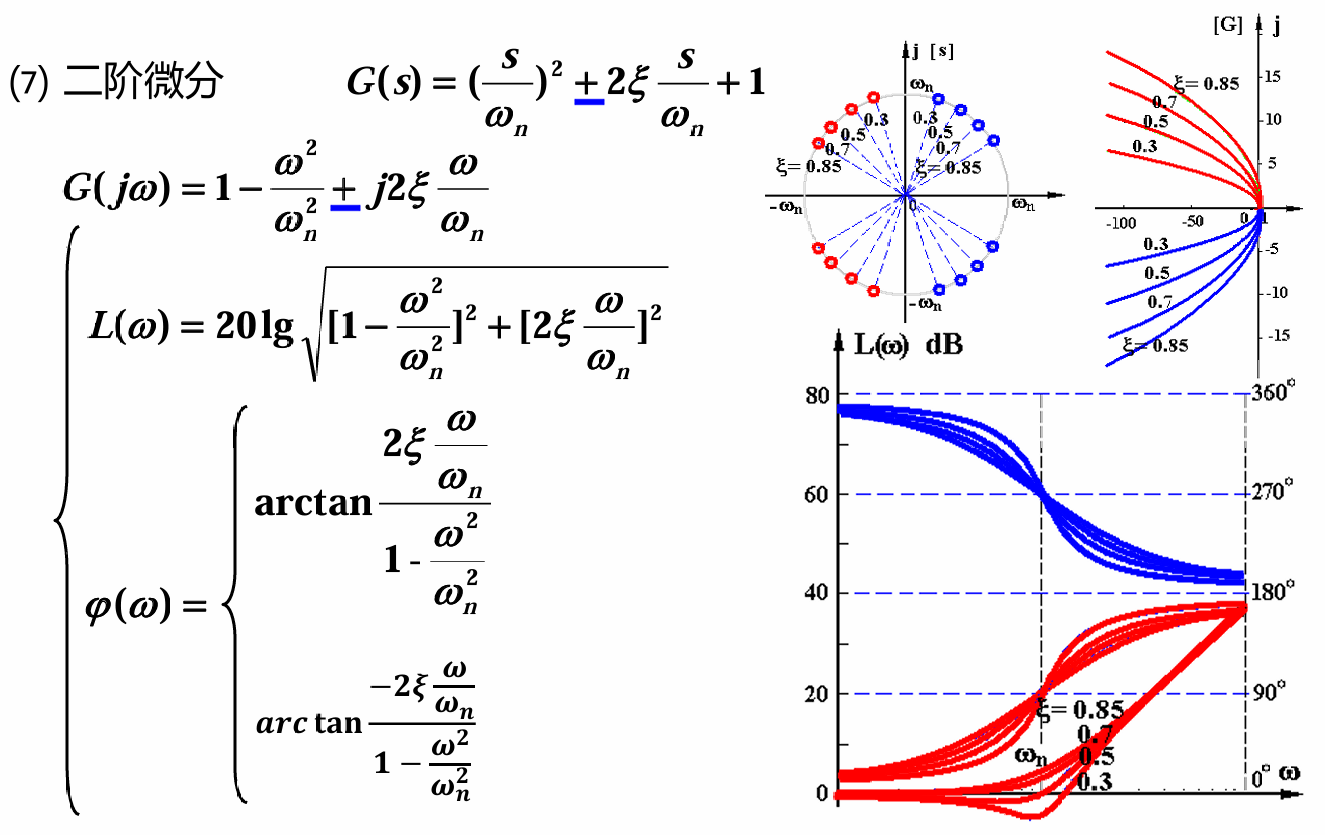
\includegraphics[width = .5\textwidth]{note/frequency-domain analysis/figure/12.png}\\
    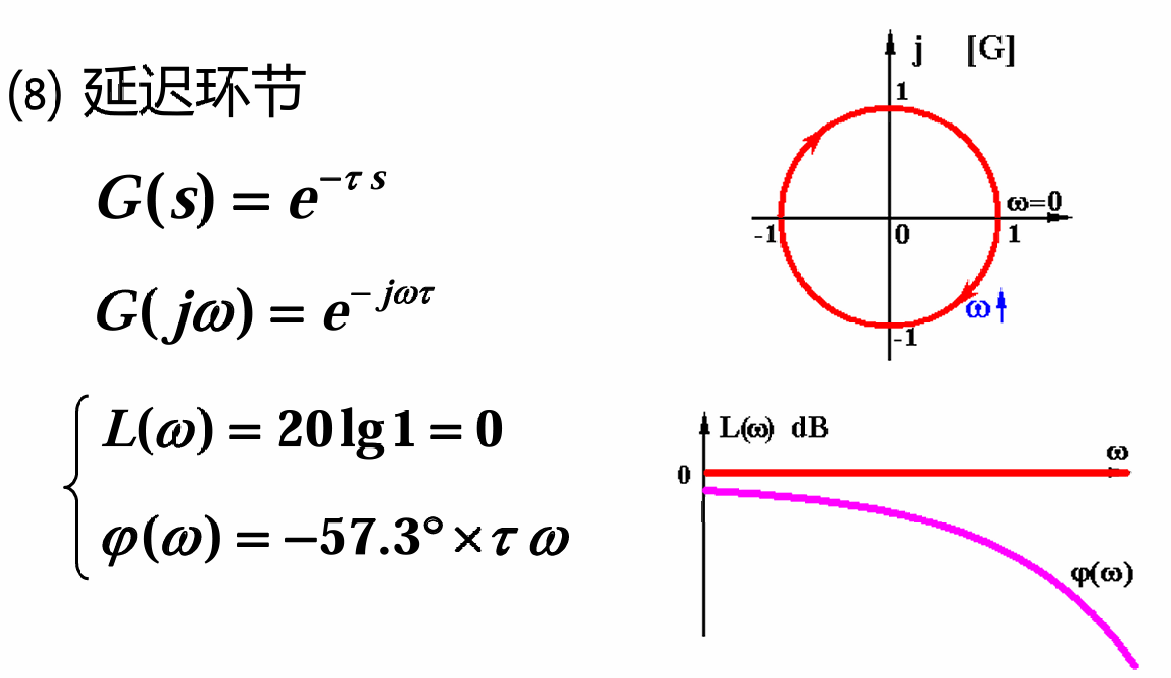
\includegraphics[width = .5\textwidth]{note/frequency-domain analysis/figure/13.png}
\end{center}

同样的，注意一个特殊点：剪切频率：Bode图中幅值特性第一次等于零的点，记为：$\omega_c$

\textbf{一般频率特性的Bode图的绘制}：

对数幅频特性与对数相频特性分别是各个串联环节的对数幅频特性之和与对数相频之和，所以只需做出各个环节的Bode图后将对应的幅频特性曲线与各个相频特性曲线相加即可，具体如下：
\begin{enumerate}
    \item 将$G(s)$化为频率特性标准型
    \item 按照顺序列出各个串联环节的转折频率（简化Bode图中斜率变化的点）
    \item 确定基准线（最小转折频率之左的特性及其延长线），此线过（1，$20\lg K$）
    \item 叠加作图（一阶$\pm 20$，二阶$\pm 40$）
    \item 在以下情况下修正简化Bode图：
    \begin{enumerate}
        \item 两惯性环节转折频率很接近时
        \item 振荡环节或二阶微分环节，此处有两种修正方式：
        \begin{itemize}
            \item 转折频率处修正，此时幅值差值（实际值-拟合值or虚线值-实线值）=$20\lg(\dfrac{1}{2\zeta})$（振荡环节）or = $20\lg(2\zeta)$（二阶微分环节）
            \item 谐振频率处修正，此时峰值$M_r = \dfrac{1}{2\zeta\sqrt{1-\zeta^2}}$，谐振频率$\omega_r = \omega_n\sqrt{1-2\zeta^2}$，bode图中为实际值-拟合值的绝对值为$20\lg M_r$
        \end{itemize}
    \end{enumerate}
    \item 检查Bode图是否正确：
    \begin{enumerate}
        \item 幅值特性曲线最右端斜率=-20(n-m)dB/dec
        \item 转折点数=惯性环节数+一阶微分数+振荡环节数+二阶微分数
        \item 相频特性在无穷处大小$\phi(\omega)\to -90\text{°}(n-m)$
    \end{enumerate}
\end{enumerate}

\chapterimage{12.jpg}
\chapter{线性离散系统}

\section{A/D转换}

\subsection{A/D转换}

A/D转换器将模拟信号变成数字信号。A/D转换的过程可以看作是采样、量化和编码过程

采样的过程如下图所示，假设采样开关每隔一定时间$T$闭合一次，则称$T$为采样周期，则采样频率为
\begin{center}
    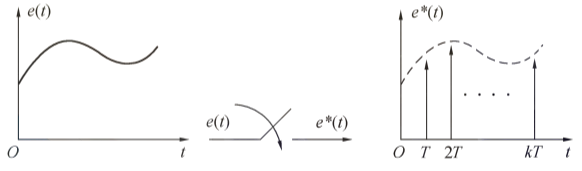
\includegraphics[width = .6\textwidth]{note/linear discrete system/figure/1.png}
\end{center}

\begin{equation*}
    f_s = \frac{1}{T}
\end{equation*}

而采样角频率为
\begin{equation*}
    \omega_s = \frac{2\pi}{T} = 2\pi f_s
\end{equation*}

采样过程可以看作是一个脉冲调制过程。设理想的单位脉冲序列为：
\begin{equation*}
    \delta_T (t) = \sum_{k=0}^\infty \delta(t-kT)
\end{equation*}

由此可以得到模拟信号的采样信号为：
\begin{equation*}
    e^* (t) = e(t) \delta_T(t) = \sum_{k=0}^\infty e(KT) \delta(t-KT)
\end{equation*}

量化就是采用有限字长的一组二进制数去逼近离散模拟信号的幅值。在计算机中，任何数值都可以表示成二进制数字量最低位的整数倍。数字量最低为所代表的数值称为量化单位通常用$q$来表示

编码就是将量化后的数值变成按某种规则编码的二进制数码。常用的编码形式有：原码，补码，偏移码、BCD码等。

\subsection{离散信号的频谱}

对于一个频谱有限连续时间信号$x(t)$，其Fourier变换为：
\begin{equation*}
    X(j\omega) = \int^\infty_{-\infty} x(t)e^{-j\omega t} dt
\end{equation*}

同样的，对于一个理想采样信号$x^* (t) = x(t) \delta_T(t) = \sum\limits_{k=0}^\infty x(KT) \delta(t-KT)$，我们可以写出他的Fourier变换：
\begin{equation*}
    X_s(\omega) = \frac{1}{2\pi} X(\omega)*(\omega_s \sum\limits_{n=-\infty}^{+\infty} \delta(\omega-n\omega_s)) = \frac{1}{T_s}\sum\limits_{n=-\infty}^{+\infty}X(\omega-n\omega_s)
\end{equation*}

考虑需要不失真地恢复原来的连续信号，理想采样角频率需要满足以下定理：

\begin{theorem}[Shannon定理]
    对于频谱有限信号$x(t)$，如果其最高频率分量为$\omega_m$，为了保留原信号的全部信息，或能无失真地恢复原信号，在通过采样得到离散信号时，其采样频率应满足$\omega_s\geq 2\omega_m$。通常把最低允许的采样频率$\omega_s = 2\omega_m$称为Nyquist频率，最大允许采样间隔$T_s = \dfrac{\pi}{\omega_m}$称为Nyquist间隔
\end{theorem}

在工程实际中，采样角频率往往取的比Nyquist频率要大得多

\subsection{采样周期的选取}

在Shannon定理中，采样周期需要越小越好，但是在工程实际中，采样周期取得过短，将会增加不必要的计算负担。反之，采样周期取得过长，又会给控制过程带来较大的误差，降低系统的动态性能

所以，根据工程实践的经验，伺服系统的采样频率可选为：
\begin{equation*}
    \omega_s \approx 10\omega_c
\end{equation*}

其中$\omega_c$为开环系统的幅值穿越频率


\section{D/A转换}
D/A转换器将数字信号转换为模拟信号。D/A转换的过程可以看成是解码和保持的过程

解码就是根据D/A转换器所采用的编码规则，将数字信号折算成对应的电压或电流值。这个电压或电流值仅仅是对应各采样时刻的，而相邻两采样时刻之间的值还没有确定。

保持就是解决各相邻采样时刻之间的插值问题，将离散时间信号变成连续时间信号。实现保持功能的器件称为保持器。保持器有各种类型，D/A转换器中一般使用零阶保持其，其传递函数通常记为$H_0(s)$。零阶保持器是一种具有常值外推功能的保持器，它将采样时刻的电压或电流值不增不减地保持到下一个采样时刻到来之前。

\section{Z变换与Z反变换}

\subsection{Z变换}

考虑一个对连续信号进行理想采样的离散信号：
\begin{equation*}
    x^* (t) = x(t) \delta_T(t) = \sum\limits_{k=0}^\infty x(KT) \delta(t-KT)
\end{equation*}

其Laplace变换为：
\begin{equation*}
    X^*(s) = \sum_{k=0}^\infty x(kT)e^{-kTs}
\end{equation*}

记复变量$z = e^{-Ts}$，则上式可以写为：
\begin{equation*}
    X(z) = \sum_{k=0}^\infty x(kT)z^{-k}
\end{equation*}

\begin{definition}
    称式子
    \begin{equation*}
    X(z) = \sum_{k=0}^\infty x(k)z^{-k}
    \end{equation*}
    为离散信号$x(k)$的Z变换，记为：$X(z) = Z[x(t)]$

    \textbf{注}：
    \begin{enumerate}
        \item     在本笔记中，记连续信号$x(t)$理想采样各个值$x(kT)$为$x(k)$，与信号分析与处理类似
        \item 默认连续信号存在Z变换，且其Z变换与其理想采样信号的Z变换相同
    \end{enumerate}


    
\end{definition}

\subsection{求Z变换的常用方法}

\subsubsection{级数求和法}

由Z变换的定义可以得到：
\begin{equation*}
    X(z) = x(0) + x(1) z^{-1} + x(2) z^{-2} + \cdots + x(k) z^{-k} +\cdots
\end{equation*}

这是$X(z)$的laurent级数表达式，故只要知道$x(k)$的闭式表达，即可求出其Z变换

\subsubsection{部分分式法}


\partsimage{cov18.pdf}
\part{现代控制理论}

\chapterimage{8.jpg}
\chapter{状态空间模型}

\section{线性系统的状态空间描述}

\subsection{线性系统的状态空间描述}

\begin{definition}[状态与状态空间]
    完全地表征系统时间域行为的最小个数的内部变量组称为系统的状态。组成这个变量组的变量$x_1(t),x_2(t),\cdots,x_n(t)$称为系统的状态变量，其中，$t \geq t_0$，$t_0$为系统的初始时刻。由状态变量构成的列向量
    \begin{equation*}
        \bm{x}(t) = \left[
            \begin{array}{c}
                x_1(t) \\ x_2(t) \\ \vdots \\ x_n(t)\\
            \end{array}
        \right] \quad t \geq t_0
    \end{equation*}

    称为系统的状态向量，简称为状态。状态向量的取值的向量空间称为状态空间。
\end{definition}

对于以上的定义，有如下几点需要注意：
\begin{enumerate}
    \item “完全表征系统时间域的行为”是指给定状态变量的初值，以及系统的输入信号，则系统在$t \geq t_0$时间域上的运动行为完全确定
    \item 状态变量组的“最小数目”的含义为状态变量$x_1(t),x_2(t),\cdots,x_n(t)$是能够完全表征系统运动特性的变量的最小个数，减少变量个数将不能完全表征系统
    \item 考虑系统内部的各个变量，则$x_1(t),x_2(t),\cdots,x_n(t)$构成系统变量中线性无关的一个极大无关组。具有$n$维状态变量的全体就构成了实数域上的$n$维空间
\end{enumerate}

\begin{corollary}
    一个动态系统任意选取的两个状态变量组之间为线性非奇异变换的关系（基变换关系）
\end{corollary}

\begin{definition}[状态方程与输出方程]
    输入引起状态变化的过程写成状态变量的一阶微分方程组的形式，称为系统的状态方程，即：
    \begin{equation*}
        \begin{split}
            \dot{x_1} &= f_1(x_1,x_2,\cdots,x_n;u_1,u_2,\cdots,u_r;t) \\
            \vdots & \\
            \dot{x_n} &= f_n(x_1,x_2,\cdots,x_n;u_1,u_2,\cdots,u_r;t) \\
        \end{split}
    \end{equation*}

    其中，$t\geq t_0$。在引入向量表示的基础上，可以将状态方程表示为向量方程的形式
    \begin{equation*}
        \dot{\bm{x}} = \bm{f}(\bm{x},\bm{u},t) \quad t \geq t_0
    \end{equation*}

    其中
    \begin{equation*}
        \bm{x}(t) = \left[
            \begin{array}{c}
                x_1(t) \\ \vdots \\ x_n(t) 
            \end{array}
        \right]
        \quad
        \bm{u} = \left[
            \begin{array}{c}
                u_1 \\ \vdots \\ u_r
            \end{array}
        \right]
        \quad 
        \bm{f}(\bm{x},\bm{u},t) = \left[
            \begin{array}{c}
                f_1(\bm{x},\bm{u},t) \\ \vdots \\ f_n(\bm{x},\bm{u},t)
            \end{array}
        \right]
    \end{equation*}

    类似，状态和输入决定输出变化，可以用如下的输出方程表示，即：
        \begin{equation*}
        \begin{split}
            \dot{y_1} &= g_1(x_1,x_2,\cdots,x_n;u_1,u_2,\cdots,u_r;t) \\
            \vdots & \\
            \dot{y_m} &= g_m(x_1,x_2,\cdots,x_n;u_1,u_2,\cdots,u_r;t) \\
        \end{split}
    \end{equation*}

    或者表示成向量方程的形式
        \begin{equation*}
        \bm{y} = \bm{g}(\bm{x},\bm{u},t) 
    \end{equation*}

    其中
    \begin{equation*}
        \bm{y}(t) = \left[
            \begin{array}{c}
                y_1(t) \\ \vdots \\ y_m(t) 
            \end{array}
        \right]
        \quad
        \bm{u} = \left[
            \begin{array}{c}
                u_1 \\ \vdots \\ u_r
            \end{array}
        \right]
        \quad 
        \bm{g}(\bm{x},\bm{u},t) = \left[
            \begin{array}{c}
                g_1(\bm{x},\bm{u},t) \\ \vdots \\ g_m(\bm{x},\bm{u},t)
            \end{array}
        \right]
    \end{equation*}
\end{definition}

系统的状态空间描述由状态方程和输出方程所组成，联合写出，则为：
\begin{equation*}
    \begin{aligned}
        \dot{\bm{x}} &= \bm{f}(\bm{x},\bm{u},t) \quad t \geq t_0 \\ 
        \dot{\bm{y}} &= \bm{g}(\bm{x},\bm{u},t)   \\
    \end{aligned}
\end{equation*}

如果考察线性系统的连续动态过程，可以将上述两个方程写成如下形式：
\begin{equation*}
    \begin{aligned}
        \dot{\bm{x}} &= \bm{A}(t) \bm{x} + \bm{B}(t) \bm{u} \quad t \geq t_0 \\
        \bm{y} &= \bm{C}(t) \bm{x} + \bm{D}(t) \bm{u}
    \end{aligned}
\end{equation*}

如果考察线性定常系统，则上述两个方程还能进行简化：
\begin{equation*}
    \begin{aligned}
        \dot{\bm{x}} &= \bm{A} \bm{x} + \bm{B} \bm{u} \quad t \geq t_0 \\
        \bm{y} &= \bm{C} \bm{x} + \bm{D} \bm{u}
    \end{aligned}
\end{equation*}

\subsection{状态空间表达式的建立}
系统的状态空间描述一般可以从三个途径求得：
\begin{enumerate}
    \item 由系统方框图建立，即根据系统各个环节的实际连结，写出相应的状态空间表达式
    \item 从系统的物理或者化学机理出发推导
    \item 由描述系统运动过程的高阶微分方程予以演化得到
\end{enumerate}

\subsubsection{从系统方框图建立状态空间表达式}
\begin{example}
    系统方框图如图所示，输入为$u$，输出为$y$，求其状态空间表达式
    \begin{center}
        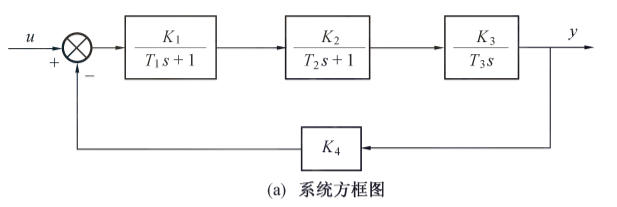
\includegraphics[width = 0.6\textwidth]{note/state space/figure/1.png}
    \end{center}

    \textbf{解}：各环节的模拟结构图下图所示：
    \begin{center}
        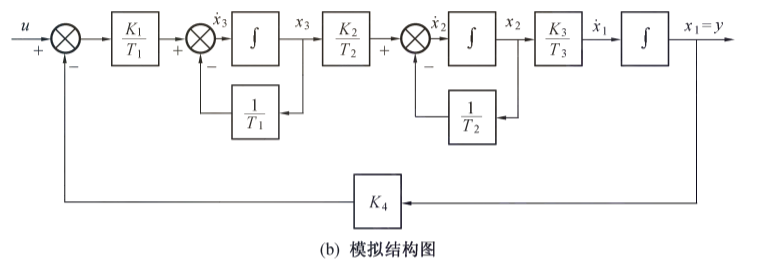
\includegraphics[width = 0.6\textwidth]{note/state space/figure/2.png}
    \end{center}

    由模拟结构图可以得到系统的状态方程为：
    \begin{equation*}
        \begin{aligned}
            \dot{x_1} &= \frac{K_3}{T_3} x_2 \\
            \dot{x_2} &= -\frac{1}{T_2} x_2 + \frac{K_2}{T_2} x_3 \\
            \dot{x_3} &= -\frac{1}{T_1}x_3 - \frac{K_1K_4}{T_1} x_1 + \frac{K_1}{T_1} u\\
        \end{aligned}
    \end{equation*}

    $y = x_1$ 为系统输出方程，写成向量和矩阵的形式，系统的状态空间表达式为：
    \begin{equation*}
        \begin{aligned}
            \dot{\bm{x}} &= \left[
                \begin{array}{ccc}
                    0 & \frac{K_3}{T_3} & 0 \\
                    0 & -\frac{1}{T_2} & \frac{K_2}{T_2} \\
                    -\frac{K_1K_4}{T_1} & 0 & -\frac{1}{T_1} \\
                \end{array}
            \right]
            \bm{x} + \left[
                \begin{array}{c}
                    0 \\ 0 \\ \frac{K_1}{T_1}
                \end{array}
            \right] u \\
            y &= \left[
                \begin{array}{ccc}
                    1 & 0 & 0\\
                \end{array}
            \right] \bm{x}
        \end{aligned}
    \end{equation*}
\end{example}

\subsubsection{从系统的机理出发建立状态空间表达式}
\begin{example}
    电网络如下图所示：输入量为电流源，输出变量取为电阻的输出电压，求此网络的状态空间表达式
    \begin{center}
        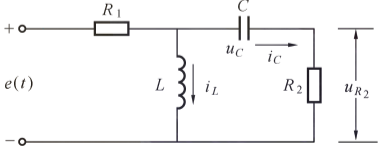
\includegraphics[width = .6\textwidth]{note/state space/figure/3.png}
    \end{center}

    \begin{enumerate}
        \item 确定状态变量，一般选取独立储能元件的线性无关变量作为状态变量。这里选取电容电压$u_C$和电感电流$i_L$作为电路的状态变量
        \item 列出电路方程：
        \begin{equation*}
            \begin{cases}
                R_1(i_C + i_L) + L \frac{di_L}{dt} = e(t) \\
                u_C + R_2 i_C = L \frac{di_L}{dt} \\
                i_C = C \frac{du_C}{dt}
            \end{cases}
        \end{equation*}
        \item 列写状态方程组和输出方程组。状态方程组为：
        \begin{equation*}
            \begin{cases}
                \frac{du_C}{dt} = - \frac{1}{(R_1+R_2)C}[u_C+R_1 i_L - e(t)]\\
                \frac{d i_L}{dt} = \frac{1}{L(R_1+R_2)}[R_1 u_C - R_1 R_2 i_L + R_2 e(t)]
            \end{cases}
        \end{equation*}

        输出方程为：
        \begin{equation*}
            u_{R_2} = R_2 i_C = R_2 C \frac{du_C}{dt} = -\frac{R_2}{R_1 + R_2}[u_C + R_1 i_L - e(t)]
        \end{equation*}

        \item 写成向量形式：
        \begin{equation*}
            \begin{split}
                &\left[
                    \begin{array}{c}
                        \frac{du_C}{dt} \\ \frac{di_L}{dt}
                    \end{array}
                \right] = 
                \left[
                    \begin{array}{cc}
                        -\frac{1}{(R_1 + R_2)C} & -\frac{R_1}{(R_1+R_2)C} \\
                        \frac{R_1}{L(R_1+R_2)} & -\frac{R_1 R_2}{L(R_1+R_2)}
                    \end{array}
                \right]
                \left[
                    \begin{array}{c}
                        u_C \\ i_L
                    \end{array}
                \right] + 
                \left[
                    \begin{array}{c}
                        \frac{1}{(R_1 + R_2)C} \\ \frac{R_2}{L(R_1+R_2)}
                    \end{array}
                \right]e(t) \\
                &u_{R_2} = \left[
                    \begin{array}{c}
                        -\frac{R_2}{R_1+R_2}
                    \end{array}
                \right]^T 
                \left[
                    \begin{array}{c}
                        u_C \\ i_L
                    \end{array}
                \right] + \frac{R_2}{R_1+R_2} e(t)
            \end{split}
        \end{equation*}
    \end{enumerate}
\end{example}

\subsubsection{由系统的输入输出传递关系求系统的状态空间描述}

\begin{enumerate}
    \item 化SISO系统输出描述为状态空间描述
    \begin{itemize}
        \item 由系统传递函数的部分分式展开求状态空间表达式

        将系统的传递函数部分分式展开为:
        \begin{equation*}
            G(s) = \frac{Y(s)}{U(s)} = \frac{\beta_{n-1} s^{n-1} + \cdots + \beta_1 s + \beta_0}{(s-\lambda_1)\cdots (s-\lambda_n)} = \sum^n_{i=1} \frac{c_i}{s-\lambda_i}
        \end{equation*}

        其中假设系统特征根互不相等，则

        \begin{equation*}
            Y(s) = \sum_{i=1}^n \frac{c_i}{s-\lambda_i} U(s)
        \end{equation*}

        令
        \begin{equation*}
            X_i(s) = \frac{U(s)}{s-\lambda_i}
        \end{equation*}

        则：
        \begin{equation*}
            s X_i(s) = \lambda_i X_i(s) = U(s)  \quad(i\leq n)
        \end{equation*}

        对上式进行laplace变换可得：
        \begin{equation*}
            \dot{x_i} = \lambda_i x_i + u
        \end{equation*}

        故系统的状态方程为：
        \begin{equation*}
            \left[
                \begin{array}{c}
                    \dot{x_1} \\ \dot{x_2} \\ \vdots \\ \dot{x_n}
                \end{array}
            \right] = diag(\lambda_1,\cdots,\lambda_n) 
            \left[
                \begin{array}{c}
                    x_1 \\ x_2 \\ \vdots \\ x_n
                \end{array}
            \right] + 
            \left[
                \begin{array}{c}
                    1\\ 1 \\ \vdots \\ 1
                \end{array}
            \right] u
        \end{equation*}

        输出方程为：
        \begin{equation*}
            y(t) = [c_1 \cdots c_n] \bm{x}
        \end{equation*}

        如果系统特征根中存在重根，以下用一个特殊的例子来说明：

        假设系统的传递函数为：
        \begin{center}
            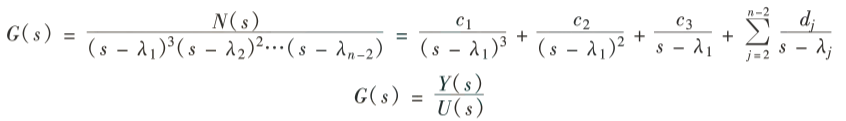
\includegraphics[width = .8\textwidth]{note/state space/figure/4.png}
        \end{center}

        此时有如下结果成立：
        \begin{center}
            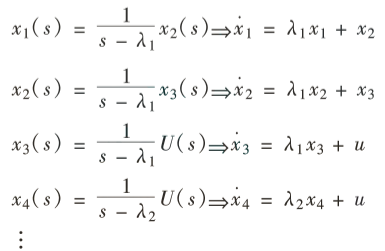
\includegraphics[width = .4\textwidth]{note/state space/figure/5.png}
        \end{center}

        可以写出系统状态方程如下：
        \begin{center}
            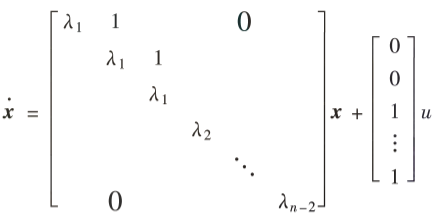
\includegraphics[width = .4\textwidth]{note/state space/figure/6.png}
        \end{center}

        系统输出方程如下：
        \begin{center}
            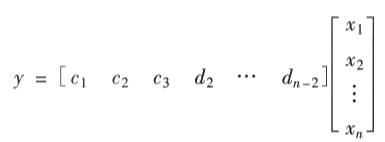
\includegraphics[width = .4\textwidth]{note/state space/figure/7.png}
        \end{center}

        \item 由高阶微分方程求状态空间表达式
        
        已知一个SISO系统，令y和u分别为其输出变量和输入变量，则输入输出间的动态关系可用一个高阶微分方程来表述，即：

        \begin{equation*}
            y^{(n)} + a_{n-1} y^{(n-1)} + \cdots + a_1 y^{(1)} + a_0 y = b_m u^{(m)} + b_{(m-1)} u^{(m-1)} + \cdots + b_1 u^{{1}} + b_0 u
        \end{equation*}

        假设系统初始条件为0，将上式两边进行Laplace变换，可得系统的传递函数：
        \begin{equation*}
            \frac{Y(s)}{U(s)} = \frac{b_m s^m + b_{m-1} s^{m-1} + \cdots +b_1 s +b_0}{s^n + a_{n-1} s^{n-1} + \cdots + a_1 s + a_0}
        \end{equation*}

        \begin{center}
            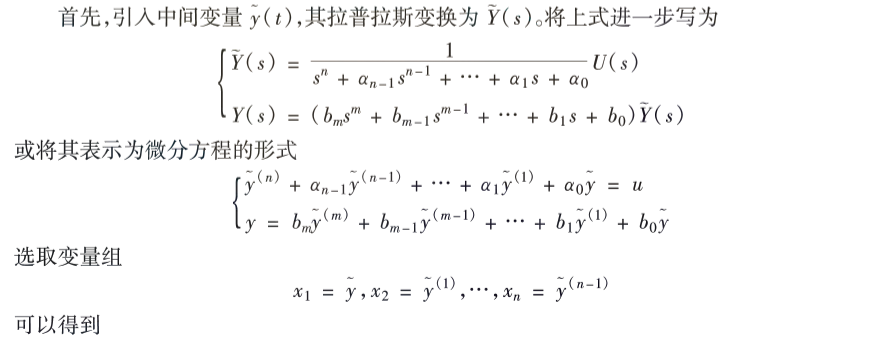
\includegraphics[width = .8\textwidth]{note/state space/figure/8.png}
        \end{center}

        \begin{center}
            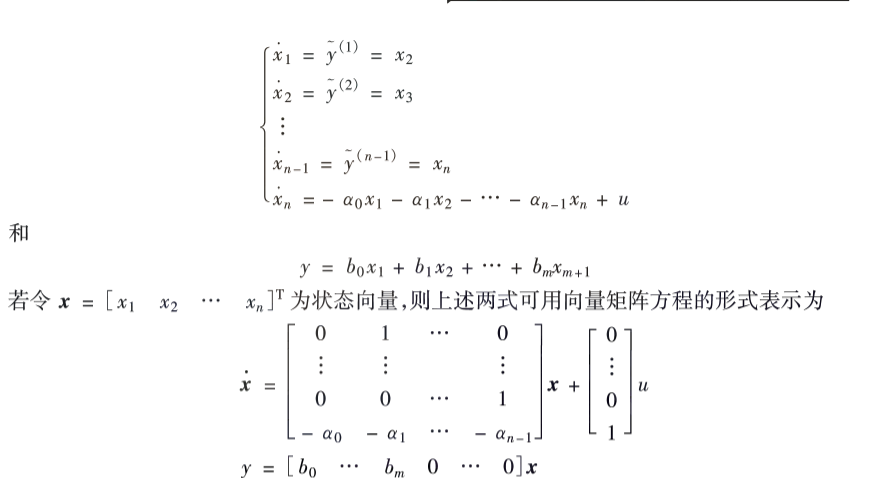
\includegraphics[width = .8\textwidth]{note/state space/figure/9.png}
        \end{center}
        
        如果该微分方程输出次数与输入相同，则传递函数可以拆成常数与一个分式之和，之后转化为上面的情况
    \end{itemize}

\end{enumerate}

\subsection{线性系统的代数等价}
\subsubsection{化状态空间为传递函数矩阵}

对于线性定常系统
\begin{equation*}
    \begin{cases}
        \dot{\bm{x}} = A \bm{x} + B \bm{u} \\
        \bm{y} = C \bm{x} + D \bm{u} 
    \end{cases}\quad t\geq t_0
\end{equation*}

对此式做Laplace变换，可导出
\begin{equation*}
    \begin{cases}
        s\bm{X}(s) = A \bm{X}(s) + B \bm{U}(s) \\
        \bm{Y} (s) = C \bm{X}(s) + D \bm{U}(s)  
    \end{cases}
    \Rightarrow 
    \begin{cases}
        \bm{X} (s) = (sI-A)^{-1} B\bm{U}(s) \\
        \bm{Y} (s) = [C (sI-A) ^{-1}B + D]U(s)
    \end{cases}
\end{equation*}

由此可以求出传递函数矩阵：
\begin{equation*}
    G(s) = C(sI - A)^{-1} B + D
\end{equation*}

\subsubsection{线性定常系统的几个概念}

\begin{definition}
    对于上述系统而言，称满足
    \begin{equation*}
        rank[sI-A \quad B] <n
    \end{equation*}

    的s为系统的输入解耦零点，称满足
    \begin{equation*}
        rank\left[
            \begin{array}{c}
                sI-A \\ C
            \end{array}
        \right]<n
    \end{equation*}

    的s为系统的输出解耦零点，称满足
    \begin{equation*}
        rank\left[
            \begin{array}{cc}
                sI-A & -B \\
                C & D \\
            \end{array}
        \right] <n + \min \{r,m\}
    \end{equation*}

    的s为系统的传输零点
\end{definition}

\subsubsection{代数等价系统}
\begin{definition}[代数等价]
    考虑两个同维数的线性定常系统：
    \begin{equation*}
        \begin{split}
            L:&\begin{cases}
                \dot{\bm{x}} = A \bm{x} + B \bm{u} \\
                    \bm{y} = C \bm{x} + D \bm{u} 
        \end{cases}\\
        L':&    \begin{cases}
        \dot{\overline{\bm{x}}} = \overline{A} \overline{\bm{x}} + \overline{B} \bm{u} \\
        \bm{\overline{y}} = \overline{C} \overline{\bm{x}} + \overline{D} \bm{u} 
    \end{cases}
        \end{split}
    \end{equation*}

    如果存在一个适当阶的定常可逆矩阵$P$，使得系统$L$和$L'$的系统参数矩阵满足：
    \begin{equation*}
        \overline{A} = PAP^{-1} \quad \overline{B} = PB \quad \overline{C} = CP^{-1} \quad \overline{D} = D
    \end{equation*}

    则称系统$L$和$L'$是代数等价的
\end{definition}

\subsubsection{代数等价系统的性质}

\begin{property}
    代数等价系统具有以下性质：
    \begin{enumerate}
        \item 相互代数等价的线性定常系统具有相同的特征方程、特征方程和极点
        \item 相互代数等价的线性定常系统具有相同的传递函数或传递函数矩阵
        \item 相互代数等价的线性定常系统具有相同的输入解耦零点、输出解耦零点和传输零点
    \end{enumerate}
\end{property}

\section{线性时变系统的运动分析}

\subsection{运动分析的含义}

\subsubsection{线性系统的运动分析与解存在唯一性}

对于线性时变系统，描述系统运动过程的状态方程为：
\begin{equation*}
    \dot{\bm{x}} = A(t) \bm{x} + B(t) \bm{u}  \quad   \bm{x}(t_0) = \bm{x}_0 \quad t \geq t_0
\end{equation*}

而对应的线性定常系统的状态方程为：
\begin{equation*}
    \dot{\bm{x}} = A \bm{x} + B \bm{u}  \quad   \bm{x}(0) = \bm{x}_0 \quad t \geq 0
\end{equation*}

显然，只有当状态方程满足初始条件的解存在唯一时，对系统的运动分析才是有意义的。这就要求状态方程中的系数矩阵和输入函数满足一定的假设，才可以保证方程解的存在唯一性。对于时变系统而言，如果系统矩阵$A(t)$和$B(t)$的所有的元素在时间定义区间$[t_0,t_f]$上均为实值连续函数，而输入$\bm{u}(t)$的元在时间区间$[t_0,t_f]$上是连续实函数，这时状态方程的解存在唯一

\subsubsection{线性系统响应的特点}

显然，线性系统的一个基本特征是其满足叠加原理。

自由运动是系统没有外部作用时：
\begin{equation*}
    \dot{\bm{x}} = A(t) \bm{x} \quad \bm{x}(t_0) = \bm{x}_0 \quad t \geq t_0
\end{equation*}
的解，用$\bm{\phi}(t,t_0,\bm{x}_0,0)$来表示，其中的$0$表示输入为零，称为零输入响应。强迫运动则是系统在零初始条件下的强迫方程
\begin{equation*}
    \dot{\bm{x}} = A(t) \bm{x} + B(t) \bm{u}  \quad   \bm{x}(t_0) =  \quad t \geq t_0
\end{equation*}
的解，用$\bm{\phi}(t,t_0,0,\bm{u})$来表示，称为零状态响应。系统由初始状态和输入作用所引起的整体响应$\bm{\phi}(t,t_0,\bm{x}_0,\bm{u})$就是两者的叠加，即：
\begin{equation*}
    \bm{\phi}(t,t_0,\bm{x}_0,\bm{u}) = \bm{\phi}(t,t_0,0,\bm{u}) + \bm{\phi}(t,t_0,\bm{x}_0,0)
\end{equation*}
这样，线性系统的运动分析可以分为两部分进行，然后再进行叠加


\section{线性定常系统的分析}
\subsection{线性定常系统的响应}
考察上述系统的状态转移矩阵。由于系统矩阵为定常矩阵$A$，显然满足条件式，于是系统的状态转移矩阵具有如下形式：
\begin{equation*}
    \bm{\Phi}(t,t_0) = I +\int_{t_0}^t A(\tau) d\tau + \frac{1}{2!}[\int_{t_0}^t A(\tau) d\tau]^2 + \cdots = e^{\int_{t_0}^t A(\tau) d\tau} = e^{A(t-t_0)}
\end{equation*}
当$t_0 = 0$时，$e^{At}$的表达式可以写为：
\begin{equation*}
    e^{At} = \sum_{k=0}^\infty \frac{1}{k!} A^k t^k
\end{equation*}
上式称为矩阵$A$的矩阵指数函数，即线性定常系统的状态转移矩阵为矩阵指数函数形式。

下面给出线性定常系统响应的结论：
\begin{theorem}
    给定线性定常系统，则有：
    \begin{enumerate}
        \item 其零输入响应为：
        \begin{equation*}
            \bm{\phi}(t,t_0,\bm{x}_0,0) = e^{A(t-t_0)} \bm{x}_0
        \end{equation*}
        \item 其零状态响应为：
        \begin{equation*}
            \bm{\phi}(t,t_0,0,\bm{u}) = \int_{t_0}^t e^{A(t-\tau)} B \bm{u}(\tau) d\tau
        \end{equation*}
        \item 其整体的状态响应为：
        \begin{equation*}
            \bm{\phi}(t,t_0,\bm{x}_0,\bm{u}) = e^{A(t-t_0)} \bm{x}_0 + \int_{t_0}^t e^{A(t-\tau)} B \bm{u}(\tau) d\tau
        \end{equation*}
    \end{enumerate}
\end{theorem}

\subsection{矩阵指数函数}
\subsubsection{矩阵指数函数的性质}
矩阵指数函数满足以下性质：
\begin{enumerate}
    \item $e^{A0} = I$
    \item $\frac{d}{dt} e^{At} = A e^{At}$
    \item $e^{A(t+s)} = e^{At} e^{As}$
    \item $(e^{At})^{-1} = e^{-At}$
    \item 当矩阵$A,B$可交换时：$e^{(A+B)t} = e^{At} e^{Bt} = e^{Bt} e^{At}$
    \item 若矩阵$P$为可逆矩阵，且$A = PJP^{-1}$，则$e^{At} = P e^{Jt} P^{-1}$
\end{enumerate}
\subsubsection{矩阵指数函数的求取}

\noindent \textbf{1}根据定义用级数来求取

\noindent \textbf{2}基于约当分解求取

这种方法的基本思想是先对矩阵$A$进行约当分解，然后利用性质6求取$e^{At}$

首先设$A$具有互异特征值$\lambda_i,i=1,2\cdots,n$，$\bm{p}_i$为$A$的与$\lambda_i$相对应的特征向量，记
\begin{equation*}
    P = [\bm{p}_1 \quad \bm{p}_2 \quad \cdots \quad \bm{p}_n]
\end{equation*}
则：
\begin{equation*}
    e^{At} = P \text{diag}(e^{\lambda_1 t} \quad e^{\lambda_2 t} \quad \cdots e^{\lambda_3 t}) P^{-1}
\end{equation*}
一般情况下，矩阵$A$的约当分解为：
\begin{equation*}
    A = P \text{diag}[J_1\quad J_2 \quad \cdots J_l] P^{-1}
\end{equation*}
其中$J_i$为约当块，此时有：
\begin{equation*}
    e^{At} = P \text{diag}(e^{J_1 t} \quad e^{J_2 t} \quad \cdots e^{J_3 t}) P^{-1}
\end{equation*}
再结合以下命题即可求解$e^{At}$
\begin{proposition}
    设$J_i$为一$p_i$阶约当块，$\lambda_i$为其特征值，其形式为：
    \begin{center}
        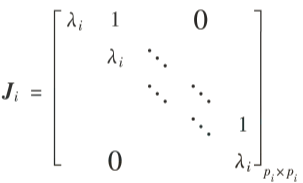
\includegraphics[width = .3\textwidth]{note/state space/figure/13.png}
    \end{center}
    则：
    \begin{center}
        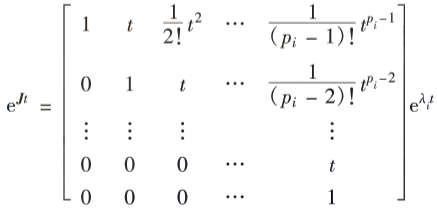
\includegraphics[width = .4\textwidth]{note/state space/figure/14.png}
    \end{center}
\end{proposition}

\noindent \textbf{3}利用Laplace变换求$e^{At}$
\begin{equation*}
    e^{At} = \mathcal{L}^{-1}[(sI - A)^{-1}]
\end{equation*}

证明从略

\noindent \textbf{4} 利用Cayley-Hamilton定理计算$e^{At}$

首先，先介绍一下Cayley-Hamilton定理
\begin{theorem}
    设$n$阶方阵$A$的特征方程为：
    \begin{equation*}
        f(\lambda) = \lambda^n + a_{n-1} s^{n-1} + \cdots + a_0 = 0
    \end{equation*}

    则方阵$A$满足$f(A) = 0$，即：
    \begin{equation*}
        A^n + a_{n-1} A^{n-1} + \cdots + a_0 = 0
    \end{equation*}
\end{theorem}

通过Cayley-Hamilton定理我们可以得到以下的结论：
\begin{center}
    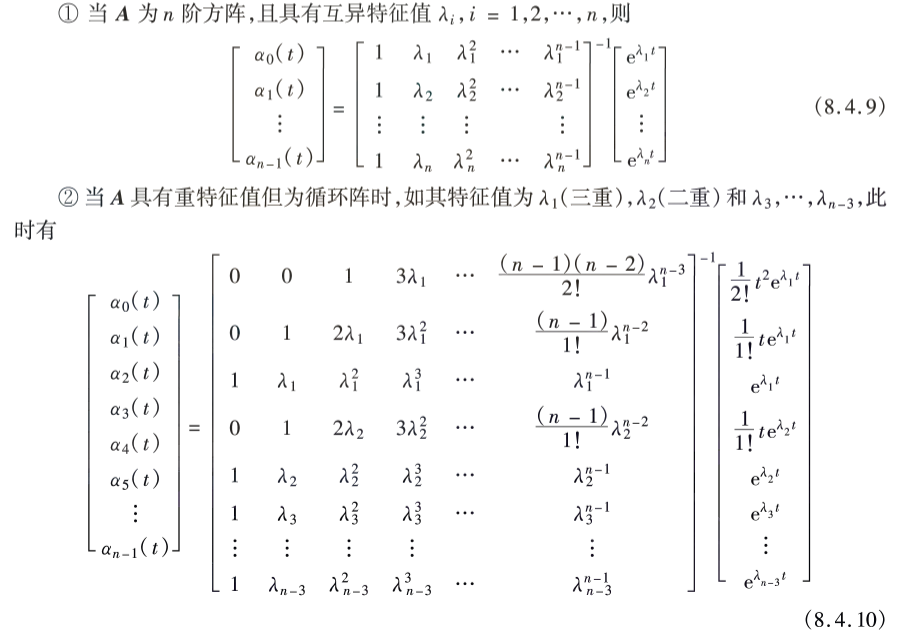
\includegraphics[width = \textwidth]{note/state space/figure/15.png}
\end{center}

\subsection{基于特征结构的状态响应表达}

假设系统矩阵$A$为$n$阶方阵，且其特征根两两相异：$\lambda_i \,(i=1,2,\cdots,n)$，假设每一个$\lambda_i$所对应的右特征向量为$v_i$，左特征向量为$w_i^T$，即：
\begin{equation*}
    A v_i = \lambda_i v_i \quad w_i^T A = w_i^T \lambda_i
\end{equation*}
则我们可以写出关于$A$的右特征向量矩阵与左特征向量矩阵：
\begin{equation*}
    P = [v_1,v_2,\cdots,v_n] \quad T = [w_1,w_2,\cdots,w_n]^T
\end{equation*}
则此时有以下两个式子成立：
\begin{equation*}
    \begin{split}
        e^{At} &= \sum_{i=1}^n v_i \overline{v_i}^T e^{\lambda_i t} \\
        &= \sum_{i=1}^n \overline{w_i} w_i^T e^{\lambda_i t}
    \end{split}
\end{equation*}
则此时我们可以写出这个表达式下的零输入响应与零状态响应：
\begin{equation*}
    \begin{split}
        x_{0u} = e^{At} x_0 &= \sum_{i=1}^n (v_i \overline{v_i}^T) x_0 e^{\lambda_i t} \\
        &= \sum_{i=1}^n (\overline{w_i} w_i^T) x_0 e^{\lambda_i t}
    \end{split}
\end{equation*}
\begin{equation*}
    \begin{split}
        x_{0x} &= \sum_{i=1}^n (v_i \overline{v_i}^T) \left[
            \sum_{j=1}^p b_j \int_0 ^t e^{\lambda_i (t-\tau)} u_j(\tau) d\tau
        \right]\\
        &= \sum_{i=1}^n (\overline{w_i} w_i^T) \left[
            \sum_{j=1}^p b_j \int_0 ^t e^{\lambda_i (t-\tau)} u_j(\tau) d\tau
        \right]
    \end{split}
\end{equation*}
其中$b_j$为B的第$j$列写状态方程组和输出方程组

\subsection{LTI系统的状态转移矩阵}

对于齐次状态方程，若有$x(t) = \Phi (t,t_0) x_0$，则称$\Phi(t,t_0)$为系统的状态转移矩阵。系统做自由运动时，它的运动形态唯一由状态转移矩阵决定，它包含了系统自由运动的全部信息

\begin{property}[状态转移矩阵的性质]
    \begin{enumerate}
        \item 状态转移矩阵的初始阵：$\Phi(0) = \Phi(t_0,t_0) = I$
        \item 状态转移矩阵的逆：$\Phi^{-1} (t,t_0) = \Phi(t_0,t)$
        \item 状态转移矩阵的传递性：$\Phi(t_2,t_1)\Phi(t_1,t_0) = \Phi(t_2,t_0)$
        \item 状态转移矩阵的导数：$\frac{d}{dt} \Phi(t,t_0) = A \Phi(t,t_0) = \Phi(t_0,t) A$
    \end{enumerate}
\end{property}

由上述信息可以写出系统状态响应与输出响应为：
\begin{equation*}
    \bm{x}(t) = \Phi(t,t_0)\bm{x}_0 + \int_{t_0}^t \Phi(t,\tau) B \bm{u}(\tau) d\tau
\end{equation*}
\begin{equation*}
    \bm{y}(t) = C \Phi(t,t_0) \bm{x}_0 +C \int_{t_0}^t \Phi(t,\tau) B \bm{u}(\tau) d\tau + D \bm{u}(t)
\end{equation*}

\section{离散系统状态空间分析}

\subsection{离散系统状态空间描述}

设线性离散系统的采样方式为周期采样，采样时刻为$kT,k\in N$，则状态空间描述为：
\begin{equation*}
    \begin{cases}
        \dot{\bm{x}}(k+1) = G(k)\bm{x}(k) + H(k) \bm{u}(k)\\
        \bm{y}(k) = C(k) \bm{x}(k) + D(k) \bm{u}(k)
    \end{cases}
\end{equation*}

其中$G,H,C,D$均为实矩阵，称$G(k)$为系统矩阵，$H(k)$为控制输入矩阵，$C(k)$为观测矩阵，$D(k)$为前馈矩阵。如果系统的参数矩阵均为定常的，即与采样时间标号$k$无关，则生疏式子可以化为以下式子：
\begin{equation*}
    \begin{cases}
        \dot{\bm{x}}(k+1) = G\bm{x}(k) + H \bm{u}(k)\\
        \bm{y}(k) = C \bm{x}(k) + D \bm{u}(k)
    \end{cases}
\end{equation*}

对于定常线性离散系统，我们称$G$的特征值为系统的特征值或极点。另外，类似于连续的情形，还有下述定义：
\begin{definition}
    对于上述线性定常离散系统，称满足
    \begin{equation*}
        rank[sI_n - G \quad H] < n
    \end{equation*}

    的$s$为系统的输入解耦零点，称满足
    \begin{equation*}
        rank \left[
            \begin{array}{c}
                sI_n - G \\    C
            \end{array}
        \right] <n
    \end{equation*}

    的$s$为系统的输出解耦零点，称满足
    \begin{equation*}
        rank \left[
            \begin{array}{cc}
                sI_n - G & -H \\
                C & D 
            \end{array}
        \right] < n+ min \{r,m\}
    \end{equation*}

    的s为系统的传输零点
\end{definition}

\subsubsection{离散系统状态空间的求法}

\noindent \textbf{1.}化差分方程为离散状态方程

这里假设差分方程中不含输入函数的高阶差分，即差分方程为：
\begin{equation*}
    y(k+n) + \sum_{i=1}^n a_i y(k+n-i) = b u(k)
\end{equation*}

选择状态变量为：
\begin{center}
    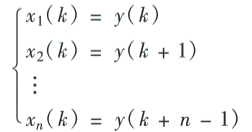
\includegraphics[width = .3\textwidth]{note/state space/figure/10.png}
\end{center}

则此时可以写出状态方程和输出方程为：
\begin{center}
    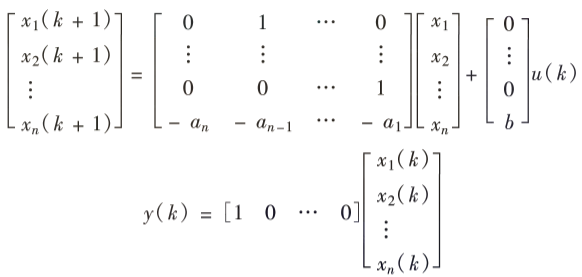
\includegraphics[width = .6\textwidth]{note/state space/figure/11.png}
\end{center}

\noindent \textbf{2.}化脉冲传递函数为离散状态方程

假设系统的脉冲传递函数$G(z)$分子分母多项式的阶数相同，且具有互不相同的实极点$z_1,\cdots,z_n$，则可以采用部分分式法将$G(z)$化为：
\begin{equation*}
    G(z) = \frac{\overline{y}(z)}{\overline{u}(z)} = d+ \sum_{i=1}^n \frac{k_i}{z-z_i}
\end{equation*}

上式中$\overline{y}(z),\overline{u}(z)$分别为输入输出的Z变换，$k_i = \text{Res}[G(z),z_i]$

取$\overline{x}_i(z) = \frac{1}{z-z_i} \overline{u}(z)$为离散状态变量的Z变换，则有：
\begin{equation*}
    z\overline{x}_i(z) = z_i \overline{x}_i(z) + \overline{u}(z)
\end{equation*}
\begin{equation*}
    \overline{y}(z) = d\overline{u}(z) + \sum_{i=1}^n k_i \overline{x}_i (z)
\end{equation*}

此时系统的状态方程和输出方程为：
\begin{center}
    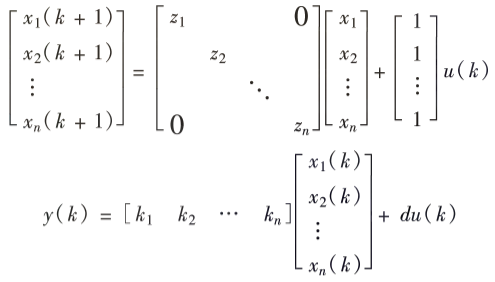
\includegraphics[width = .6\textwidth]{note/state space/figure/12.png}
\end{center}

\noindent \textbf{3.}线性连续系统状态方程的离散化

给定线性连续时变系统
\begin{equation*}
    \begin{cases}
        \dot{\bm{x}} = A(t) \bm{x} + B(t) \bm{u}  \quad t\in[t_0,t_a] \\
        \bm{y} = C(t) \bm{x} + D(t) \bm{u} \quad \bm{x}(t_0) = \bm{x}_0
    \end{cases}
\end{equation*}

则其离散化后的状态方程为：
\begin{equation*}
    \begin{cases}
        \bm{x}(k+1) = G(k) \bm{x}(k) + H(k) \bm{x}(k) \quad k = 0,1,\cdots,l \\
        \bm{y}(k) = C(k) \bm{x}(k) + D(k) \bm{u}(k) \quad \bm{x}(0) = \bm{x}_0
    \end{cases}
\end{equation*}

并且两者的系数矩阵间存在如下关系式：
\begin{equation*}
    \begin{split}
        G(k) &= \Phi[(k+1)T,kT] = \Phi(k+1,k) \\
        H(k) &= \int_{kT}^{(k+1)T} \Phi[(k+1)T,\tau]B(\tau) d\tau \\
        C(k) &= [C(t)]_{t=kT} \\
        D(k) &= [D(t)]_{t=kT} \\
    \end{split}
\end{equation*}

特别的，给定LTI系统
\begin{equation*}
    \begin{cases}
        \dot{\bm{x}} = A \bm{x} + B \bm{u} \quad \bm{x}(0) = \bm{x}_0 \\
        \bm{y} = C \bm{x} + D \bm{u}
    \end{cases}
\end{equation*}

的时间离散化模型可以写为：
\begin{equation*}
    \begin{cases}
        \bm{x}(k+1) = G \bm{x}(k) + H \bm{u}(k) \quad  \bm{x}(0) = \bm{x}_0 \\
        \bm{y}(k) = C \bm{x}(k) + D \bm{u}(k) \quad k = 0,1,2,\cdots
    \end{cases}
\end{equation*}

其中：
\begin{equation*}
    G = e^{AT} \qquad H = (\int_0^T e^{At} dt) B
\end{equation*}

这个系统的状态转移矩阵为：
\begin{equation*}
    \Phi(k) = G^k
\end{equation*}

\subsection{线性离散系统的运动分析}

\subsubsection{状态表达式的求解}

\noindent \textbf{1.}迭代法求状态表达式

对于上述提到的LTI系统而言，其状态运动的表达式为：
\begin{equation*}
    \bm{x}(k) = G^k \bm{x}_0 + \sum_{i=0}^{k-1} G^{k-i-1} H \bm{u}(i)
\end{equation*}

或
\begin{equation*}
    \bm{x}(k) = G^k \bm{x}_0 + \sum_{i=0}^{k-1} G^i H \bm{u}(k-i-1)
\end{equation*}

\noindent \textbf{2.}Z变换求状态表达式

对于上述LTI系统的状态差分方程而言，对其进行Z变换有：
\begin{equation*}
    z \bm{X}(z) - z\bm{x}_0 = G \bm{X}(z) + H \bm{U}(z)
\end{equation*}

故有：
\begin{equation*}
    \bm{x}(k) = Z^{-1}[\bm{X}(z)] = Z^{-1}[(zI - G)^{-1} (z \bm{x_0} + H \bm{U}(z))]
\end{equation*}

\subsubsection{状态转移矩阵的求法}

\noindent \textbf{1.}Z变换法

由上述两种求状态表达式的结果可以得到：
\begin{equation*}
    \Phi(k) = G^k = Z^{-1} [(zI - G )^{-1} z]
\end{equation*}

\noindent \textbf{2.}化矩阵$G$为标准型

首先讨论最特殊的情况：$G$的特征根没有重根

则此时我们可以取出其对应的右特征向量$P$，将$G$相似对角化为：
\begin{equation*}
    \varLambda = \text{diag}(\lambda_1,\lambda_2,\cdots,\lambda_n)
\end{equation*}

则此时我们可以求出状态转移矩阵为：
\begin{equation*}
    \Phi(k) = G^k = P \varLambda^k P^{-1} = P \text{diag}(\lambda_1^k,\lambda_2^k,\cdots,\lambda_n^k) P^{-1}
\end{equation*}

现在考虑$G$中特征根存在重根的情况，由于此时无法正常写出右特征向量矩阵，故此时将引入广义特征向量：
\begin{definition}[广义特征向量]
    矩阵$A$的广义特征向量满足：
    \begin{equation*}
        (A - \lambda I)^k v = 0 \quad k\geq 1
    \end{equation*}
    但：
    \begin{equation*}
        (A - \lambda I)^{k-1} v \neq 0 
    \end{equation*}
    广义特征向量可以组成一个向量链，设$\{P_1,P_2,\cdots,P_s\}$时对应于特征值$\lambda$的广义特征向量链，则这个向量链满足以下式子：
    \begin{equation*}
        \begin{cases}
            (A - \lambda I) P_1 = 0 \quad \text{（$P_1$是普通特征向量）}  \\
            (A - \lambda I) P_2 = P_1 \\
            (A - \lambda I) P_3 = P_2 \\
            \vdots \\
            (A - \lambda I) P_s = P_{s-1}
        \end{cases}
    \end{equation*}
\end{definition}

此时利用广义特征向量的定义，我们可以写出矩阵$G$的右特征向量矩阵$Q$，并将$G$化为其约旦标准型：

\begin{equation*}
    J = \text{diag}(J_1,J_2,\cdots,J_m)
\end{equation*}

此时我们可以写出状态转移矩阵为：
\begin{equation*}
    \Phi(k) = G^k = Q J^k Q^{-1} = Q \text{diag}(J_1^k,J_2^k,\cdots,J_m^k) Q^{-1}
\end{equation*}

其中$J_i$为特征值$\lambda_i$所对应的约旦块

\noindent \textbf{3.}化为关于G的有限项

由Cayley-Hamilton定理我们知道$G$一定为其特征方程的一个解，此时我们可以离散虚体部分状态转移矩阵写为$G$的有限项求和，即：
\begin{equation*}
    \Phi(k) = \sum_{i=0}^{n-1} \alpha_i(k) G^i
\end{equation*}

其中$\alpha_i(k)$为待定系数，可以仿照连续系统来求

\section{能控性与能观性}

在现代控制理论中,能控性和能观测性是两个重要的概念,它们是最优控制和最优估计的理论基础,基本的概念如下:
\begin{definition}[能控性与能观性的概念]
    \begin{itemize}
        \item 能控性是控制作用输入$u(t)$支配系统的状态向量$x(t)$的能力
        \item 能观测性是系统的输出$y(t)$反映系统的状态向量$x(t)$的能力
    \end{itemize}
    
    前者回答了$u(t)$能否使$x(t)$做任意转移的问题,后者则是回答了能否通过系统的输出量$y(t)$确定系统状态$x(t)$的问题
\end{definition}

\subsection{连续系统的能控性}

系统的能控性本质是在回答一个问题:已知某系统的当前时刻及其状态,是否存在一个容许控制,使得系统在该控制的作用下于有限时间后达到某个希望的特定状态?

由此,我们可以引出能控状态与系统的能控性的定义:
\begin{definition}[能控状态]
    对于线性定常系统,如果存在一个时刻$t_1 > 0$和一个无约束的容许控制$u(t),\quad t \in \left[0,t_1\right]$,使得系统在这个控制的作用下,系统由$x_0$出发经过时间$t_1$后由$x_0$转移到$x(t_1) = 0$,则称此$x_0$是系统的一个能控状态
\end{definition}

\begin{definition}[系统的能控性]
    对于线性定常系统,如果状态空间中的所有非零状态都是能控状态,则称该系统是能控的
\end{definition}

显然:时变系统的能控性和系统初始状态有关,而定常线性系统的能控性与初始时刻无关.

对于以上的定义,有几点需要注意:
\begin{enumerate}
    \item 能控性是一种定性性质,不涉及实现所需控制的具体方式
    \item 对定常系统,能控与否与$t_0$无关,与时间区间$\left[ t_0,t_1 \right]$无关,而对于时变系统,能控性与$t_0$和时间区间均有关
    \item 能控性只由系统的参数决定,因此是系统的固有属性
    \item 状态转移的轨迹没加以限制和规定,能控性是表征系统状态运动的一个定性特征
    \item 对线性定常系统能控性和能达性事等价的,但是对于时变系统和离散系统则是不等价的
    \item 不特殊说明,系统可控性均指状态能控性,要与输出能控性相区别
\end{enumerate}

在上面的注意事项中出现了能达性这个概念,我们现在来介绍这个概念:
\begin{definition}[能达状态]
    对于线性定常系统,如果存在一个时刻$t_1 > 0$和一个无约束的容许控制$u(t),\quad t \in \left[0,t_1\right]$,使得系统在这个控制的作用下,由零初始状态出发经过时间$t_1$后转移到$x(t_1) = x_f$,则称此$x_f$是系统的一个能达状态
\end{definition}

\begin{definition}[系统能达]
    对于线性定常系统,如果状态空间中的所有非零状态都是能达状态,则称此系统是能达的
\end{definition}

\subsection{系统能控性判据}

我们可以通过以下的几种方式判断下面的线性定常系统的能控性
\begin{equation*}
    \dot{x}(t) = A x(t) + B u(t)
\end{equation*}

上面的系统中$x$为$n$维状态向量;$u$为$r$维输入向量;$A \in \mathbb{R}^{n \times n}$和$B \in \mathbb{R}^{n \times r}$分别为系统矩阵和输入矩阵,均为常矩阵

\begin{theorem}
    线性定常系统是能控的当且仅当存在时刻$t_1 > 0$,使Gram矩阵
    \begin{equation*}
        W_c(t_1) = \int_0^{t_1} e^{-At} B B^T e^{-A^T t} dt 
    \end{equation*}
    是非奇异的
\end{theorem}

\begin{theorem}
    线性定常系统能控的充分必要条件是
    \begin{equation*}
        rank\left[\begin{array}{cccc}
            B & AB & \cdots & A^{n-1}B
        \end{array}\right] = n
    \end{equation*}
    其中$n = dim A$,我们称上述矩阵为$Q_c$
\end{theorem}

\begin{theorem}[PBH判据]
    线性定常系统是能控的当且仅当系统矩阵$A$的所有特征值$\lambda_i$满足:
    \begin{equation*}
        rank\left[ \lambda_i I - A \quad B \right] = n \quad \forall i \leq n
    \end{equation*}
    或者可以等价表述为:
    \begin{equation*}
        rank \left[ sI - A \quad B \right] = n \quad \forall s \in \mathbb{C}
    \end{equation*}
\end{theorem}

但是可能有些系统本身比较复杂，我们需要采用非奇异状态变换将这个系统化成一个比较简单的系统，可以通过以下的定理描述对于非奇异线性变换后的系统与原系统能控性之间的联系：

\begin{theorem}
    给定线性定常系统，通过非奇异状态变换$x = P \bar{x}$后的系统为$\dot{x} = \bar{A} \bar{x} + \bar{B} u$，则有：
    \begin{equation*}
        \text{rank}\left[
            \begin{array}{cccc}
                \bar{B} & \bar{A}\bar{B} & \cdots & \bar{A}^{n-1} \bar{B}
            \end{array}
        \right] = \text{rank} \left[
            \begin{array}{cccc}
                B & AB & \cdots & A^{n-1} B
            \end{array}
        \right]
    \end{equation*}
    其中$n$为系统状态变量的维数
\end{theorem}

我们还可以通过矩阵的Jordan标准型来判断系统的能控性：
\begin{theorem}
    \begin{center}
        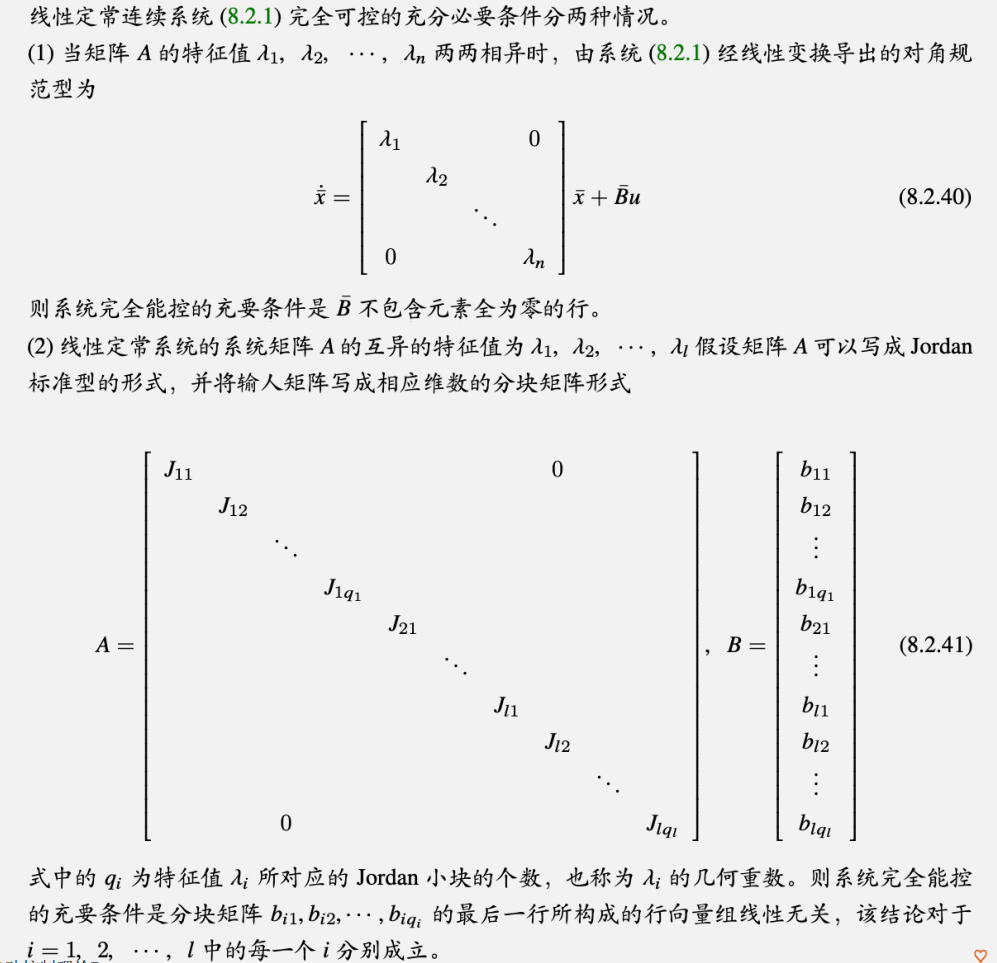
\includegraphics[width = .7\textwidth]{note/state space/figure/16.png}
    \end{center}
\end{theorem}

\subsection{连续系统的能观性}

和系统的能控性类似，我们可以给出系统能观性的概念：
\begin{definition}[能观状态]
    对于线性定常系统,如果对于初始时刻$t = 0$的一个非零初始状态$x_0$以及时间区间$\left[ 0,t_1 \right]$,使得由区间$[0,t_1]$上的系统输出$y(t)$可以唯一决定系统初始状态$x_0$,则称该状态$x_0$是能观的
\end{definition}

\begin{definition}[系统能观性]
    对于线性定常系统,如果状态空间中的所有非零状态都是能观状态,则称该系统是能观的
\end{definition}

同样的,时变系统的能观性依赖于初始时刻,而定长线性系统的能控性与能观性与初始时刻无关

\subsection{系统能观性判据}

我们可以通过以下的几种方式判断下面的线性定常系统的能观性:
\begin{equation*}
    \begin{split}
            \dot{x} &= A x\\
            y & = C x
    \end{split}
\end{equation*}

上面的系统中$x$为$n$维状态向量;$y$是$m$维输出向量;$A \in \mathbb{R}^{n \times n}$和$C \in \mathbb{R}^{m \times n}$分别为系统输入矩阵和系统输出矩阵,均为常矩阵

\begin{theorem}
    线性定常连续系统能观的充分必要条件是,存在有限时刻$t_1 > 0$,使Gram矩阵
    \begin{equation*}
        W_O(t_1) = \int_0^{t_1} e^{A^T t} C^T C e^{A t} dt
    \end{equation*}
    是非奇异的
\end{theorem}

\begin{theorem}
    线性定常系统能观的充分必要条件为:
    \begin{equation*}
        \text{rank} Q_O = \text{rank} \left[
            \begin{array}{c}
                C \\ CA \\ \vdots \\  C A^{n-1}
            \end{array}
        \right] = n
    \end{equation*}

    或者
    \begin{equation*}
        \text{rank} \left[
            \begin{array}{cccc}
                C^T & A^T C^T & \cdots & (A^T)^{n-1} C^T
            \end{array}
        \right] = n
    \end{equation*}
\end{theorem}

\begin{theorem}[PBH判据]
    线性定常系统完全能观的充分必要条件是,对矩阵$A$的所有特征值$\lambda_i,i \leq n$,均有:
    \begin{equation*}
        \text{rank}\left[
            \begin{array}{c}
                C \\ \lambda_i I - A
            \end{array}
        \right] = n
    \end{equation*}

    或者等价表述为:
    \begin{equation*}
        \text{rank} \left[
            \begin{array}{c}
                C \\ s I - A 
            \end{array}
        \right] = n \quad \forall s \in \mathbb{C}
    \end{equation*}
\end{theorem}

同样的，对于非奇异状态变换后的系统能观性与原系统能观性之间的联系，我们有以下的定理：
\begin{theorem}
    给定线性定常系统，通过非奇异状态变换$x = P \bar{x}$后的系统为
    \begin{equation*}
        \begin{split}
            \dot{x} &= \bar{A} x \\
            y &= \bar{C} x
        \end{split}
    \end{equation*}
    则有：
    \begin{equation*}
        \text{rank} \left[
            \begin{array}{c}
                \bar{C} \\ \bar{C} \bar{A} \\ \vdots \\ \bar{C} \bar{A}^{n-1}
            \end{array}
        \right] = \text{rank} \left[
            \begin{array}{c}
                C \\ C A \\ \vdots \\ C A^{n-1}
            \end{array}
        \right]
    \end{equation*}
    其中$n$为系统状态变量的维数
\end{theorem}

与能控性类似，也可以用系统的Jordan标准型来判断系统能观性：
\begin{theorem}
    \begin{center}
        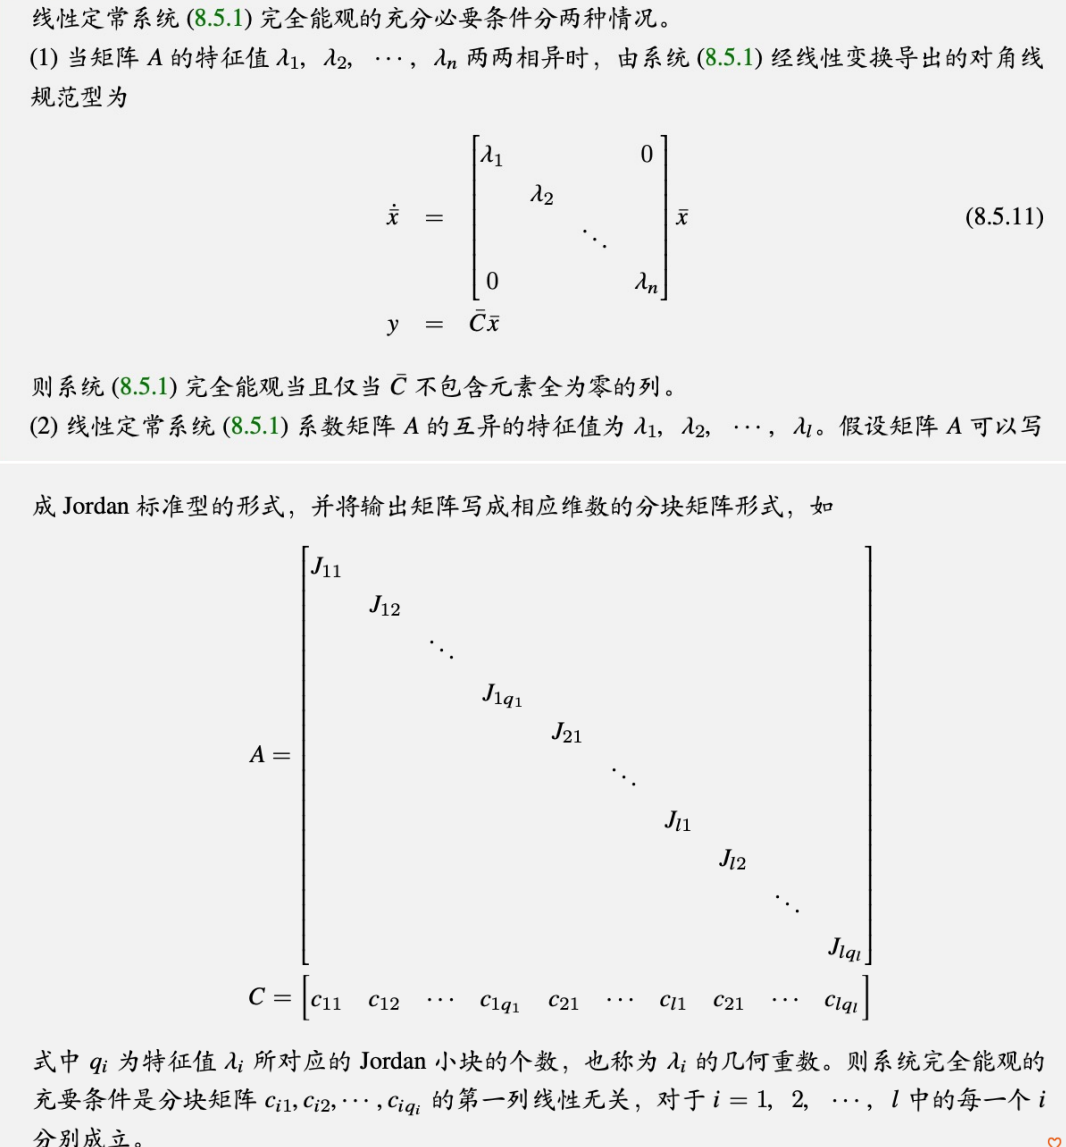
\includegraphics[width = .7\textwidth]{note/state space/figure/17.png}
    \end{center}
\end{theorem}

\subsection{连续系统结构分解}

\subsubsection{对偶性原理}
从上述能控性和能观性的定理和定义中可以看到，这两个概念是非常相似的，这两个概念在数学上是对称的，存在对偶性，我们可以通过下面的表为例：

\begin{center}
    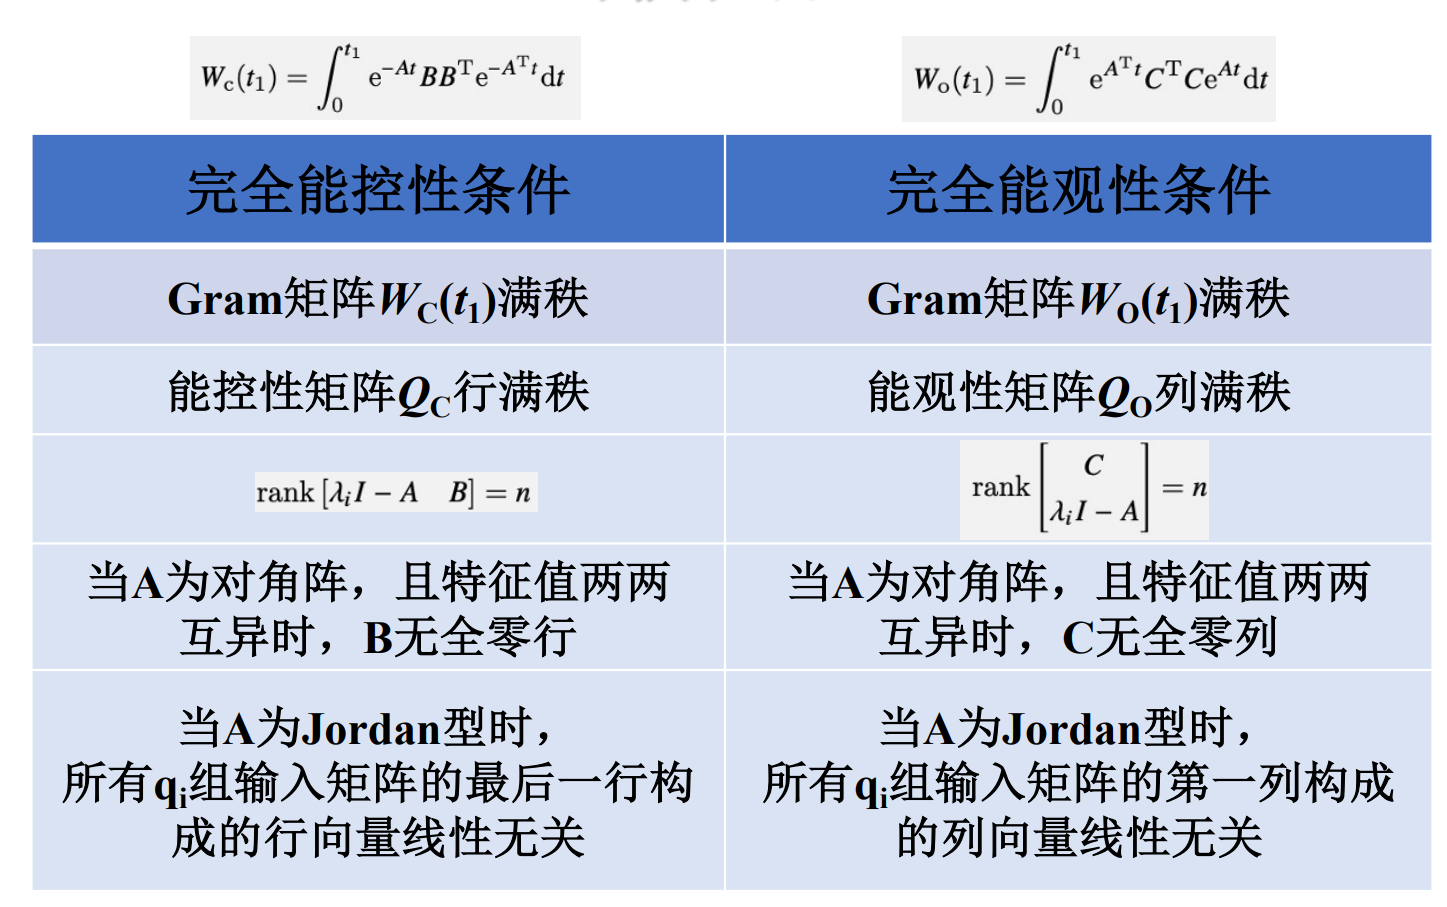
\includegraphics[width = .6\textwidth]{note/state space/figure/18.png}
\end{center}

\begin{definition}[对偶系统]
    线性定常系统
    \begin{equation*}
        \begin{cases}
            \dot{x} = A x + B u \\
            y = C x
        \end{cases}
    \end{equation*}
    的对偶系统为：
    \begin{equation*}
        \begin{cases}
            \dot{z} = A^T z + C^T v\\
            w = B^T z
        \end{cases}
    \end{equation*}

    由对偶性可以知道，如果原系统完全能控，则对偶系统完全能观；如果原系统完全能观，则对偶系统完全能控
\end{definition}

\subsubsection{能控规范型}

以下部分讨论的都是单输入单输出系统：
\begin{equation*}
    \begin{cases}
        \dot{x} = A x + b u \\
        y = C x
    \end{cases}
\end{equation*}
系统的特征多项式为：$\sum\limits_{i=0}^n \alpha_i s^i$，其中$\alpha_n = 1$，其能控性矩阵为:$Q_c = [
    \begin{array}{cccc}
        Ab & A^2 b & \cdots & A^{n-1} b
    \end{array}
]$

\begin{theorem}[第一能控性规范型]
    给定单输入单输出能控性系统，则在状态变换$x = Q_c \bar{x}$下，系统可转换为如下的第一能控规范型：
    \begin{equation*}
        \begin{cases}
            \dot{\bar{x}} = A_c \bar{x} + b_c u \\
            y = C_c \bar{x}
        \end{cases}
    \end{equation*}

    其中：
    \begin{equation*}
        \begin{split}
            A_c =  \begin{bmatrix}
            0 & \cdots & 0 & -\alpha_0 \\
            1 & \cdots & 0 & -\alpha_1 \\
              & \ddots & \vdots & \cdots \\
              & & 1 & -\alpha_{n-1} \\
        \end{bmatrix} , b_c = \begin{bmatrix}
            1 \\ 0 \\ \vdots \\ 0
        \end{bmatrix}  \\
        c_c = cQ_c = \begin{bmatrix}
            \beta_0 & \beta_1 & \cdots & \beta_{n-1} \\
        \end{bmatrix}\\
        \end{split}
    \end{equation*}
    \begin{equation*}
        \beta_i = c A^i b \quad \forall i < n
    \end{equation*}
\end{theorem}

\begin{theorem}[第二能控性规范型]
    给定单输入单输出能控性系统，其由特征多项式系数构成的Hankel矩阵$H_A$为：
    \begin{gather*}
        H_A = \begin{bmatrix}
            \alpha_1     & \alpha_2 & \cdots & \alpha_{n-1}  & 1       \\
            \alpha_2     & \alpha_3 & \cdots & 1             & 0       \\
            \vdots       & \vdots   & \ddots & \vdots        & \vdots  \\
            \alpha_{n-1} & 1        & \cdots & 0             & 0       \\
            1            & 0        & \cdots & 0             & 0       \\
        \end{bmatrix}
    \end{gather*}
    设其能控性矩阵为$Q_C$。令$P = Q_C H_A$，在状态变换$x = P \bar{x}$下，系统可转换为如下的第二能控规范型：
    \begin{equation*}
        \begin{cases}
            \dot{\bar{x}} = A_c \bar{x} + b_c u \\
            y = C_c \bar{x}
        \end{cases}
    \end{equation*}
    其中：
    \begin{gather*}
        A_C = \begin{bmatrix}
            0 & 1 & \cdots & 0 \\
            \vdots & \vdots &  & \vdots \\
            0 & 0 & \cdots & 1 \\
            -\alpha_0 & -\alpha_1 & \cdots & -\alpha_{n-1}
        \end{bmatrix} , \,
        b_c = \begin{bmatrix}
            0 & 0 & \cdots & 1 \\
        \end{bmatrix}^T  \\
        C_c = C P = \begin{bmatrix}
            \beta_0 & \beta_1 &  \cdots & \beta_{n-1}
        \end{bmatrix} \text{其中：}
        \begin{cases}
            \beta_{n-1} = C b \\
            \beta_{n-2} = C A b + \alpha_{n-1} C b \\
            \vdots \\
            \beta_1 = C A^{n-2} b + \alpha_{n-1} C A^{n-3} b + \cdots + \alpha_2 C b \\
            \beta_0 = C A^{n-1} b + \alpha_{n-1} C A^{n-2} b + \cdots + \alpha_1 C b \\
        \end{cases}
    \end{gather*}

    由第二能控标准型我们可以直接写出系统的闭环传递函数：
    \begin{gather*}
        D(s) = \frac{\sum\limits_{i=0}^{n-1} \beta_i s^i}{s^n + \sum\limits_{j=1}^{n-1} \alpha_i s^i}
    \end{gather*}
\end{theorem}

\subsubsection{能观规范型}

和能控规范型类似，以下部分讨论的都是单输入单输出系统：
\begin{equation*}
    \begin{cases}
        \dot{x} = A x + b u \\
        y = C x
    \end{cases}
\end{equation*}
系统的特征多项式为：$\sum\limits_{i=0}^n \alpha_i s^i$，其中$\alpha_n = 1$，其能观性矩阵为：$Q_O = \begin{bmatrix}
    C^T & A^T C^T & \cdots (A^T)^{n-1} C^T \\
\end{bmatrix}^T$

\begin{theorem}[第一能观规范型]
    给定单输入单输出能观性系统，则在状态变换$x = Q_O^{-1} \tilde{x}$下，系统可转换为如下第一能观规范型
    \begin{gather*}
        \dot{\tilde{x}} = \begin{bmatrix}
            0 & 1 & \cdots & 0 \\
            \vdots & \vdots & & \vdots \\
            0 & 0 & \cdots & 1 \\
            -\alpha_0 & -\alpha_1 &  \cdots & -\alpha_{n-1}
        \end{bmatrix} \tilde{x} + \begin{bmatrix}
            \beta_0 \\ \beta_1 \\ \vdots \\ \beta_{n-1}
        \end{bmatrix} u \\
        y = \begin{bmatrix}
            1 & 0 & \cdots & 0
        \end{bmatrix} \tilde{x}
    \end{gather*}

    其中：
    \begin{gather*}
        \beta_i = C A^i b\\
        b_O = Q_O b = \begin{bmatrix}
            \beta_0 \\ \beta_1 \\ \vdots \\ \beta_{n-1}
        \end{bmatrix}
    \end{gather*}
\end{theorem}

\begin{theorem}[第二能观规范型]
    给定单输入单输出能观性系统，其对应的Hankel矩阵为：
    \begin{gather*}
        H_A = \begin{bmatrix}
            \alpha_1     & \alpha_2 & \cdots & \alpha_{n-1}  & 1       \\
            \alpha_2     & \alpha_3 & \cdots & 1             & 0       \\
            \vdots       & \vdots   & \ddots & \vdots        & \vdots  \\
            \alpha_{n-1} & 1        & \cdots & 0             & 0       \\
            1            & 0        & \cdots & 0             & 0       \\
        \end{bmatrix}
    \end{gather*}
    令$Q = H_A Q_O$则在状态变换$x = Q^{-1} \tilde{x}$下，系统可转换为如下第二能观规范型：
    \begin{gather*}
        \dot{\tilde{x}} = \begin{bmatrix}
            0 & \cdots & 0 & -\alpha_0 \\
            1 & \cdots & 0 & -\alpha_1 \\
            \vdots & & \vdots & \vdots \\
            0 & \cdots & 1 & -\alpha_{n-1} 
        \end{bmatrix} \tilde{x} + \begin{bmatrix}
            \beta_0 \\ \beta_1 \\ \vdots \\ \beta_{n-1} \\
        \end{bmatrix} u  \\
        y = \begin{bmatrix}
            0 & \cdots & 0 & 1
        \end{bmatrix} \tilde{x}
    \end{gather*}
    其中：
    \begin{gather*}
        \begin{cases}
            \beta_{n-1} = C b \\
            \beta_{n-2} = C A b + \alpha_{n-1} C b \\
            \vdots \\
            \beta_1 = C A^{n-2} b + \alpha_{n-1} C A^{n-3} b + \cdots + \alpha_2 C b \\
            \beta_0 = C A^{n-1} b + \alpha_{n-1} C A^{n-2} b + \cdots + \alpha_1 C b 
        \end{cases}
    \end{gather*}
\end{theorem}

\subsubsection{能控性结构分解}

但是对于一个不完全能控的系统，其无法化为能控标准型，我们这时候应当如何提取出其中的能控部分，将能控部分和不能控部分分开呢？我们有以下的方式：

\begin{anymark}[能控性结构分解]
    给定一个$n$维线性定常系统，其能控性矩阵为$Q_C$，且有$\text{rank} Q_C < n$。$l_1 , l_2 , \cdots ,l_k$是$Q_C$列空间中$k$个线性无关的列向量，$l_{k+1},\cdots,l_n$是与向量组$\{l_1,l_2,\cdots,l_k\}$线性无关的$(n-k)$个线性无关的列向量，并令变换矩阵$P = \begin{bmatrix}
        l_1 & l_2 & \cdots & l_k & l_{k+1} & \cdots & l_n 
    \end{bmatrix}$。则状态变换$x = P \hat{x}$可将系统转化为按能控性分解的规范形式：
    \begin{gather*}
        \begin{cases}
            \begin{bmatrix}
                \dot{\hat{x}}_C \\ \dot{\hat{x}}_{\bar{C}}
            \end{bmatrix} = \begin{bmatrix}
                \hat{A}_C & \hat{A}_{12} \\
                0         & \hat{A}_{\bar{C}}\\
            \end{bmatrix} \begin{bmatrix}
                \hat{x}_C \\ \hat{x}_{\bar{C}}
            \end{bmatrix} + \begin{bmatrix}
                \hat{B}_C \\ 0
            \end{bmatrix} u \\
            y = \begin{bmatrix}
                \hat{C}_1 & \hat{C}_2
            \end{bmatrix} \begin{bmatrix}
                \hat{x}_C  \\  \hat{x}_{\bar{C}}
            \end{bmatrix}
        \end{cases}
    \end{gather*}
    并且有如下的结论成立：
    \begin{enumerate}
        \item $(\hat{A}_C,\hat{B}_C)$是完全能控的
        \item 子系统$\Sigma(\hat{A}_C,\hat{B}_C,\hat{C}_1)$的传递函数等于整个系统的传递函数，即：
        \begin{gather*}
            \hat{C}_1 (sI - \hat{A}_C)^{-1} \hat{B}_C = C (sI - A)^{-1} B
        \end{gather*}
        \item 两个子系统$\Sigma_1(\hat{A}_C,\hat{B}_C,\hat{C}_1),\Sigma_2(\hat{A}_{\bar{C}},\hat{B}_{\bar{C}},\hat{C}_2)$的特征多项式的乘积等于原系统的特征多项式\\
        其中两个子系统为：
        \begin{equation*}
            \begin{split}
                &\Sigma_1:\begin{cases}
                \dot{\hat{x}}_C = \hat{A}_C \hat{x}_C + \hat{A}_{12} \hat{x}_{\bar{C}} + \hat{B}_C u\\
                y_1 = \hat{C}_1 \hat{x}_C
                \end{cases} \\
                &\Sigma_2:\begin{cases}
                    \dot{\hat{x}}_{\bar{C}} = \hat{A}_{\bar{C}} \hat{x}_{\bar{C}} \\
                    y_2 = \hat{C}_2 \hat{x}_{\bar{C}}
                \end{cases}
            \end{split}
        \end{equation*}
        $\Sigma_1$为$k$维完全能控的子系统，$\Sigma_2$为$n-k$维不能控子系统，$y = y_1 + y_2$
    \end{enumerate}
    \begin{marker}
        对于一个不完全可控的系统，其能控性结构分解是不唯一的，因为不同的人取的$n$个线性无关的列向量不完全一样，导致变换矩阵$P$不相同
    \end{marker}
\end{anymark}

\subsubsection{能观性结构分解}

和上面类似，我们可以通过以下的方式将系统中的能观部分和不能观部分分开：
\begin{anymark}[能观性结构分解]
    给定$n$维线性定常系统，其能观性矩阵为$Q_o$，且有$\text{rank} Q_o = k < n$。$v_1^T,v_2^T,\cdots,v_k^T$是$Q_o$行空间中$k$个线性无关的行向量，$v_{k+1}^T,\cdots,v_n^T$是与向量组$\{v_1^T,v_2^T,\cdots,v_k^T\}$线性无关的$(n-k)$个线性无关的行向量，并令变换矩阵$P = \begin{bmatrix}
        v_1^T \\ v_2^T \\ \vdots \\ v_n^T
    \end{bmatrix}^T$，则线性变换$x = P^{-1} \hat{x}$将上述系统化为按能观性分解的规范型
    \begin{gather*}
        \begin{cases}
            \begin{bmatrix}
                \dot{\hat{x}}_o \\ \dot{\hat{x}}_o
            \end{bmatrix} = \begin{bmatrix}
                \hat{A}_o & 0 \\
                \hat{A}_{21} & \hat{A}_{\bar{o}}
            \end{bmatrix} \begin{bmatrix}
                \hat{x}_o \\ \hat{x}_{\bar{o}}
            \end{bmatrix} + \begin{bmatrix}
                \hat{B}_1 \\ \hat{B}_2
            \end{bmatrix} u\\
            y = \begin{bmatrix}
                \hat{C}_o & 0
            \end{bmatrix} \begin{bmatrix}
                \hat{x}_o \\ \hat{x}_{\bar{o}}
            \end{bmatrix}
        \end{cases}
    \end{gather*}
    并且有如下的结论成立：
    \begin{enumerate}
        \item $(\hat{A}_o, \hat{C}_o)$完全能观
        \item 子系统$\Sigma(\hat{A}_o,\hat{B}_1,\hat{C}_o)$的传递函数等于整个系统的传递函数，即：
        \begin{gather*}
            \hat{C}_o (sI - \hat{A}_o)^{-1} \hat{B}_1 = C (sI - A)^{-1} B
        \end{gather*}
        \item 两个子系统$\Sigma_1(\hat{A}_C,\hat{B}_C,\hat{C}_1),\Sigma_2(\hat{A}_{\bar{C}},\hat{B}_{\bar{C}},\hat{C}_2)$的特征多项式的乘积等于原系统的特征多项式\\
        其中两个子系统为：
        \begin{equation*}
            \begin{split}
                &\Sigma_1:\begin{cases}
                \dot{\hat{x}}_o = \hat{A}_o \hat{x}_o + \hat{B}_1 u\\
                y_1 = \hat{C}_o \hat{x}_o
                \end{cases} \\
                &\Sigma_2:\begin{cases}
                    \dot{\hat{x}}_{\bar{o}} = \hat{A}_{21} \hat{x}_o + \hat{A}_{\bar{o}} \hat{x}_{\bar{o}} + \hat{B}_2 u \\
                    y_2 = 0
                \end{cases}
            \end{split}
        \end{equation*}
        $\Sigma_1$为$k$维完全能观的子系统，$\Sigma_2$为$n-k$维不能观子系统，$y = y_1 + y_2$
    \end{enumerate}
\end{anymark}

\subsubsection{能控+能观结构分解}

此处考试不做要求，下面仅给出课上的ppt：
\begin{center}
    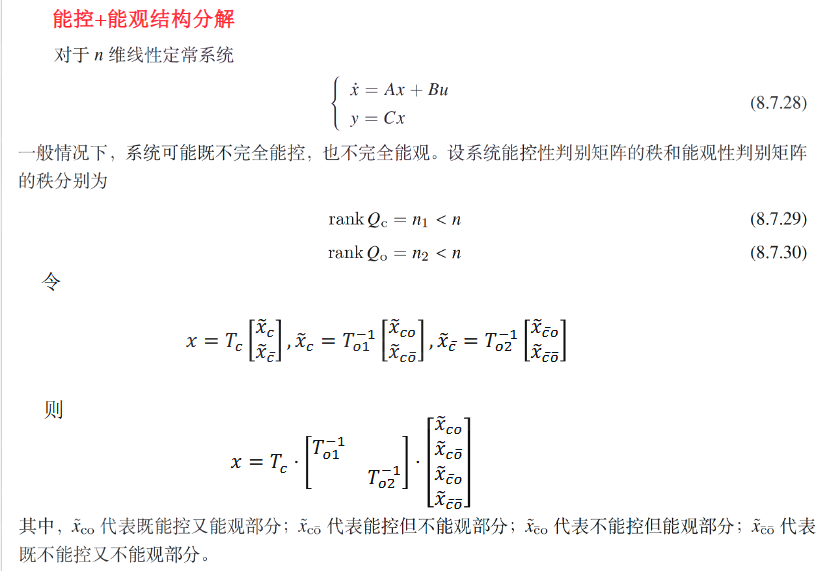
\includegraphics[width = .8\textwidth]{note/state space/figure/19.png} \\
    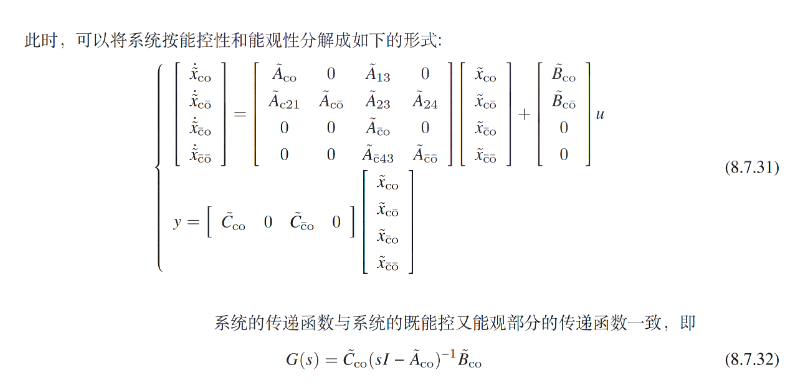
\includegraphics[width = .8\textwidth]{note/state space/figure/20.png}
\end{center}

\subsection{状态空间实现}

\subsubsection{能控能观性与零极点对消}

对于SISO系统，如果要通过秩判据一步一步判别系统的能控能观性，花费的精力会比较大，如果系统既是能控的也是能观的，我们有没有什么比较快的方法呢？

当然有！我们通过以下的定理来判别系统的能控能观性：
\begin{theorem}
    对于单输入单输出系统，一个传递函数的实现是能控能观的当且仅当传递函数无零极点对消
    \begin{marker}
        传递函数的实现指的是可以化成该传递函数的状态空间模型，注意在化成传递函数的过程中不要轻易约去分子分母的公因式！
    \end{marker}
\end{theorem}

\subsubsection{单输入单输出系统的实现}

对于一个单输入单输出系统，已知系统的传递函数，如果系统传递函数没有零极点对消，我们可以：
\begin{enumerate}
    \item 建立系统的能控规范型实现
    \item 建立系统的能观规范型实现
    \item 通过传递函数的部分分式展开，写出系统的Jordan标准型的实现形式
\end{enumerate}

\subsubsection{最小实现}

对于给定的传递函数矩阵，其实现并不唯一，其中维数最小的实现被称为最小实现。因此，最小实现是一种结构最简单的不可约实现。关于线性定常系统的最小实现有如下定理：
\begin{theorem}
    $G(s)$是一个严格真有理分实矩阵，实现$\Sigma(A,B,C)$是它最小实现的充要条件为：$(A,B)$能控，$(A,C)$能观  
\end{theorem}

\begin{theorem}
    $G(s)$任意两个最小实现$\Sigma_1(A_1,B_1,C_1)$和$\Sigma_2(A_2,B_2,C_2)$是代数等价的
\end{theorem}

那么怎么寻找最小实现呢？我们有以下的方式：
\begin{enumerate}
    \item 根据给定的传递函数矩阵$G(s)$，首先找出一种实现，为了使实现具有较低的维数，通常的做法是，当输入维数小于输出维数时，选择能控标准型实现，反之，选择能观标准型实现
    \item 对这个实现进行结构分解，其中既能控又能观的部分便是最小实现
\end{enumerate}


\begin{theorem}[能控标准型实现]
    模型
    \begin{equation*}
        \begin{cases}
            \dot{x} = Ax + Bu \\
            y = Cx
        \end{cases}
    \end{equation*}
    作为给定传递矩阵$ G(s) = \dfrac{\sum\limits_{i=0}^{n-1} P_i s^i}{s^n + \sum\limits_{j=0}^{n-1} \alpha_i s^i}$的一个能控标准型实现为
    \begin{equation*}
    \begin{cases}
        A = \begin{bmatrix}
        0_r & I_r & 0_r & \cdots & 0_r \\
        0_r & 0_r & I_r & \cdots & 0_r \\
        \vdots & \vdots & \vdots & & \vdots \\
        0_r & 0_r & 0_r & \cdots & I_r \\
        -\alpha_0 I_r & -\alpha_1 I_r & -\alpha_2 I_r & \cdots & -\alpha_{n-1} I_r
        \end{bmatrix} \in \mathbb{R}^{rn \times rn}
        \\[20pt]
        B = \begin{bmatrix}
        0_r \\
        0_r \\
        \vdots \\
        0_r \\
        I_r
        \end{bmatrix} \in \mathbb{R}^{rn \times r}
        \\[20pt]
        C = \begin{bmatrix}
        P_0 & P_1 & \cdots & P_{n-1}
        \end{bmatrix} \in \mathbb{R}^{m \times rn}
        \end{cases}
    \end{equation*}
    其中 $0_r$ 及 $I_r$ 分别为 $r \times r$ 零矩阵及 $r \times r$ 单位矩阵。
\end{theorem}


\begin{theorem}[能观标准型实现]
    模型
    \begin{equation*}
        \begin{cases}
            \dot{x} = Ax + Bu \\
            y = Cx
        \end{cases}
    \end{equation*}
    作为给定传递矩阵$ G(s) = \dfrac{\sum\limits_{i=0}^{n-1} P_i s^i}{s^n + \sum\limits_{j=0}^{n-1} \alpha_i s^i}$的一个能观标准型实现为
    \begin{equation*}
        \begin{cases}
        A = \begin{bmatrix}
        0_m & 0_m & \cdots & 0_m & -\alpha_0 I_m \\
        I_m & 0_m & \cdots & 0_m & -\alpha_1 I_m \\
        0_m & I_m & \cdots & 0_m & -\alpha_2 I_m \\
        \vdots & \vdots & & \vdots & \vdots \\
        0_m & 0_m & \cdots & I_m & -\alpha_{n-1} I_m
        \end{bmatrix} \in \mathbb{R}^{mn \times mn}
        \\[20pt]
        B = \begin{bmatrix}
        P_0 \\
        P_1 \\
        \vdots \\
        P_{n-1}
        \end{bmatrix} \in \mathbb{R}^{mn \times r}
        \\[20pt]
        C = \begin{bmatrix}
        0_m & 0_m & \cdots & 0_m & I_m
        \end{bmatrix} \in \mathbb{R}^{m \times mn}
        \end{cases}
    \end{equation*}
    其中 $0_m$ 及 $I_m$ 分别为 $m \times m$ 零矩阵及 $m \times m$ 单位矩阵。
\end{theorem}

\subsection{离散系统能控能观性}

\subsubsection{离散系统能控性}

对于离散系统我们考察以下定常线性离散时间系统的能控性：
\begin{gather*}
    x(k + 1) = G x(k) + H u(k)
\end{gather*}

\begin{definition}[能控状态]
    对于线性定常离散时间系统，如果存在一时刻$k_1 > 0$和一个无约束控制$u(k),k \in \mathbb{I}[0,k_1]$，使得系统在这个控制的作用下，系统由初始状态$x(0) = x_0$出发经过$k_1$步后转移到$x(k_1) = 0$，则称此状态$x_0$是系统的一个能控状态
\end{definition}

\begin{definition}[系统的能控性]
    对于线性定常离散时间系统，如果状态空间中的所有非零状态都是能控状态，则称该系统是能控的
\end{definition}

不过，在线性定常离散时间系统中，系统的能控性和能达性并不等价，我们给出以下的能达性的定义：
\begin{definition}[能达状态]
    对于线性定常离散时间系统，如果存在一时刻$k_1 > 0$，和一个无约束控制$u(k)$，使得系统在这个控制的作用下，系统由零初始状态$x(0) = 0$出发后转移到$x(k_1) = x_f$，则称此$x_f$是系统的一个能达状态
\end{definition}

\begin{definition}[系统能达性]
    对于线性定常离散时间系统，如果状态空间中的所有非零状态都是能达状态，则称该系统是能达的
\end{definition}

和连续系统类似，我们也可以给出离散系统中能控性和能达性的判据：

\begin{anymark}[能控性Gram判据]
    给定输入矩阵$H \in \mathbb{R}^{n \times r }$和非奇异系统矩阵$G \in \mathbb{R}^{n\times n}$，线性定常系统是能控的，当且仅当存在时刻$k_1 > 0$，使得Gram矩阵：
    \begin{gather*}
        W_c(k_1) = \sum_{i=0}^{k_1 - 1} G^{-1-i} H H^T (G^{-1-i})^T
    \end{gather*}
    是非奇异的
\end{anymark}

\begin{anymark}[能达性Gram判据]
    给定输入矩阵$H \in \mathbb{R}^{n \times r }$和非奇异系统矩阵$G \in \mathbb{R}^{n\times n}$，线性定常系统是能达的，当且仅当存在时刻$k_1 > 0$，使得Gram矩阵：
    \begin{gather*}
        W_c(k_1) = \sum_{i=0}^{k_1 -1} G^{k_1-1-i} H H^T (G^{k_1-1-i})^T
    \end{gather*}
    是非奇异的
\end{anymark}

\begin{anymark}[能控性和能达性的秩判据]
    给定输入矩阵$H \in \mathbb{R}^{n \times r }$和系统矩阵$G \in \mathbb{R}^{n\times n}$
    \begin{enumerate}
        \item 系统是\textbf{能达}的，当且仅当：
        \begin{gather*}
            \text{rank} \begin{bmatrix}
                H & GH & \cdots & G^{n-1} H
            \end{bmatrix} = n
        \end{gather*}
        \item 系统是\textbf{能控}的，当且仅当：
        \begin{gather*}
            \text{rank} \begin{bmatrix}
                H & GH & \cdots & G^{n-1} H
            \end{bmatrix} = \text{rank} \begin{bmatrix}
                H & GH & \cdots & G^{n-1} H & G^n
            \end{bmatrix}
        \end{gather*}
    \end{enumerate}
    观察以上两个判据，可以发现两个判据等价的充要条件为：\textbf{系统矩阵$G$是非奇异的}
\end{anymark}

\begin{theorem}[最小拍控制]
    考虑单输入离散时间线性时不变系统：
    \begin{equation*}
        x(k+1) = Gx(k) + hu(k), \quad k = 0, 1, \cdots
    \end{equation*}
    其中，$x$ 为 $n$ 维状态，$u$ 为标量输入，$G$ 和 $h$ 为 $n \times n$ 和 $n \times 1$ 常值矩阵，且设 $G$ 非奇异，那么，当系统为完全能控时，可构造如下一组控制输入：
    \begin{equation*}
        \begin{bmatrix}
        u(0) \\ u(1) \\ \cdots \\ u(n-1)
        \end{bmatrix}
        = -\bigl[ G^{-1}h,\ G^{-2}h,\ \cdots,\ G^{-n}h \bigr]^{-1} x_0
    \end{equation*}
    使系统必可在 $n$ 步内由任意非零初始状态 $x(0) = x_0$ 转移到状态空间原点。通常称这组控制为\textbf{最小拍控制}。
\end{theorem}

\subsubsection{离散系统能观性}

对于离散系统我们考察以下定常线性离散时间系统的能观性
\begin{gather*}
    \begin{cases}
        x(k+1) = G x(k) \\
        y(k) = C x(k)
    \end{cases}
\end{gather*}

\begin{definition}[能观状态]
    对于线性定常离散时间系统，如果对于初始时刻$k = 0$的一个非零的初始状态$x_0$，存在一个有限的时刻$k_1 > 0$，使得由区间$\mathbb{I}[0,k_1]$上的系统的输出$y(k)$可以唯一决定系统初始状态$x_0$，则称该状态$x_0$是能观的
\end{definition}

\begin{definition}[系统的能观性]
    对于线性定常离散时间系统，如果状态空间中的所有非零状态都是能观状态，则称该系统是能观的
\end{definition}

同样的，我们也可以给出离散系统中能观性判据：
\begin{anymark}[离散系统能观性Gram判据与秩判据]
    给定系统矩阵 $G \in \mathbb{R}^{n \times n}$ 和输出矩阵 $C \in \mathbb{R}^{m \times n}$，线性离散定常系统是能观的，当且仅当
    \begin{enumerate}
        \item \textbf{Gram判据}：存在有限时刻 $k_1 > 0$，使得 Gram 矩阵
        \begin{equation*}
            W_o(k_1) = \sum_{i=0}^{k_1} (G^{\mathrm{T}})^i C^{\mathrm{T}} C G^i
        \end{equation*}
        是非奇异的。
        \item \textbf{秩判据}：
        \begin{equation*}
            \mathrm{rank}\, Q_{od} = \mathrm{rank}
            \begin{bmatrix}
            C \\ CG \\ \vdots \\ CG^{n-1}
            \end{bmatrix} = n
        \end{equation*}
        或
        \begin{equation*}
            \mathrm{rank}
            \begin{bmatrix}
            C^{\mathrm{T}} & G^{\mathrm{T}}C^{\mathrm{T}} & (G^{\mathrm{T}})^2 C^{\mathrm{T}} & \cdots & (G^{\mathrm{T}})^{n-1} C^{\mathrm{T}}
            \end{bmatrix} = n
        \end{equation*}
    \end{enumerate}
\end{anymark}

\begin{theorem}[最小拍观测]
    考虑单输出离散时间线性时不变系统：
    \begin{align*}
        x(k+1) &= Gx(k), \quad x(0) = x_0, \quad k = 0, 1, 2, \cdots \\
        y(k) &= cx(k)
    \end{align*}
    其中 $x \in \mathbb{R}^n$，$y \in \mathbb{R}$，$G \in \mathbb{R}^{n \times n}$，$c \in \mathbb{R}^{1 \times n}$。那么，若系统完全能观测，则只利用 $n$ 步输出值 $y(0), y(1), \cdots, y(n-1)$ 就可构造相应初始状态 $x_0$：
    \begin{equation*}
        x_0 =
        \begin{bmatrix}
        c \\ cG \\ \vdots \\ cG^{n-1}
        \end{bmatrix}^{-1}
        \begin{bmatrix}
        y(0) \\ y(1) \\ \vdots \\ y(n-1)
        \end{bmatrix}
    \end{equation*}
\end{theorem}

\subsubsection{离散化系统对能控能观性的保持}

\begin{proposition}
    如果连续系统是不完全可控（不完全可观），则其离散化系统也是不能控（不能观）的
    \begin{proof}
        如果线性定常连续系统不能控，则其能控性矩阵
        \begin{equation*}
            Q_c = \begin{bmatrix} B & AB & \cdots & A^{n-1}B \end{bmatrix}
        \end{equation*}
        秩为 $\mathrm{rank}\,Q_c = k < n$，设列向量 $l_1, l_2, \ldots, l_k$ 是 $Q_c$ 中线性无关的列。

        对离散化系统，其能控性矩阵为：
        \begin{equation*}
            Q_{cd} = \begin{bmatrix} H & GH & \cdots & G^{n-1}H \end{bmatrix}
        \end{equation*}
        其中 $G = e^{AT},\ H = \left(\displaystyle\int_0^T e^{A\tau} d\tau\right) B$。

        通过 Cayley-Hamilton 定理：
        \begin{itemize}
            \item $\int_0^T e^{A\tau} d\tau$ 可表示为 $\{I, A, \cdots, A^{n-1}\}$ 的线性组合；
            \item 故 $H$ 可表示为 $\{B, AB, \cdots, A^{n-1}B\}$ 的线性组合；
            \item 进而 $H$ 的每列均可表示为 $l_1, l_2, \ldots, l_k$ 的线性组合。
        \end{itemize}

        对于 $GH$：
        \begin{equation*}
            GH = e^{AT} \int_0^T e^{At} B \,dt = \int_0^T e^{A(t+T)} B \,dt
        \end{equation*}

        同样通过 Cayley-Hamilton 可得：
        \begin{itemize}
            \item $GH$ 是 $\{B, AB, \cdots, A^{n-1}B\}$ 的线性组合；
            \item 所以 $GH$ 的每一列也可表示为 $l_1, l_2, \ldots, l_k$ 的线性组合。
        \end{itemize}

        类似地，所有 $G^{i-1}H$ 的每列也都可表示为这些列向量的线性组合。

        结论：
        \begin{equation*}
            \mathrm{rank}\,Q_{cd} \le k < n
        \end{equation*}
        即：离散化系统仍然不可控。对能观性也可以得出类似结论。

    \end{proof}
\end{proposition}

\begin{theorem}
    设系统
    \begin{gather*}
        \Sigma:\begin{cases}
            \dot{x} = A x + B u \quad x(0) = x_0 \\
            y = C x + D u \quad t \geq 0
        \end{cases}
    \end{gather*}
    能控或能观，令 $\lambda_1, \lambda_2, \cdots, \lambda_\mu$ 为 $A$ 的全部特征值，且当 $i \neq j$ 时有 $\lambda_i \neq \lambda_j$，则时间离散化系统 $\Sigma_T$ 保持能控或能观测的一个充分条件是，采样周期 $T$ 的数值对一切满足
    \begin{equation*}
        \mathrm{Re}|\lambda_i - \lambda_j| = 0 \qquad i, j = 1, 2, \cdots, \mu
    \end{equation*}
    的特征值，有
    \begin{equation*}
        T \neq \frac{2l\pi}{\mathrm{Im}(\lambda_i - \lambda_j)} \qquad l = \pm 1, \pm 2, \cdots
    \end{equation*}
\end{theorem}

\partsimage{cov18.pdf}
\part{系统的稳定性与分析}

\chapterimage{sd6.pdf}
\chapter{系统的稳定性}
\section{稳定性的基本概念}
\begin{definition}
    称系统是稳定的，当且仅当在扰动消除后，系统能够以足够的准确度恢复到原来的平衡状态，否则称系统是不稳定的
\end{definition}

\section{线性定常系统稳定的充要条件}
\begin{theorem}
    线性定常系统稳定的充要条件为：闭环系统特征方程的根全部具有负实部。或者说，闭环传递函数极点全部在S平面的左半平面
\end{theorem}

\section{Routh稳定判据}
\begin{definition}{Routh稳定判据}
    特征方程如果同时满足下面三个条件，闭环系统是稳定的：
    \begin{enumerate}
        \item 特征方程按降幂排列不存在缺项情况
        \item 特征方程的各项系数全是实数
        \item 用特征方程的各项系数排成Routh行列表，表中第一列各元全部大于零
    \end{enumerate}
\end{definition}
\begin{definition}
    Routh行列表如下：
    \begin{equation*}
        \begin{array}{cccccc}
            s^n & a_n& a_{n-2} & a_{n-4} & a_{n-6} & \cdots \\
            s^{n-1}&  a_{n-1} & a_{n-3} & a_{n-5} & a_{n-7} & \cdots \\
            s^{n-2} & b_1 & b_2 &b_3 & \cdots & \cdots \\
            \vdots  & c_1 & c_2 &c_3 & \cdots &\cdots \\
            s^2 & \vdots & \vdots & \vdots & \ddots & \\ 
            s^1 & \vdots & \vdots & \vdots & & \ddots \\
            s^0 & \vdots & \vdots & \vdots &\cdots & \cdots 
        \end{array}
    \end{equation*}
    
    其中：
    \begin{equation*}
        \begin{split}
            & b_1 = \frac{a_{n-1 }a_{n-2}-a_{n} a_{n-3}}{a_{n-1}} \\
            & b_2 = \frac{a_{n-1}a_{n-4}-a_n a_{n-5}}{a_{n-1}} \\
            & \vdots \\
            & c_1 = \frac{b_1 a_{n-3}- a_{n-1} b_2} {b_1} \\
            & c_2 = \frac{b_1 a_{n-5} - a_{n-1} b_3}{b_1}
        \end{split}
    \end{equation*}

    用文字表述如下：
    \begin{enumerate}
        \item 前两行：跳项写，缺项时写0
        \item 其他行计算（第i列）：取第i+1列与第一列做$2\times2$行列式然后除以上一行的第一项
    \end{enumerate}
    一些特殊情况的处理方法：
    \begin{enumerate}
        \item 上一行的第一项为0：将该项改为无穷小$\xi$，再做上述计算，最后取$\xi\rightarrow 0$的极限
        \item 若存在一行全零（全零行）：取全零行的上一行构造辅助方程，对该方程求导之后将对应系数填到该行中，再做上述计算
    \end{enumerate}
\end{definition}

\begin{property}
    Routh行列表具有以下性质：
    \begin{enumerate}
        \item 在计算Routh行列表时，用同一个正数去乘（或除）某一行的各元，不会影响稳定性判定结构。这样做往往能简化以后的运算
        \item Routh行列表第一列元自上而下符号改变的次数等于闭环系统特征方程中具有正实部根的个数（注：0不算改变符号！）
    \end{enumerate}
\end{property}

\begin{example}
    系统的特征方程为：
    \begin{equation*}
        D(s) = s^6 + 4s^5 - 4s^4 + 4s^3 - 7s^2 - 8s + 10 = 0
    \end{equation*}

    求该系统在右半平面特征根的数目

    \textbf{解}： 因为特征方程各项系数有正有负，所以系统不稳定。列Routh行列表：
    \begin{equation*}
        \begin{array}{cccccc}
            s^6 & 1             & -4 & -7 & 10 & \\
            s^5 & 4             & 4  & -8 & 0  & \\
            s^4 & -5            & -5 & 10 &    & \text{各元除以5}\\
                & -1            & -1 & 2  &    & \\
            s^3 & 0             & 0  &    &    & \text{做辅助方程}-s^4 -s^2 +2 = 0\\
                & -4            & -2 &    &    & \text{求导得}-4s^3 -2s = 0 \\
            s^2 & -\frac{1}{2}  & 2  &    &    & \text{各元同乘以2} \\
                & -1            & 4  &    &    &  \\
            s^1 & -18           &    &    &    &  \\
            s^0 & 4             &    &    &    &
        \end{array}
    \end{equation*}
    Routh行列表第一列两次变号，说明系统有两个特征根具有正实部。此外，解辅助方程$-s^4 -s^2 +2 = 0$，辅助方程的4个根为：$s_{1,2} = \pm \mathrm{j}\sqrt{2},s_{3,4} = \pm 1$，说明特征方程还有一对位于$S$平面虚轴上的纯虚根。
\end{example}

\section{求取保证系统稳定性的条件}

\subsection{确定某个参数的取值范围}

\begin{example}
    某控制系统的方框图如下图所示。已知参数$\zeta = 0.2,\omega_n = 86.6$试确定参数$K_1$取何值时系统方能稳定。
    \begin{center}
        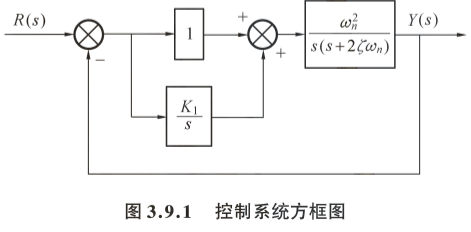
\includegraphics[width=.3\textwidth]{note/system stability/figure/1.png}
    \end{center}

    \textbf{解}： 图中闭环传递函数为：
    \begin{equation*}
        \varPhi(s) = \frac{Y(s)}{R(s)} = \frac{\omega_n^2(s+K_1)}{s^3 + 2\zeta\omega_n s^2 + \omega_n^2 s + K_1\omega_n^2}
    \end{equation*}

    由闭环传递函数求得系统的特征方程为：
    \begin{equation*}
        D(s) = s^3 +34.6 s^2 +7500 s +7500 K_1 = 0
    \end{equation*}

    列出相应的Routh行列表：
    \begin{equation*}
        \begin{array}{ccc}
            s^3 & 1 & 7500 \\
            s^2 & 34.6 & 7500 K_1 \\
            s^1 & \frac{34.6\times 7500 - 7500 K_1}{34.6} & 0 \\
            s^0 & 7500 K_1 & \\
        \end{array}
    \end{equation*}

    按照Routh行列表第一列各元全大于零的条件，应当满足下列不等式：
    \begin{equation*}
        \begin{split}
            \frac{34.6\times 7500 - 7500 K_1}{34.6} &>0 \\
            7500K_1 &>0
        \end{split}
    \end{equation*}

    故$0<K_1<34.6$
\end{example}

\subsection{确定某些参数间的相互关系}

\begin{example}
    单位负反馈系统的开环传递函数为：
    \begin{equation*}
        G(s) = \frac{K}{s(Ts+1)(2s+1)} \quad (K>0,T>0)
    \end{equation*}
    \begin{itemize}
        \item[(1)]为使闭环系统稳定，$K$和$T$应当满足什么关系？在$K-T$执教坐标系中画出使闭环系统稳定的区域。\\
        \textbf{解}：系统的特征方程为：
        \begin{equation*}
            D(s) = s(Ts+1)(2s+1) + K = 2Ts^3 +(2+T)s^2 +s +K =0
        \end{equation*}
        列出Routh行列表：
        \begin{equation*}
            \begin{array}{ccc}
                s^3 & 2T & 1 \\
                s^2 & 2+T & K \\
                s^1 & \frac{2+T-2KT}{2+T} & 0\\
                s^0 & K & \\
            \end{array}
        \end{equation*}

        由Routh行列表可知：$K< \dfrac{1}{T} + \dfrac{1}{2}$，画出$K-T$图如下：
        \begin{center}
            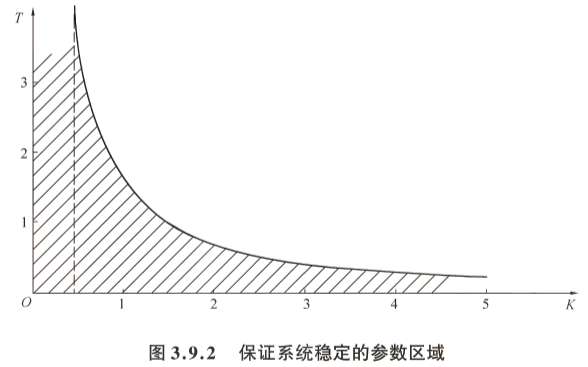
\includegraphics[width=.3\textwidth]{note/system stability/figure/2.png}
        \end{center}

        \item[(2)]若闭环系统处于临界稳定，持续振荡频率为1rad/s，求$K$和$T$的值\\
        \textbf{解}：若系统有频率为$\omega = 1$rad/s的持续振荡，说明系统的特征方程有一对纯虚根$\pm$j。根据特征方程出现纯虚根和Routh行列表的关系有：$K = \dfrac{1}{T}+\dfrac{1}{2}$。
        
        由$s^2$行得到辅助方程：
        \begin{equation*}
            (2+T)s^2 + K = 0
        \end{equation*}
        
        代入纯虚根可以解得：$T = \dfrac{1}{2},K=\dfrac{5}{2}$
    \end{itemize}
\end{example}

\subsection{保证系统稳定并且闭环极点远离虚轴}

\begin{example}
    系统方框图如下所示。要求闭环系统的特征根全在$s = -1 \pm j\omega$线左侧，试确定参数$K$的取值范围
    \begin{center}
        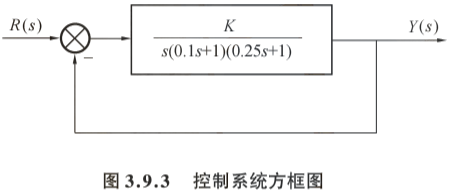
\includegraphics[width = .2\textwidth]{note/system stability/figure/3.png}
    \end{center}

    \textbf{解}：由方框图可以得到系统的特征方程为：
    \begin{equation*}
        s^3 + 14s^2 + 40s + 40K = 0
    \end{equation*}

    令$s = z - 1$，代入上式可得：
    \begin{equation*}
        z^3 + 11 z^2 + 15 z + (40K - 27) = 0
    \end{equation*}

    列出Routh行列表：
    \begin{equation*}
        \begin{array}{ccc}
            z^3 & 1 & 15 \\
            z^2 & 11 & 40K - 27 \\
            z^1 & \frac{11\times 155 - (40K-27)}{11} & 0 \\
            z^0 & 40K-27 & \\
        \end{array}
    \end{equation*}

    由Routh表可以得到以下不等式成立：
    \begin{equation*}
        \begin{split}
            11\times  15 -(40K-27) & >0 \\
            40K-27 &>0
        \end{split}
    \end{equation*}

    故$0.675<K<4.8$
\end{example}

\section{线性控制系统的稳态误差}

\subsection{控制系统的误差与稳态误差}

\begin{definition}{误差}
    在控制系统工作的时候，我们将期望的输出信号$y_r(t)$与实际的输出信号$y(t)$之差定义为\textbf{误差}，记为：
    \begin{equation*}
        e(t) \triangleq y_r(t)-y(t)
    \end{equation*}
\end{definition}

\begin{definition}{稳态误差}
    稳态误差的定义是误差信号的稳态值，记为：
    \begin{equation*}
        e_{ss} = \lim_{t\rightarrow \infty} e(t)
    \end{equation*}

    对于单位反馈系统，稳态误差可以由偏差信号的稳态值求得：
    \begin{equation*}
        e_{ss} = \lim_{t\rightarrow \infty} \varepsilon (t)
    \end{equation*}
\end{definition}

\subsection{终值定理和稳态误差的计算}

为了下面讨论问题方便，将单位反馈系统的开环传递函数写成典型环节形式：
\begin{equation*}
    G(s) = \frac{K\prod _{i=1}^m (\tau_i s + 1)}{s^v \prod_{j=1}^k (T_j s + 1) \prod _{k=1}^r (T_k^2 s^2 + 2\zeta_k T_k s + 1)}
\end{equation*}
其中$K$代表开环放大倍数，$v$代表开环传递函数中串联积分环节的个数

故此系统的稳态误差可以用Laplace变换的终值定理来求：
\begin{equation*}
    e_{ss} = \lim_{t\rightarrow \infty} e(t) = \lim_{s\rightarrow 0} s \varPhi_\varepsilon (s) R(s) = \lim_{s\rightarrow 0} s \frac{1}{1+G(s)} R(s) 
    = \lim_{s\rightarrow 0} s \frac{s^v \prod_{j=1}^q (\tau_j s + 1) \prod_{k=1}^r (T_k^2 s^2 + 2\zeta_k T_k s + 1)}{s^v \prod_{j=1}^q (T_j s + 1) \prod_{k=1}^r (T_k^2 s^2 + 2\zeta_k T_k s + 1) + K\prod_{i=1}^m (\tau_i s +1)} R(s)
\end{equation*}


由上式可以看出误差信号是与输入信号有关的，故下面将对不同的典型输入信号推导计算稳态误差：

\subsubsection{单位阶跃输入}

由上面可以知道：
\begin{equation*}
    e_{ss} = \lim_{t \rightarrow \infty}e(t) = \lim_{s\rightarrow 0} s E(s) = \lim_{s\rightarrow 0}s\frac{1}{1+G(s)}R(s) = \frac{1}{1+\lim_{s\rightarrow 0} G(s)}
\end{equation*}

观察到$e_{ss}$只与$\lim_{s\rightarrow 0} G(s)$有关，故定义静态位置误差系数：
$K_p = \lim_{s\to 0} G(s) = \begin{cases}
K&\quad v=0 \\
\infty &\quad v\geq 1
\end{cases}$


由上述定义可知单位阶跃作用下稳态误差的计算公式：
\begin{equation*}
    e_{ss} = \begin{cases}
        \frac{1}{1+K_p} &\quad v=0\\
        0 & \quad v\geq 1
    \end{cases}
\end{equation*}

\begin{definition}{系统的分类}
    开环传递函数终，串联积分环节数$v$对于控制系统的稳态误差起着重要的作用，为了区别各自特点，将系统根据$v$的值进行分类：
    \begin{enumerate}
        \item $v=0$：0型系统
        \item $v=1$：I型系统
        \item $v=2$：II型系统
        
        $\vdots$

        对于III型及以上的系统，使系统稳定是十分困难的，所以除非由特殊需要，一般很少采用III型及以上的控制系统
    \end{enumerate}
\end{definition}

\subsubsection{单位斜坡输入}

由上面可知稳态误差可以用下式计算：
\begin{equation*}
    e_{ss} = \lim_{s\to 0}s\frac{1}{1+G(s)} \frac{1}{s^2} = \lim_{s\to 0}\frac{1}{sG(s)}
\end{equation*}

定义$K_v$为系统的静态速度误差系数
\begin{equation*}
    K_v = \lim_{s\to 0} sG(s) = \begin{cases}
        0 & \quad v=0\\
        K & \quad v=1\\
        \infty & \quad v=2\\
    \end{cases}
\end{equation*}

代入上式可得：
\begin{equation*}
    e_{ss} = \begin{cases}
        \infty & \quad v=0\\
        \frac{1}{K_v} & \quad v=1\\
        0 & \quad v=2 \\
    \end{cases}
\end{equation*}

\subsubsection{单位加速度输入}
由上面可知稳态误差可以用下式计算：
\begin{equation*}
    e_{ss} = \lim_{s\to 0}s \frac{1}{1+G(s)} \frac{1}{s^3} = \lim_{s\to 0}\frac{1}{s^2 G(s)}
\end{equation*}

定义$K_a$为系统的静态加速度误差系
\begin{equation*}
    K_a = \lim_{s\to 0}s^2G(s) = \begin{cases}
        0 & \quad v=0\\
        0 & \quad v=1 \\
        K & \quad v=2\\
    \end{cases}
\end{equation*}

代入上式可得：
\begin{equation*}
    e_{ss} = \begin{cases}
        \infty & \quad v=0\\
        \infty & \quad v=1 \\
        \frac{1}{K_a} & \quad v=2\\
    \end{cases}
\end{equation*}

用一个表把上述三个信号作用下的稳态误差总结为：
\begin{center}
    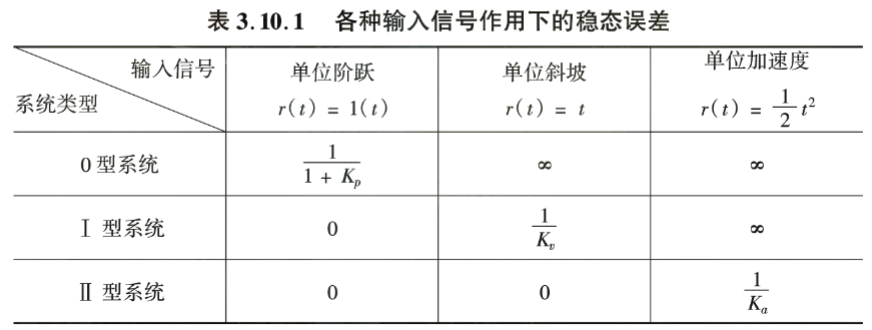
\includegraphics[width = .6\textwidth]{note/system stability/figure/4.png}
\end{center}

\subsection{干扰信号作用下的稳态误差}

主要思路：求出在$R(s) = 0$时由干扰信号引起的偏差函数$E_f(s) = \varPhi_{ef}(s)F(s)$，最后用终值定理即可求出由误差信号引起的偏差信号（单位反馈系统满足叠加定理）

\subsection{动态误差系数}

偏差信号的Laplace变换式为：
\begin{equation*}
    E(s) = \varPhi_e(s) R(s)
\end{equation*}

将偏差的闭环传递函数在$s=0$的邻域内展开成Taylor级数：
\begin{equation*}
    \varPhi_e(s) = \frac{1}{i!}\Sigma_{i=0}^\infty \varPhi_e^{(i)}(0) s^i
\end{equation*}

称$\dfrac{1}{i!}\varPhi_e^{(i)}(0)\quad (i\in Z)$为系统的动态误差系数

代入偏差信号的Laplace变换式后对其做Laplace反变换有：
\begin{equation*} 
    e_{ss}(t) = \frac{1}{i!}\Sigma_{i=0}^\infty \varPhi_e^{(i)}(0)r^{(i)}(t)
\end{equation*}

一种求动态误差系数的方法：一般$\varPhi_e(s)$为有理分式形式，对有理分式做大除法即可得到$\varPhi_e(s)$按s的升幂级数排列形式

\section{根轨迹法}

\subsection{基本概念}

考虑如图所示的闭环控制系统，其闭环传递函数为：
\begin{center}
    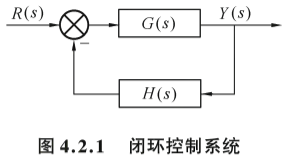
\includegraphics[width=.2\textwidth]{note/system stability/figure/5.png}
\end{center}
\begin{equation*}
    \varPhi(s) = \frac{Y(s)}{R(s)} = \frac{G(s)}{1+G(s)H(s)}
\end{equation*}

系统的特征方程为：$1+G(s)H(s) = 0$，将系统的开环传递函数写成如下零极点形式：
\begin{equation*}
    G(s)H(s) = \frac{k\prod_{i=1}^m (s-z_i)}{\prod_{j=1}^n (s-p_j)}
\end{equation*}

其中，$z_1,z_2,\cdots,z_m$和$p_1,p_2,\cdots,p_n$分别为系统的开环零点和极点，根据上述特征方程我们可以得到以下两个结论：
\begin{equation*}
    \begin{split}
        \left\lvert G(s)H(s) \right\rvert &= \frac{k\prod_{i=1}^m \left\lvert s-z_i \right\rvert }{\prod_{j=1}^n \left\lvert s-p_j \right\rvert } = 1 \\
        \angle G(s)H(s) &= \Sigma_{i=1}^m \angle(s-z_i) - \Sigma_{j=1}^n \angle(s-p_i) = \pm(2l+1)\pi \quad (l\in N)
    \end{split}
\end{equation*}

上述两式称为根轨迹方程，第一条称为根轨迹的幅值条件，第二条称为根轨迹的幅角条件

\begin{ascolorbox9}{画根轨迹的主要步骤}
    \begin{enumerate}
        \item 把系统的开环传递函数写成零极点形式
        \item 在$s$平面上画出开环零点和极点，一般用“$ \odot $”表示开环零点，用“$\times$”表示开环极点
        \item 在$s$平面上找出满足幅角条件的点，这些点连接成根轨迹。
        \item 对于根轨迹上的一些必要的点，利用幅值条件式求出他们所对应的$k$值，还可以进一步求出对应的开环放大倍数$K$
    \end{enumerate}
\end{ascolorbox9}

\subsection{绘制根轨迹的基本规则}

由上可知：负反馈闭环控制系统的特征方程为：
\begin{equation*}
    G(s) H(s) = -1
\end{equation*}

根轨迹的幅角条件为：
\begin{equation*}
    \angle G(s) H(s) = \Sigma_{i=1}^m \angle(s-z_i) - \Sigma_{j=1}^n \angle(s-p_j) = (2l+1)\pi
\end{equation*}

当根轨迹增益$k$由$0\to \infty$时，按照上述条件绘制的根轨迹称做负反馈根轨迹，或称根轨迹。利用下面的一些规则，可以在$s$平面上找到满足上述条件的点，从而绘制出根轨迹：
\begin{ascolorbox4}{根轨迹绘制八大法则}
    \begin{enumerate}
        \item \textbf{根轨迹的起点与终点}：根轨迹起始于开环极点，终止于开环零点；如果开环极点个数n大于开环零点个数m，则有n-m条根轨迹终止于无穷远处（无穷远点属于开环零点）
        \item \textbf{根轨迹的分支数，对称性和连续性}：根轨迹的分支数=开环极点数；根轨迹连续且对称于实轴
        \item \textbf{实轴上的根轨迹}：从实轴上最右端的开环零、极点算起，奇数开环零、极点到偶数开环零、极点之间的区域必是根轨迹（不区分该点是零点还是极点）

        以下图作为例子，红线部分为根轨迹：
        \begin{center}
            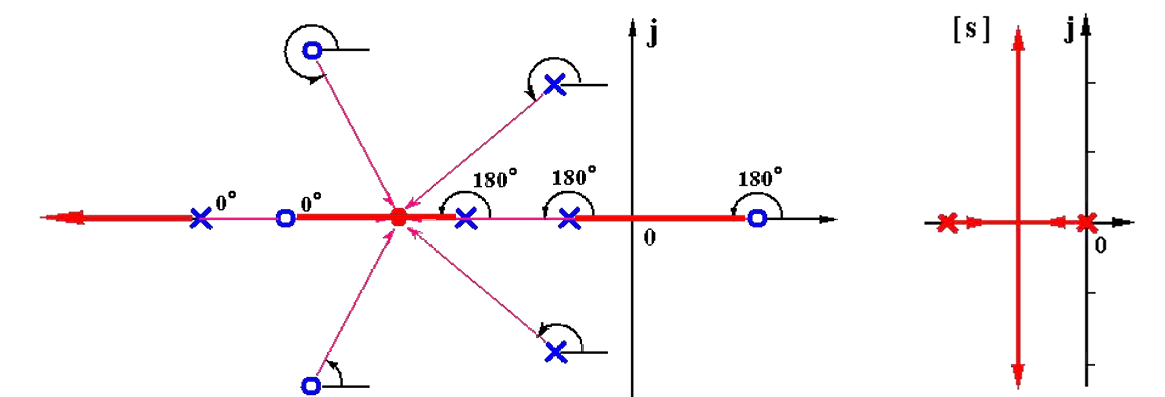
\includegraphics[width=.6\textwidth]{note/system stability/figure/6.png}
        \end{center}
        \item \textbf{闭环特征方程根之和}：当开环极点个数n与开环零点个数m之差大于2（n-m>2）时， 闭环特征方程根的和保持为一个常值，亦可写为：一部分根左移，另一部分根必然右移，且移动总量为0
        \item \textbf{根轨迹的渐近线}：当开环极点个数大于开环零点个数时，根轨迹的渐近线必定存在，且可用以下式子表示：
        \begin{equation*}
            \begin{split}
                \text{实轴截距：}& \sigma_a = \frac{\Sigma_{i=1}^n p_i - \Sigma_{j=1}^m z_j}{n-m} \\
                \text{倾斜角：}& \varphi_a = \frac{(2k+1)\pi}{n-m} \quad (k\in Z)
            \end{split}
        \end{equation*}
        \item \textbf{分离点求法}：设分离点为$d$（重根值），则分离点可由以下式子给出：
        \begin{equation*}
            \Sigma_{i=1}^n \frac{1}{d-p_i} = \Sigma_{j=1}^m \frac{1}{d-z_j}
        \end{equation*}
        \begin{equation*}
            \text{或}\frac{dD(s)}{ds} = 0 \text{的根}
        \end{equation*}
        \item \textbf{与虚轴交点的求法}：根轨迹与虚轴交点满足以下两个性质：
        \begin{itemize}
            \item[(I)] 该点时系统的临界稳定点
            \item[(II)] $s=j\omega \quad (\omega\in \mathbb{R})$ 
        \end{itemize}
        
        将上述两个性质任意一条代入闭环特征方程中即可求得根轨迹与虚轴交点
        \item \textbf{出射角/入射角（起始角/终止角）}：用幅角方程$\Sigma_{i=1}^m \angle(s-z_i) - \Sigma_{j=1}^n \angle(s-p_i) = \pm(2l+1)\pi$即可求得在起始点的幅角和终值点的幅角
        \item 定理（一种特殊情况）：若系统有2个开环极点，1个开环零点，且在复平面存在根轨迹，则复平面的根轨迹一定是以该零点为圆心的圆弧
    \end{enumerate}
\end{ascolorbox4}

\subsection{根轨迹法分析控制系统性能}
\begin{example}
    负反馈系统的开环传递函数为：
    \begin{equation*}
        G(s)H(s) = \frac{k(s+1)}{s(s-3)}
    \end{equation*}

    试用根轨迹分析该系统的性能

    \textbf{解}：给出的系统开环传递函数已是典型的零、极点形式，可以直接求出开环极点是$p_1 = 0,p_2 = 3,n=2$；开环零点是$z_1 = -1,m=1$

    同时可以求出分离点$d_1 = 1,d_2 = -3$；与虚轴交点$\pm j \sqrt{3}$，渐近线为实轴，画出根轨迹图如下：
    \begin{center}
        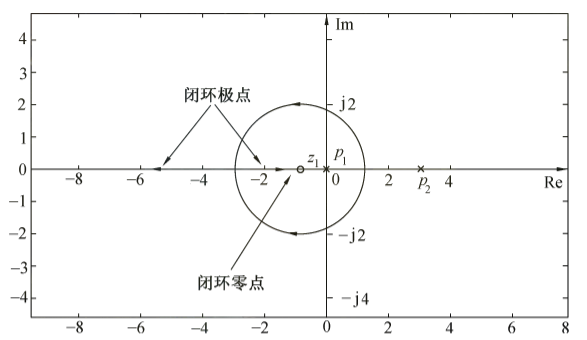
\includegraphics[width=.3\textwidth]{note/system stability/figure/7.png}
    \end{center}

    \begin{itemize}
        \item[(1)] 分析稳定性：该闭环负反馈系统，在开环放大倍数$K<1$时系统不稳定
        \item[(2)] 动态过程分析：根轨迹实轴上-3处回合分离点对应的$k=9$，开环放大倍数$K=3$。当$1<K<3$时，闭环传递函数有一对共轭的复数极点和一闭环极点$z_1 = -1$，系统是稳定的，但动态过程中会出现衰减振荡的分量；当$k>9,K>3$时，系统的闭环传递函数有两个负实数极点和一个零点$z_1=-1$，系统稳定，动态过程中无衰减振荡分量。由于系统的闭环传递函数中存在一个零点$z_1 = -1$和两个极点，所以需要用Laplace反变换或用MATLAB求取系统的阶跃响应曲线，再求出各项动态性能指标
        \item[(3)] 稳态误差分析：该系统的开环传递函数有一个$p_1 = 0$的极点，所以系统是I型系统。根据闭环极点的位置可以求出该店对应的$k$与$K$的值，开环放大倍数$K = K_v$，可以由此计算出稳态误差
    \end{itemize}
\end{example}

\subsection{特殊根轨迹}

\subsubsection{正反馈系统的根轨迹}
正反馈系统的特征方程为：
\begin{equation*}
    1-G(s)H(s) = 0
\end{equation*}

转化为幅值条件和相角条件为：
\begin{equation*}
    \begin{split}
        \left\lvert G(s)H(s)\right\rvert  &= \frac{k\prod_{i=1}^m\left\lvert (s-z_i)\right\rvert }{\prod_{j=1}^n \left\lvert (s-p_j) \right\rvert } = 1\\
        \angle G(s)H(s) &= \Sigma_{i=1}^m\angle(s-z_i) - \Sigma_{j=1}^n \angle(s-p_j) = 2l\pi
    \end{split}
\end{equation*}

因此，上述八大法则存在一定的偏差，不同之处为：
\begin{enumerate}
    \item 法则3：实轴上的根轨迹：从实轴上最右端的开环零、极点算起，偶数开环零、极点到奇数开环零、极点之间的区域必是根轨迹（不区分该点是零点还是极点）
    \item 法则5：渐近线的倾斜角：$\varphi_a = \dfrac{2l\pi}{n-m}$
    \item 法则8：入射角/出射角计算：$\Sigma_{i=1}^m\angle(s-z_i) - \Sigma_{j=1}^n \angle(s-p_j) = 2l\pi$
\end{enumerate}

\subsubsection{参数根轨迹}

绘制反馈系统的根轨迹时，其参变量并不一定是系统的开环增益。为了区别以开环增益为参变量的一般根轨迹，把以非开环增益的其他参数作为参变量的根轨迹称作\textbf{反馈系统的参数根轨迹}

计算此种形式的一般方法：构造“等效开环传递函数”，将参数根轨迹化为一般根轨迹
\begin{example}
    已知负反馈系统的开环传递函数为：
    \begin{equation*}
        G(s)H(s) = \frac{2}{s(\tau s + 1){s+1}}
    \end{equation*}

    试绘制以参数$\tau$为参变量的参数根轨迹。

    \textbf{解}：原系统的特征方程为：
    \begin{equation*}
        D(s) = s(\tau s +1)(s+1) + 2 = \tau s^2 (s+1) + s(s+1) + 2 = 0
    \end{equation*}

    构造开环传递函数：
    \begin{equation*}
        \overline{G}(s) \overline{H}(s) = \frac{\tau s^2 (s+1)}{s (s+1) + 2}
    \end{equation*}

    根据八大规则可以绘制根轨迹如下：
    \begin{center}
        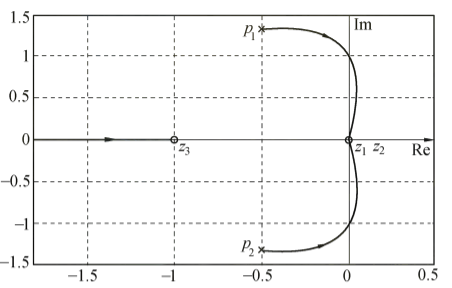
\includegraphics[width = .3\textwidth]{note/system stability/figure/8.png}
    \end{center}
\end{example}

\section{Nyquist稳定性判据}
在介绍Nyquist稳定判据前，我们先了解一个引理：
\begin{lemma}{对数留数定理}
    设$f(z)$在简单闭曲线$C$上处处解析且不等于0，在$C$内除去有限个极点$b_j(1\leq j \leq m)$外也处处解析，且在$C$内有零点$a_k(1\leq k \leq n)$，$\varphi(z)$在$C$上及内部均解析，则：
    \begin{equation*}
        \frac{1}{2\pi i}\oint_C \varphi(z) \frac{f'(z)}{f(z)}dz = \sum_{k=1}^n \alpha_k \varphi(a_k) -\sum_{j=1}^m \beta_j \varphi(b_j)
    \end{equation*}

    其中$\alpha_k$为$a_k$的阶数，$\beta_j$为$b_j$的阶数，$C$取正方向

    特别地，若$\varphi(z)\equiv 1$，有：
    \begin{equation*}
        \frac{1}{2\pi i} \oint_C \frac{f'(z)}{f(z)}dz = \sum_{k=1}^n \alpha_k  -\sum_{j=1}^m \beta_j = Z - P
    \end{equation*}

    其中，$Z$为$f(z)$在$C$内的零点总个数，$P$为$f(z)$在$C$内的极点总个数（均计算重数）

    上式中$\dfrac{1}{2\pi i}\displaystyle{\oint_C \frac{f'(z)}{f(z)}}$称为对数留数，其几何意义为：当点$z$沿$C$的正方向绕行一周后幅角$\Delta_C \arg f(z)$的改变量的$\dfrac{1}{2\pi}$倍，或$w = f(z)$在$w$平面内沿闭曲线$\Gamma_w$绕原点的圈数
\end{lemma}

此时我们就可以引出Nyquist稳定判据的定义：
\begin{definition}
    对于一个LTI系统，设$Z$为在右半平面中的闭环极点个数，$P$为在右半平面中的开环极点个数，$N$为s沿开环Nyquist曲线穿过$(-1,j0)$点左侧负实轴的次数，则有：
    \begin{equation*}
        Z = P - 2N
    \end{equation*}

    显然，当$Z=0$时系统是稳定的，$Z>0$时系统是不稳定的

    当开环系统中含有积分环节时，对应的Nyquist曲线需要从$\omega = 0$到$\omega=0^+$顺时针补充半径为$\infty$，角度为$v\times \dfrac{\pi}{2}$的圆弧
\end{definition}

注意到在上述定义中有涉及“穿越”，下面给出“穿越”的定义：
\begin{definition}
    对于Nyquist曲线，我们认为其从第二象限穿越$(-1,j0)$左侧负实轴至第四象限为正穿越，反之为负穿越

    半次穿越：Nyquist曲线起始或终止于$(-1,j0)$左侧负实轴，此时记穿越为半次穿越，正负值定义同上

    穿越的示意图如下所示：
    \begin{center}
        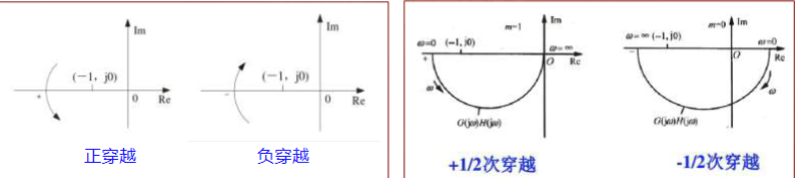
\includegraphics[width = .5\textwidth]{note/system stability/figure/9.png}
    \end{center}
\end{definition}

\begin{example}
    （此例题摘自上课ppt）
    \begin{center}
        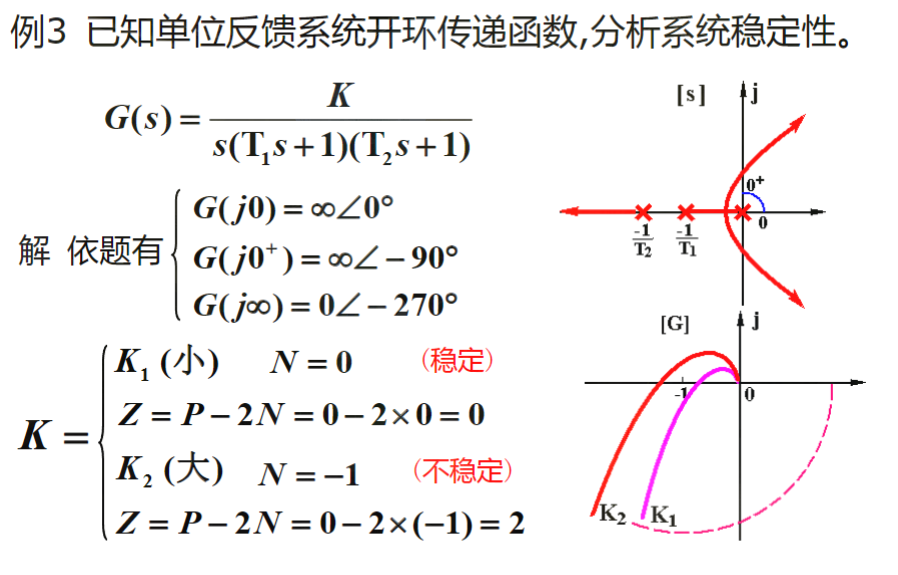
\includegraphics[width = .5\textwidth]{note/system stability/figure/10.png}
    \end{center}
\end{example}

\section{线性离散系统的稳定性}

\subsection{$s$平面到$z$平面的映射关系}

在定义Z变换时，我们定义了复变量$s$与复变量$z$之间的转换关系为：
\begin{equation*}
    z = e^{Ts}
\end{equation*}
将$s = \sigma + j \omega $带入可以得到：
\begin{equation*}
    z = e^{(\sigma + j \omega)T} = e^{\sigma T} e^{j\omega T} = \left\lvert z \right\rvert e^{j\omega T}
\end{equation*}
于是我们可以得到$s$平面到$z$平面的基本映射关系为：
\begin{equation*}
    \left\lvert z \right\rvert = e^{\sigma T} \quad \angle z = \omega T
\end{equation*}
观察上式可以得到：$s$平面的虚轴在$z$平面的映像为单位圆，$s$左半平面在$z$平面的映像为单位圆内，$s$右半平面在$z$平面的映像为单位圆外，具体如下图所示：
\begin{center}
    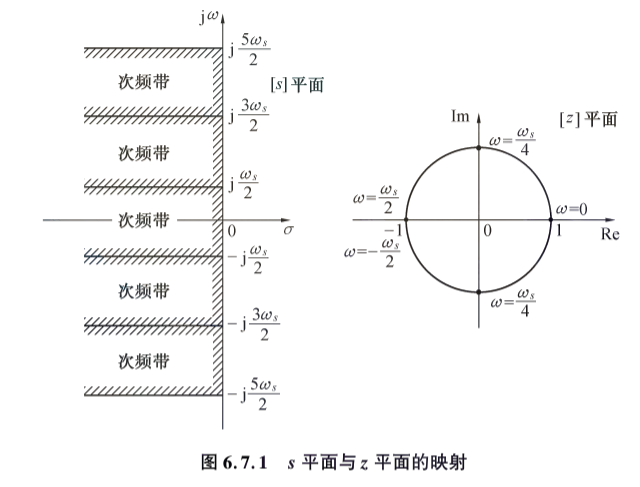
\includegraphics[width = .5\textwidth]{note/system stability/figure/11.png}
\end{center}

\subsection{线性离散系统稳定的充要条件}

首先，我们先假设闭环线性离散系统的特征方程的根，或闭环脉冲传递函数的极点为$z_1,z_2,\cdots,z_n$，则线性离散系统稳定性具有如下定理：
\begin{theorem}
    线性离散系统稳定的充要条件为：线性离散系统的全部特征根$z_i\, (i=1,2,\cdots,n)$都分布在$z$平面的单位圆内，或者说全部特征根的模都必须小于1，即：$\left\lvert z_i \right\rvert <1 \,(i=1,2,\cdots,n) $。如果在上述特征根中，有位于$z$平面单位圆之外者时，闭环系统将是不稳定的
\end{theorem}

\subsection{Routh稳定判据}

在线性离散系统中，判断稳定性需要判别特征方程的根是否在$z$平面的单位圆内，但是在连续系统中，Routh判据是判断极点是否在左半平面。故在线性离散系统中，不能直接使用Routh判据。为了使用Routh判据，需要将稳定区域映射到新平面的左半平面，故此时引入$w$变换，将$z$平面上单位圆内部区域，映射到$w$平面的左半平面，即：
\begin{equation*}
    w = \frac{z+1}{z-1}
\end{equation*}

两个平面间的映射关系由下图表示：
\begin{center}
    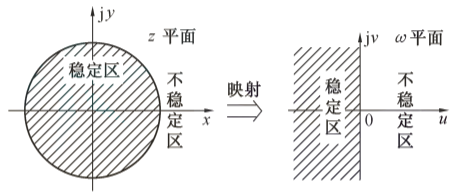
\includegraphics[width = .6\textwidth]{note/system stability/figure/12.png}
\end{center}

显然，$w$变换是线性变换的一种，且其可逆。$z$的有理多项式经过$w$变换之后，可以得到$w$的有理多项式。以$z$为变量的特征方程经过$w$变换之后得到以$w$为变量的特征方程，就可以应用Routh判据来判断线性离散系统的稳定性

\begin{example}[摘自课本例题6.7.3]
    \begin{center}
        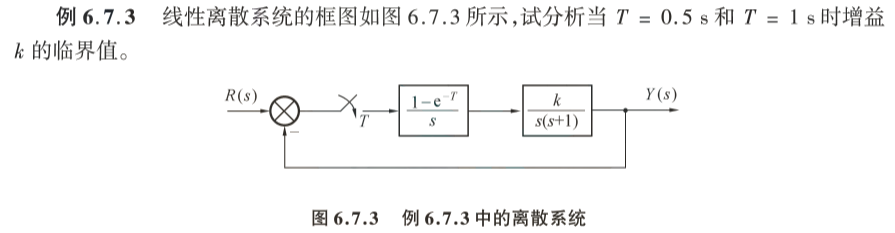
\includegraphics[width = .8\textwidth]{note/system stability/figure/13.png}\\
        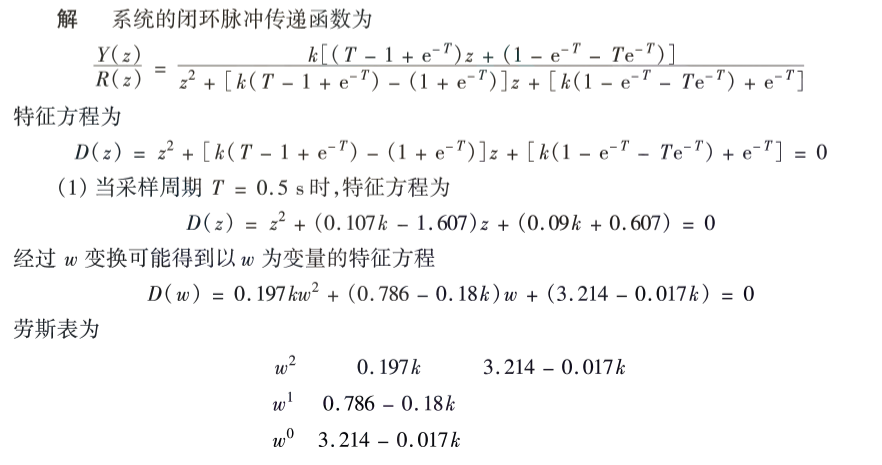
\includegraphics[width = .8\textwidth]{note/system stability/figure/14.png}\\
        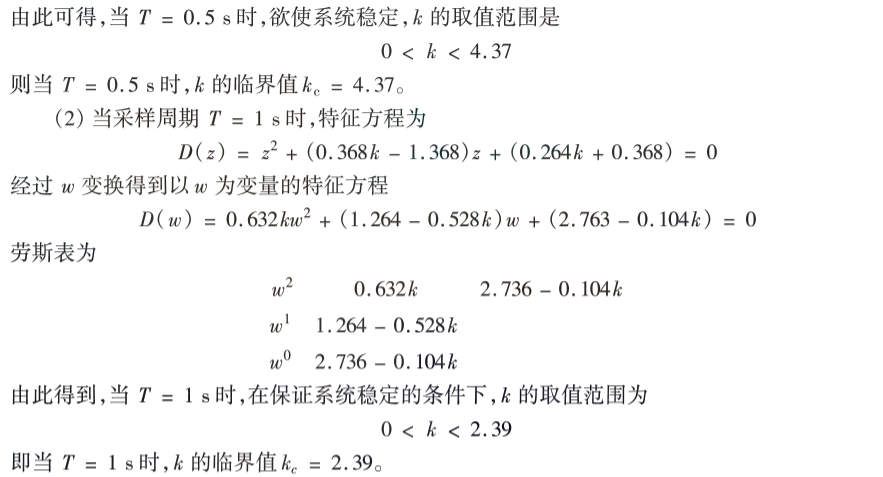
\includegraphics[width = .8\textwidth]{note/system stability/figure/15.png}
    \end{center}
\end{example}

\subsection{线性离散系统的稳态误差}

\subsubsection{稳态误差与稳态误差终值}

和连续系统类似，离散系统的误差信号的脉冲序列$e^* (t)$反映了在采样时刻系统希望输出与实际输出之差，当$t \geq t_s$，即过渡过程结束后，系统误差信号的脉冲序列就是离散系统的稳态误差。一般记为
\begin{equation*}
    e^*_{ss}(t) \quad t\geq t_s
\end{equation*}
同样的，当$t \to \infty$时，可以求得线性离散系统在采样点上的稳态误差终值：
\begin{equation*}
    e^*_{ss}(\infty) = \lim_{t\to \infty} e^* (t) = \lim _{t \to \infty} e^*_{ss}(t)
\end{equation*}
如果误差信号的Z变换为$E(z)$，在满足Z变换终值定理使用条件的情况下，可以利用Z变换的中值定理求离散系统稳态误差的终值
\begin{equation*}
    e^*_{ss}(\infty) = \lim_{t\to \infty} e^* (t) = \lim_{z\to 1}(z-1)E(z)
\end{equation*}

\subsubsection{稳态误差系数}
和连续系统类似，线性离散系统也存在几个静态误差系数，具体为：
\begin{enumerate}
    \item 静态位置误差系数：$K_p = \lim\limits_{z\to 1} GH(z)$
    \item 静态速度误差系数：$K_v = \lim\limits_{z\to 1} (z-1)GH(z)$
    \item 静态加速度误差系数：$K_a = \lim\limits_{z\to 1} (z-1)^2 GH(z)$
\end{enumerate}

\begin{center}
    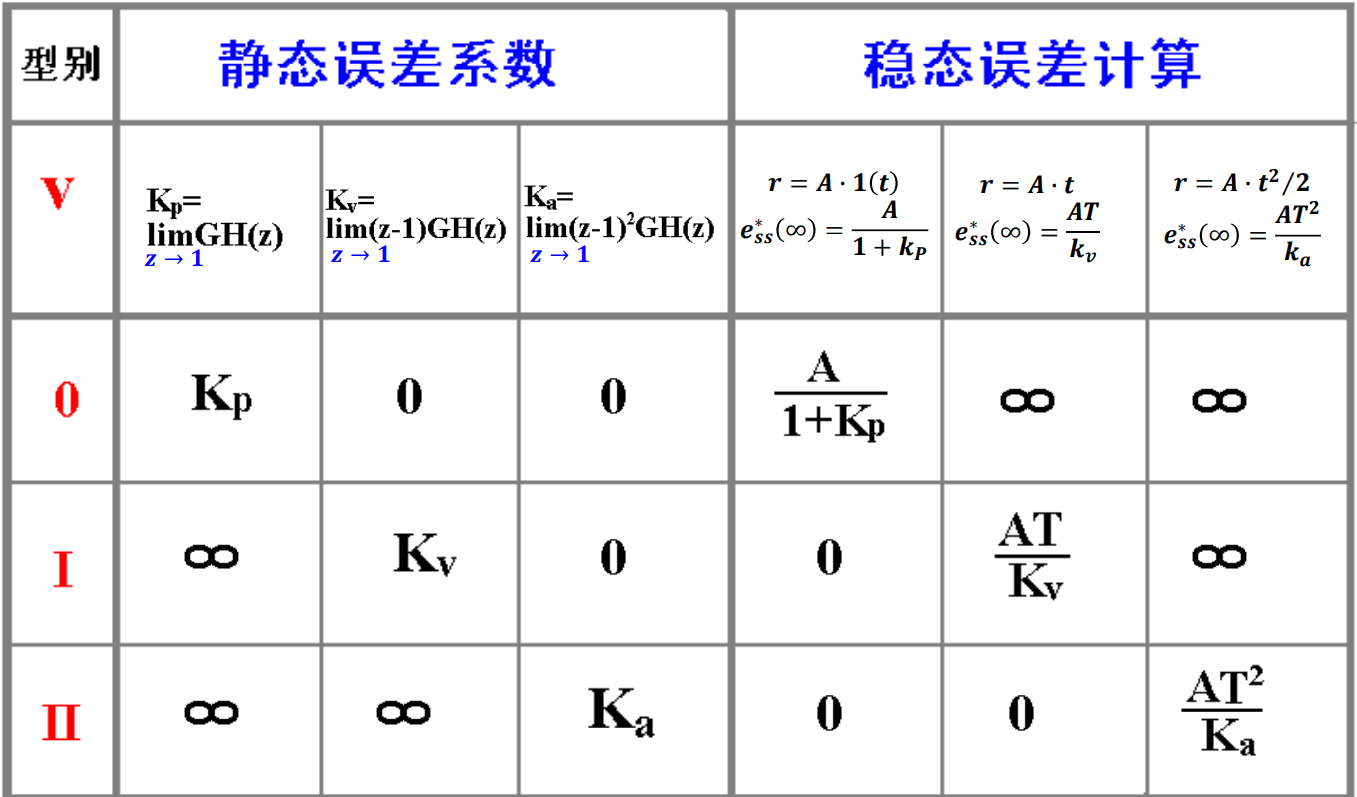
\includegraphics[width = .6\textwidth]{note/system stability/figure/16.png}
\end{center}

\subsubsection{动态误差系数}

与连续系统类似，我们也可以定义离散系统的动态误差系数

若系统闭环误差传递函数为$\Phi_e(z)$，根据Z变换的定义，将$z = e^{sT}$代入$\Phi_e(z)$，可以得到以$s$为变量的闭环误差脉冲传递函数：
\begin{equation*}
    \Phi_e^* (s) = \Phi_e^* (z) \left|_{z = e^{sT}}  \right.
\end{equation*}

\begin{center}
    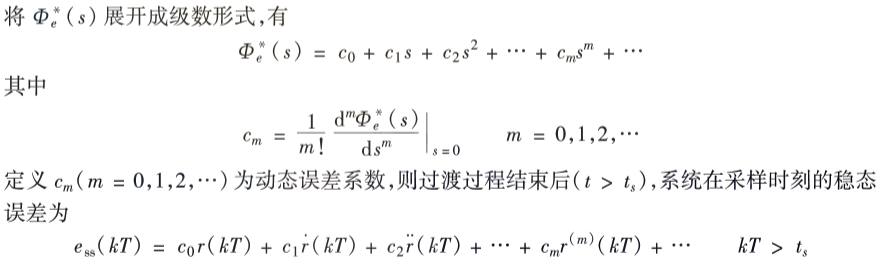
\includegraphics[width = .9\textwidth]{note/system stability/figure/17.png}
\end{center}

\partsimage{cov18.pdf}
\part{控制系统的设计与综合}

\chapterimage{13.jpg}
\chapter{控制系统的性能指标}
\label{chap:performance-metrics}

\section{稳定裕度}

关于稳定裕度的部分，详情请见系统稳定性与分析中的\hyperref[sec:stability-margin]{稳定裕度}这一节，本章不再复述其定义，只谈其应用。

以下部分均以二阶系统为例进行讨论：

\subsection{二阶系统的稳定裕度}

在经典二阶单位反馈系统（如下图）中，我们可以写出其开环传递函数为：
\begin{center}
    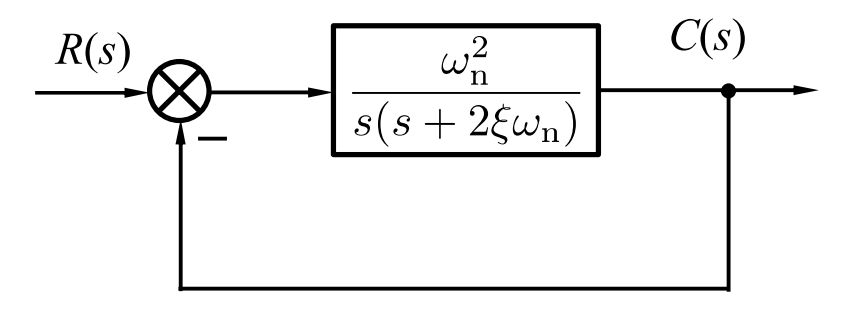
\includegraphics[width=.5\textwidth]{note/performance metrics/figure/1.png}
\end{center}
\begin{equation*}
    G(s) = \frac{\omega_n^2}{s^2 + 2 \omega_n \xi s}
\end{equation*}

故由剪切频率的定义可知：$\omega_c = \omega_n \sqrt{{\sqrt{4 \xi^4 + 1} - 2\xi^2}}$

其相角裕度为：$\gamma = 90\text{°} - \arctan{\dfrac{\sqrt{\sqrt{4 \xi^4 + 1} - 2\xi^2}}{2 \xi}}$

由于其穿越频率$\omega_g = \infty$，故其相位裕度$K_g = \infty$

\section{闭环频域的性能指标}
对于一个一般的系统，我们可以给出其广义的示意图如下：
\begin{center}
    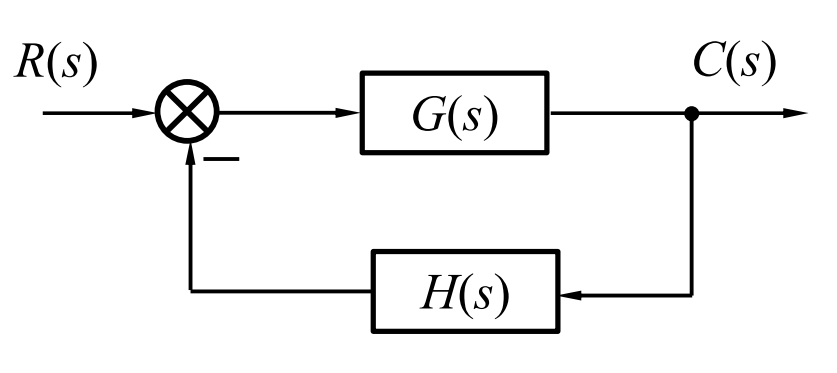
\includegraphics[width=.5\textwidth]{note/performance metrics/figure/2.png}
\end{center}

根据上图，我们可以给出其前向通路和反馈通路的表达式如下：
\begin{enumerate}
    \item 前向通路：$G(s) = \dfrac{K G_1(s)}{s^v}$
    \item 反馈通路：$H(s) = K_h H_1(s)$
\end{enumerate}

其中$K$为前向通路增益，$K_h$为反馈通路的增益，$G_1(s)$和$H_1(s)$在0处均有值为1。

所以闭环传递函数的频域幅值为：
\begin{equation*}
    \begin{split}
        A(\omega) &= \left\lvert \frac{G(j\omega)}{1 + G(j\omega) H(j\omega)} \right\rvert     \\
        &=\frac{\left\lvert K G_1(j\omega)\right\rvert}{\left\lvert (j\omega)^v + K K_h G_1(j\omega) H_1(j\omega)\right\rvert }
    \end{split}
\end{equation*}

根据上面的式子我们可以得到幅值在0处的值为：
\begin{equation*}
    A(0) = 
    \begin{cases}
        \frac{1}{K_h} & v\geq 1 \\
        \frac{K}{1 + K K_h} & v = 0\\ 
    \end{cases}
\end{equation*}

故$1-A(0)$为单位阶跃响应的稳态误差



\textbf{闭环频域的性能指标一共有以下几个：}
\begin{enumerate}
    \item 零频幅值：即$A(0)$
    \item 相对谐振峰值：$M_r = \dfrac{\max A(\omega)}{A(0)}$
    \item 谐振频率：出现谐振峰值时的频率，其满足$A(\omega_r) = \max_{\omega} A(\omega)$
    \item 截止频率：幅值下降到零频幅值的$\frac{\sqrt{2}}{2}$时的频率，即 $A(\omega_b) = \frac{\sqrt{2}}{2} A(0)$
\end{enumerate}

\subsection{二阶系统的闭环频域性能}
对于一个经典二阶系统（如下图所示）我们可以给出其闭环频率特性和幅频特性：
\begin{center}
    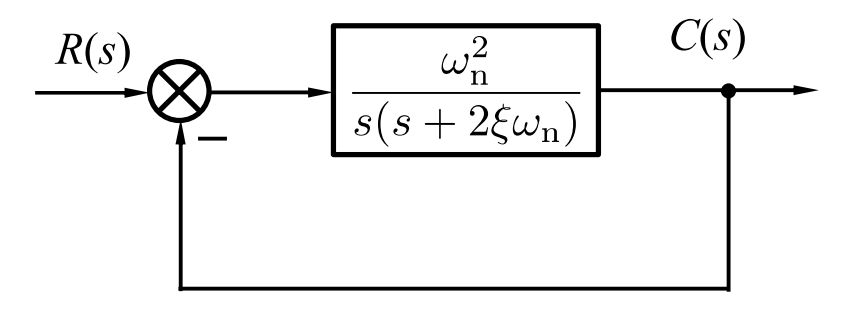
\includegraphics[width = .5\textwidth]{note/performance metrics/figure/1.png}
\end{center}
\begin{equation*}
    \begin{split}
        \Phi(j \omega) &= \frac{\omega_n^2}{(j\omega)^2 + 2j\xi \omega_n \omega + \omega_n^2} \\
        A(\omega) &= \left\lvert \Phi(j\omega) \right\rvert = \frac{\omega_n^2}{\sqrt{(\omega_n^2 - \omega^2)^2 + 4 \xi^2 \omega_n^2 \omega^2}}\\
    \end{split}
\end{equation*}

同时我们可以给出闭环幅频特性曲线如下：
\begin{center}
    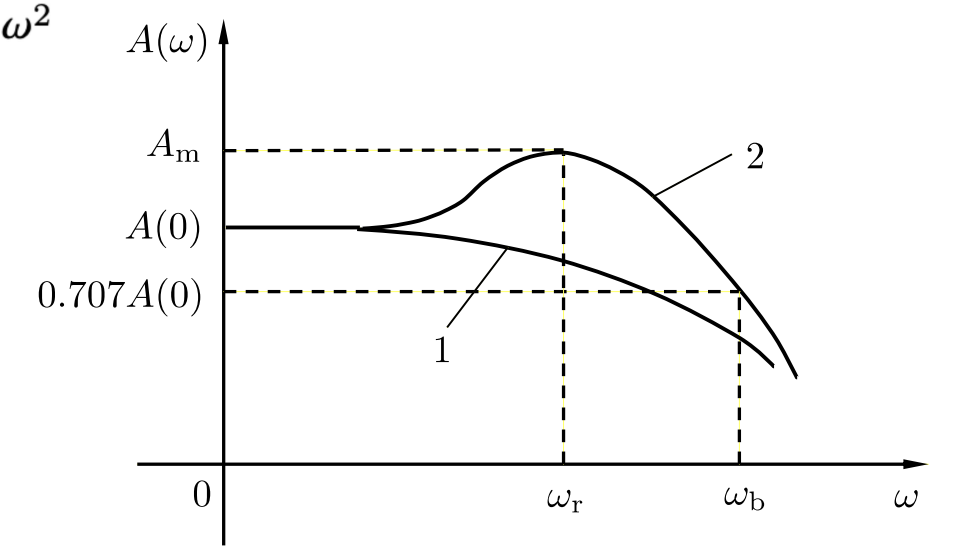
\includegraphics[width = .5\textwidth]{note/performance metrics/figure/3.png}
\end{center}

由图和式子可以知道谐振频率$\omega_r = \omega_n \sqrt{1-2 \xi^2}$，相对谐振峰值$M_r = \frac{1}{2 \xi \sqrt{1-\xi^2}}$

同样的，根据截止频率的定义我们也可以得到谐振频率的式子为：$\omega_b = \omega_n \sqrt{1-2\xi^2 + \sqrt{2 - 4\xi^2 + 4\xi^4}}$

\subsection{闭环特性的图示法：等M圆}
设系统为单位负反馈系统，设开环传递函数$G(j \omega) = U + jV$，闭环传递函数的幅值为$M$，则有：
\begin{equation*}
    (U + \frac{M^2}{M^2 - 1})^2 + V^2 = \frac{M^2}{(M^2 - 1)^2}
\end{equation*}

由式子可知，这是一个关于开环传递函数实部和虚部的一个圆，圆的圆心和半径由闭环频率特性的幅值确定，等M圆示意图如下：
\begin{center}
    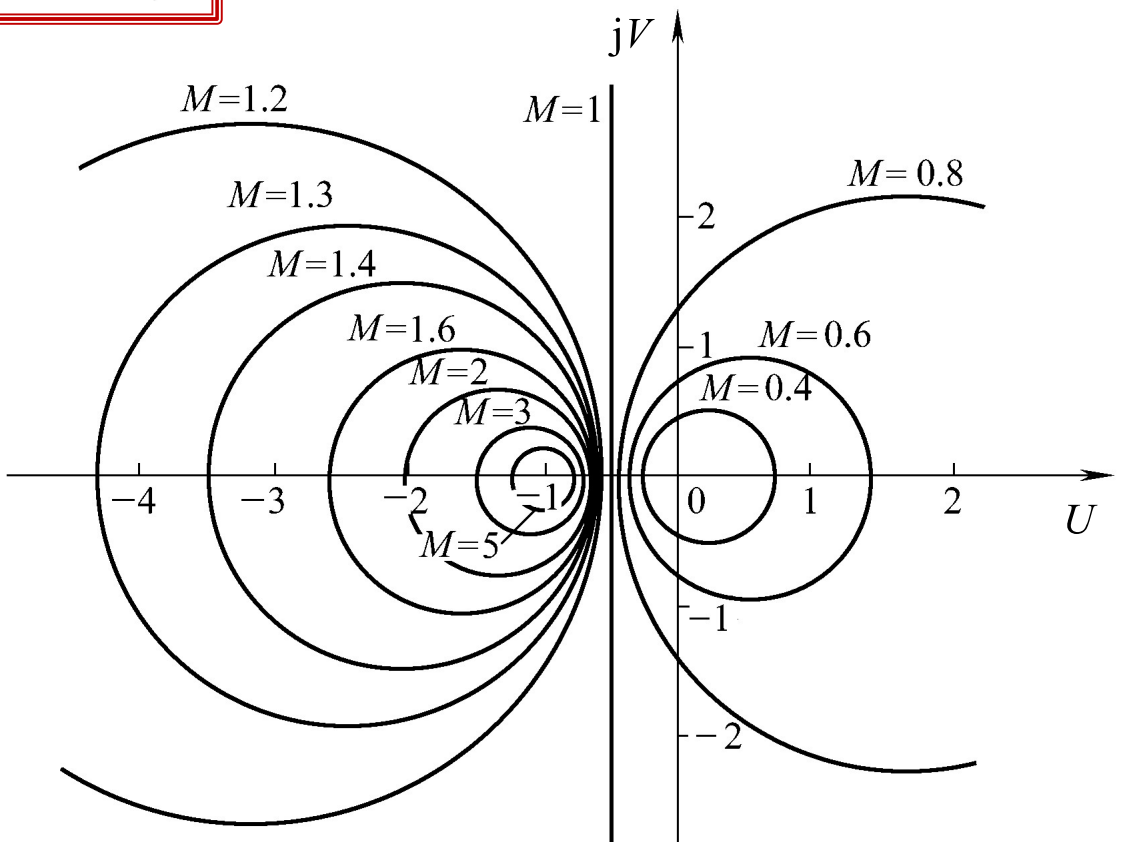
\includegraphics[width = .5\textwidth]{note/performance metrics/figure/4.png}
\end{center}

由图和式子我们可以得到：
\begin{enumerate}
    \item $M > 1$时，圆心在虚轴左侧，且半径随$M$的增大而减小，当$M \to \infty$时圆心在(-1,0)处
    \item $M < 1$时，圆心在虚轴的右侧，且半径随$M$的增大而增大，当$M \to 0$时圆心在(0,0)处
    \item $M = 1$时，圆退化为直线$U = -\frac{1}{2}$
\end{enumerate}

等M圆的具体用法如下：

我们可以在等M圆图里画出系统的Nyquist曲线，根据曲线和等M圆的相交的情况可以确定系统的闭环幅频特性曲线，当Nyquist曲线与某一M圆相切时，相切M圆的M值就是闭环幅频特性的谐振峰值$M_r$，切点处的$\omega$就是谐振频率$\omega_r$

\section{不同域下性能指标的关系}

\subsection{闭环频域指标和开环频域指标之间的关系}

对于单位反馈系统，如果$G(s)$是I型或以上系统，则有$A(0) = 1$；如果$G(s)$是0型系统，且其开环增益较高，则有$A(0) \approx 1$。则有以下式子成立：
\begin{equation*}
    M_r = \frac{A_{max}}{A(0)} \approx \frac{1}{\sin \gamma}
\end{equation*}
或者
\begin{equation*}
    \gamma = \arcsin \frac{1}{M_r}
\end{equation*}
根据以上两个式子，以及7.1.1中的$w_c$和$\gamma$，和7.2.1中的$M_r$，$\omega_r$，$\omega_b$我们可以得到经典二阶系统中的闭环频域指标和开环频域指标的关系为：
\begin{center}
    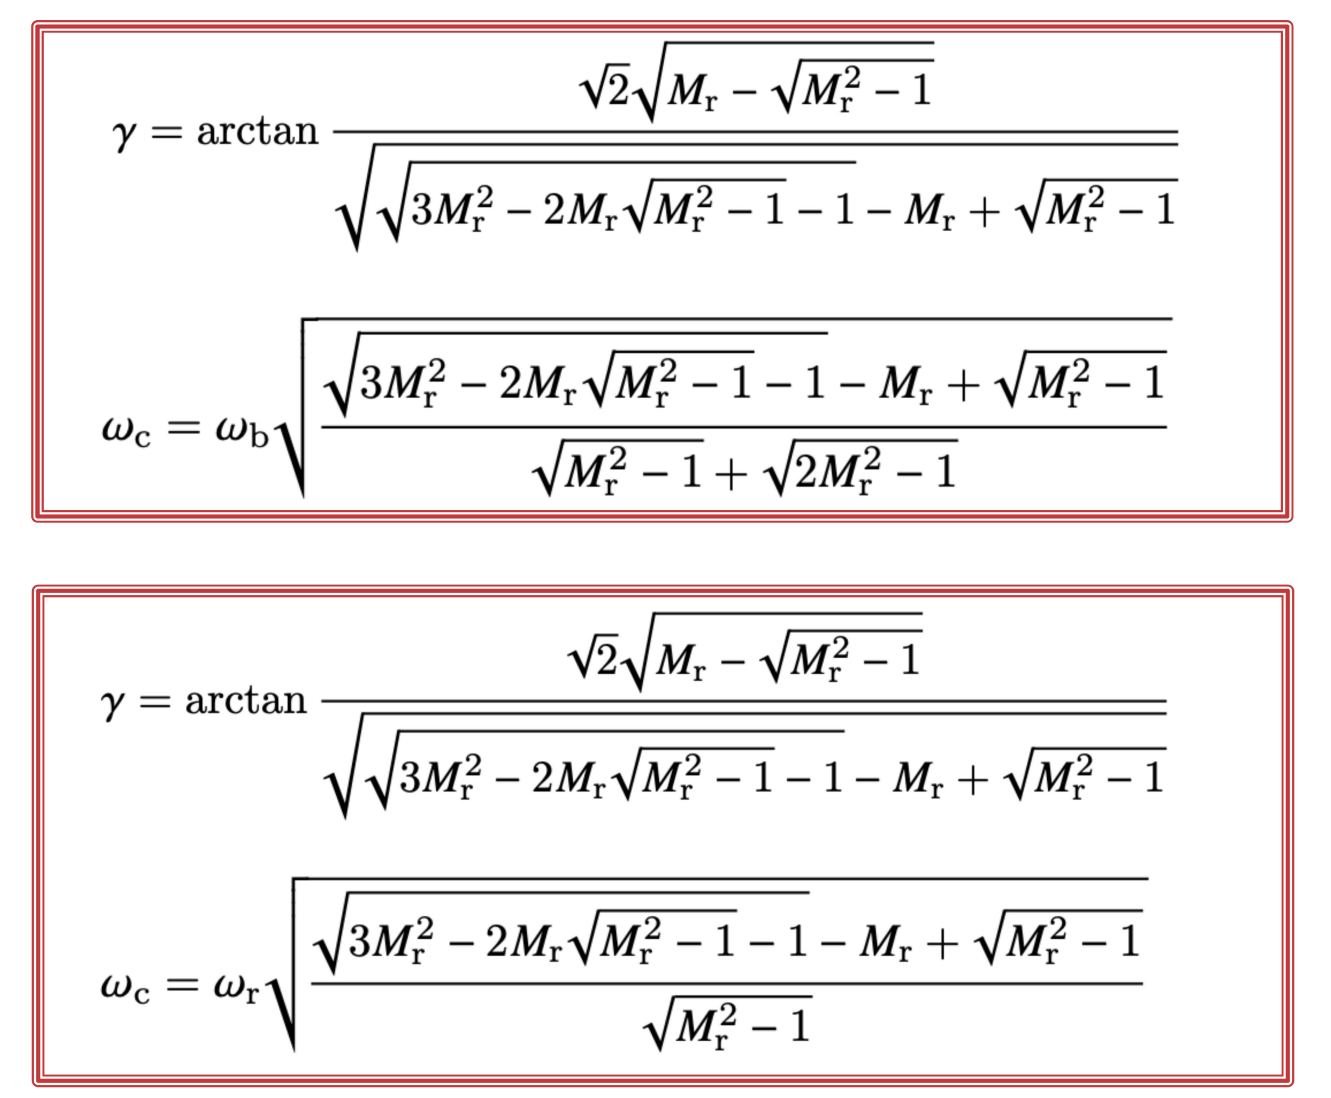
\includegraphics[width = .7\textwidth]{note/performance metrics/figure/5.png}
\end{center}

\subsection{闭环频域指标和时域指标之间的关系}

在经典二阶系统时域中，我们有以下几个指标：
\begin{enumerate}
    \item $\sigma_p = \text{exp}\left( \frac{-\xi \pi}{\sqrt{1- \xi^2 }}\right)$
    \item $t_s = \frac{4}{\xi \omega_n} \quad \Delta = 0.05$
    \item $t_p = \frac{\pi}{\omega_n \sqrt{1 - \xi^2}}$
\end{enumerate}

再根据7.1.1中的$w_c$和$\gamma$，和7.2.1中的$M_r$，$\omega_r$，$\omega_b$我们可以得到经典二阶系统中的闭环频域指标和时域指标的关系为：

\begin{center}
    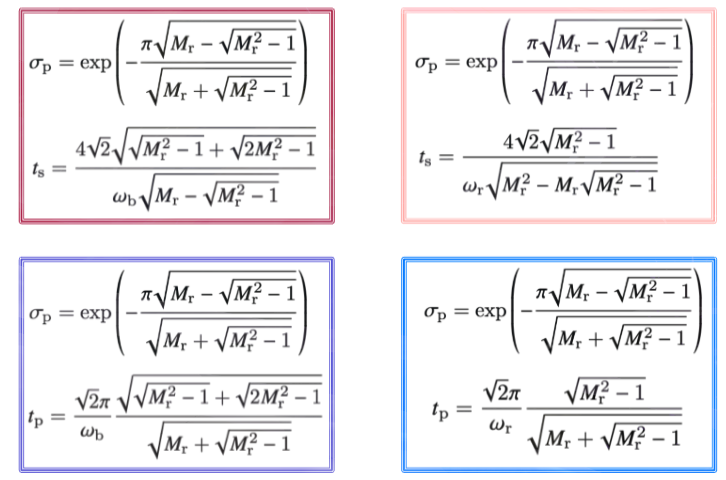
\includegraphics[width = .6\textwidth]{note/performance metrics/figure/6.png}
\end{center}

由于这上面几组式子太难算了，前人在此基础上得到了经验公式：

\begin{center}
    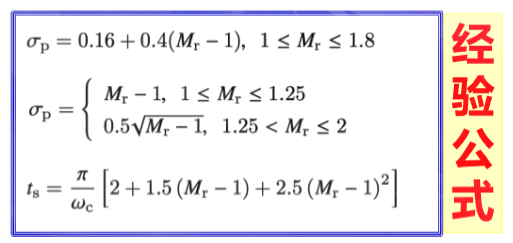
\includegraphics[width = .6\textwidth]{note/performance metrics/figure/7.png}
\end{center}

\subsection{开环频域指标和时域指标之间的关系}

由上面的式子可以知道有以下几组式子成立：
\begin{equation*}
    \begin{split}
        \sigma_p &= \text{exp}\left( \frac{-\pi}{\sqrt{2 \sqrt{M^2 - 1} - 1}} \right) \\
        M &= \frac{2 + \tan^2 \gamma}{\tan^2 \gamma} \\
        \omega_c t_p &= \frac{2\pi}{\tan \gamma} \frac{1}{\sqrt{ 2 \sqrt{M^2 - 1} - 1}}\\
        t_s &= \frac{8}{\omega_c \tan \gamma}
    \end{split}
\end{equation*}

同样的，在这组式子的基础上前人也总结出了一组经验公式：
\begin{center}
    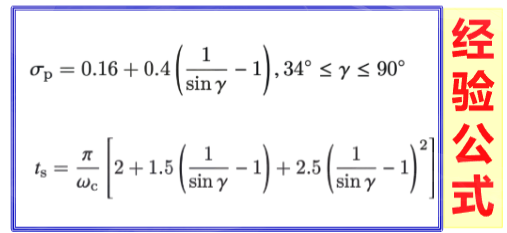
\includegraphics[width = .6\textwidth]{note/performance metrics/figure/8.png}
\end{center}

\section{三频段理论}

\subsection{三频段的划分}
根据Bode中的频率与剪切频率，转折频率等特殊频率之间的关系我们可以将Bode图划分为以下图中的三段：
\begin{center}
    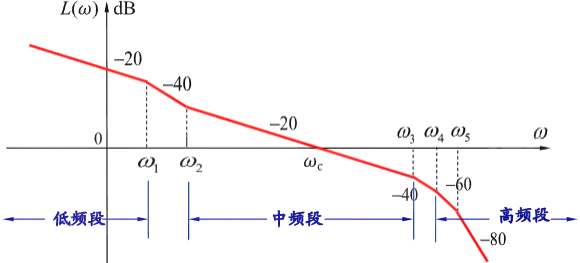
\includegraphics[width = .5\textwidth]{note/performance metrics/figure/9.png}
\end{center}
\begin{enumerate}
    \item 低频段：第一个转折频率之前的频段
    \item 中频段：剪切频率附近的频段，一般为剪切频率前一个转折频率到剪切频率后一个转折频率之间的频段
    \item 高频段：通常为中频段之后的频段，一般为$\omega > 10 \omega_c$的频段，其中$\omega_c$为剪切频率，这部分特性是由系统中小时间常数的环节决定的，由于远离剪切频率，一般分贝值又比较低，故对系统的动态响应影响不大

    在高频段，由于系统的开环幅频特性$G(j\omega)$远小于1，因此对单位负担亏系统有：
    \begin{equation*}
        \left\lvert \Phi(j\omega) \right\rvert = \left\lvert \frac{G(j\omega)}{1 + G(j\omega)} \right\rvert \approx \left\lvert G(j\omega) \right\rvert 
    \end{equation*}
    故在高频段，开环与闭环对数幅频特性近似相等，直接反映了系统抑制输入端高频干扰的能力。高频段的分贝值越低，系统的抗干扰能力就越强
\end{enumerate}

\subsection{两类特殊的中频段}
下面我们将讨论中频段斜率分别为-20dB/dec和-40dB/sec时的特性
\begin{enumerate}
    \item 中频段斜率为-20dB/sec时：\\
          此时这一段的开环传递函数和闭环传递函数可以近似为：
          \begin{equation*}
            \begin{split}
                G(s) &= \frac{K}{s} \\
                \Phi(s) &= \frac{K}{s + K} = \frac{1}{\frac{s}{K} + 1}               
            \end{split}
          \end{equation*}
          此时系统非常容易稳定
    \item 中频段斜率为-40dB/sec时：\\
          此时这一段的开环传递函数和闭环传递函数可以近似为：
          \begin{equation*}
            \begin{split}
                G(s) &= \frac{K}{s^2} \\
                \Phi(s) &= \frac{K}{s^2 + K} = \frac{\omega_c^2}{s^2 + \omega_c^2}
            \end{split}
          \end{equation*}
\end{enumerate}

\subsection{一个设计合理的系统的三频段的要求}
对于一个设计合理的系统的三频段，我们有以下的要求:
\begin{enumerate}
    \item 中频段的斜率以-20dB/sec为宜
    \item 低频段和高频段可以有更大的斜率，低频段的斜率越大，系统的稳态性能越强，高频段的斜率越大，系统排除干扰的能力越强
    \item 中频段必须有足够的带宽，以保证系统的相位裕量，带宽越大，相位裕量越大；$\omega_c$的大小也很重要，$\omega_c$越大系统的快速性越好，但是抗干扰的能力会下降
\end{enumerate}

\subsection{低频段和高频段的斜率对中频段剪切频率的影响}

\subsubsection{低频段对中频段剪切频率的影响}

\begin{center}
    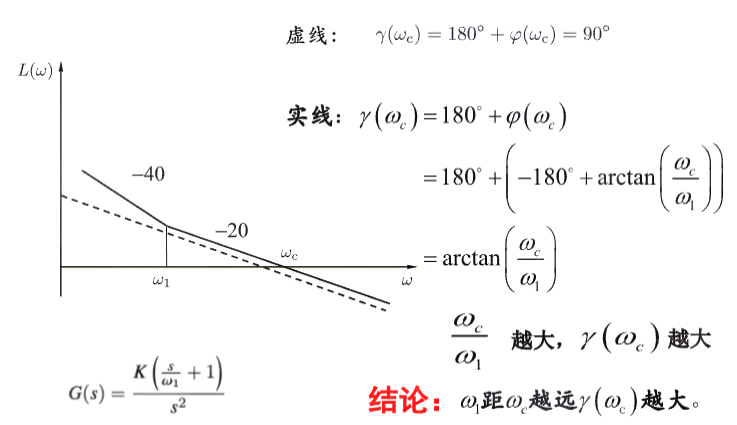
\includegraphics[width = .8\textwidth]{note/performance metrics/figure/10.png}
\end{center}

\subsubsection{高频段对中频段剪切频率的影响}

\begin{center}
    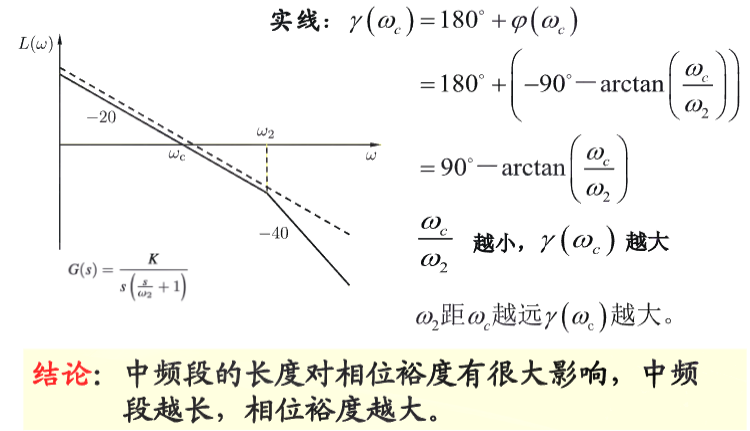
\includegraphics[width = .8\textwidth]{note/performance metrics/figure/11.png}
\end{center}

\subsection{开环增益变化对相位裕度的影响}

\begin{center}
    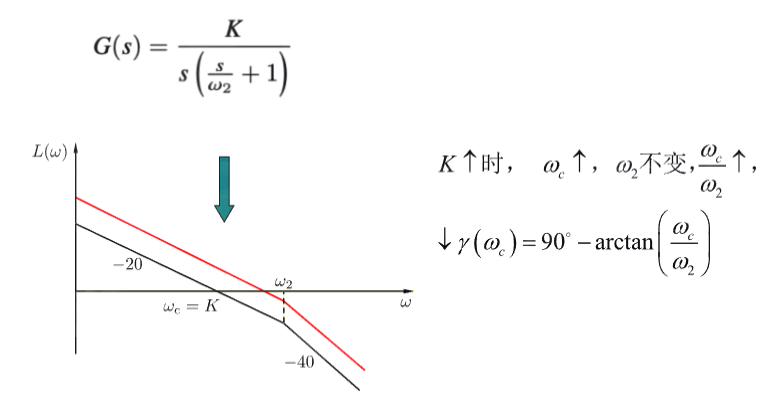
\includegraphics[width = .8\textwidth]{note/performance metrics/figure/12.png}

    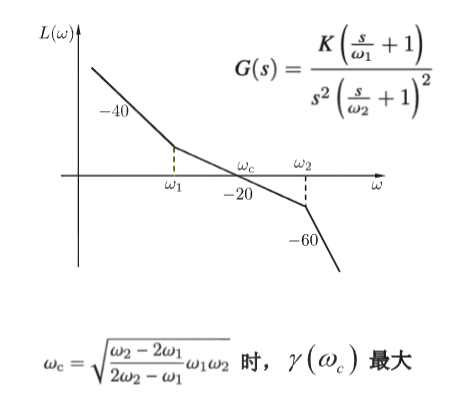
\includegraphics[width = .4\textwidth]{note/performance metrics/figure/13.png}

    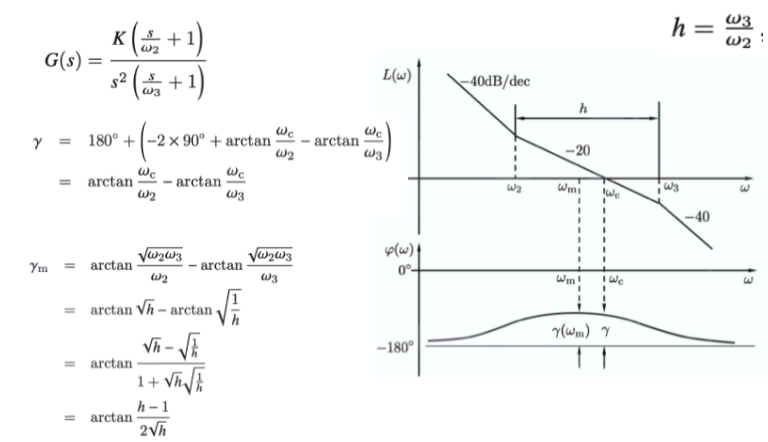
\includegraphics[width = .6\textwidth]{note/performance metrics/figure/14.png}
\end{center}


\chapterimage{14.jpg}
\chapter{基于频率特性的校正}
\section{串联超前校正}

\subsection{超前环节的性质}
超前校正环节具有如下的性质：
\begin{enumerate}
    \item 传递函数：$G_c(s) = \frac{\tau s + 1}{T s + 1} \quad \tau > T$
    \item 频率特性：$G_c(j\omega) = \frac{j\tau \omega + 1}{jT\omega + 1}$
    \item 相频特性：$\varphi (\omega) = \angle G_c(j\omega) = \arctan \tau \omega - \arctan T \omega$
    \item 幅频特性：$\left\lvert G_c(j\omega) \right\rvert = \frac{\sqrt{\tau^2 \omega^2 + 1}}{\sqrt{T^2 \omega^2 + 1}} $
    \item 最大相角对应的频率在转折频率的中点，即：$\omega_m = \frac{1}{\sqrt{T\tau}}$，此时相角：$\varphi_m = \arctan \frac{\tau - T}{2\sqrt{T \tau}}$\\
    若假设$\tau = \alpha T$，则有：$\omega_m = \frac{1}{T\sqrt{\alpha}}, \quad  \varphi_m = \arctan \frac{\alpha - 1}{2\sqrt{\alpha}} = \arcsin \frac{\alpha - 1}{\alpha + 1} $，当相角取最大时对应的幅频特性：$L_c(\omega_m) = 20 \lg \frac{\tau}{T \sqrt{\alpha}} = 10\lg \alpha$，示意图如下：

    \begin{center}
        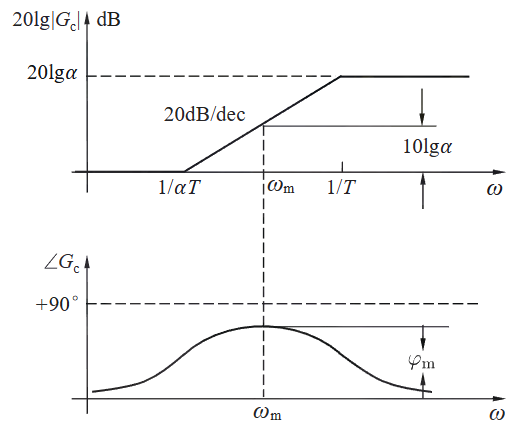
\includegraphics[width = .4\textwidth]{note/frequency correction/figure/1.png}
    \end{center}
\end{enumerate}

\subsection{单级超前校正的设计流程}

\subsubsection{相角裕度优先超前校正设计}
我们通过以下的步骤，以相角裕度要求优先为原则设计：
\begin{enumerate}
    \item 根据所要求的稳态性能指标确定系统的开环增益
    \item 利用已知的开环增益，绘制原系统的Bode图，并计算未校正系统的剪切频率$\omega_{c0}$，相角裕度$\gamma_0$
    \item 根据相角裕度的要求确定超前校正环节的$\alpha$，为使相角裕度达到要求值，计算所需增加的超前相角$\varphi_m$，即
    \begin{equation*}
        \varphi_m = \gamma - \gamma_0 + \Delta
    \end{equation*}
    上式中$\gamma$为要求的相角裕度，$\Delta$是因为考虑到校正装置影响剪切频率的位置而附加的相角，一般取$\Delta = 5\text{°} \sim  10 \text{°}$，然后根据下面这个式子计算出$\alpha$：
    \begin{equation*}
        \alpha = \frac{1+\sin \varphi_m}{1-\sin \varphi_m}
    \end{equation*}
    \item 确定校正后的系统的剪切频率$\omega_c$，在校正后的剪切频率处，未校正系统的负幅值由超前校正环节补偿，因此校正后系统的剪切频率$\omega_c$由以下的式子确定：
    \begin{equation*}
        20 \lg \left\lvert G_0(\omega_c) \right\rvert = -10 \lg \alpha
    \end{equation*}
    如果此时求得的剪切频率满足设计要求，则进行下一步；否则返回第三步调整$\Delta$
    \item 确定超前校正环节，让超前矫正环节取得最大值的频率对准校正后系统的剪切频率，即$\omega_m = \omega_c$，根据以下的式子：
    \begin{equation*}
        T = \frac{1}{\omega_m \sqrt{\alpha}}
    \end{equation*}
    确定校正装置的实践常数，进而确定校正环节的传递函数
    \item 检验系统的性能指标，若不满足要求，回到第三步重新取$\Delta$
\end{enumerate}

\subsubsection{剪切频率优先超前校正设计流程}
我们通过以下的步骤，以剪切频率要求优先为原则设计：
\begin{enumerate}
    \item 根据所要求的稳态性能指标确定系统的开环增益
    \item 利用已知的开环增益，绘制原系统的Bode图，并计算未校正系统的剪切频率$\omega_{c0}$，相角裕度$\gamma_0$
    \item 根据设计要求确定校正后系统的剪切频率$\omega_c$，并让超前校正环节取最大相角的频率对准该剪切频率，即$\omega_m = \omega_c$
    \item 根据幅值补偿确定超前校正环节的$\alpha$，在校正后的剪切频率处，未校正系统的负幅值由超前校正环节补偿，因此校正后系统的剪切频率$\omega_c$由以下的式子确定：
    \begin{equation*}
        20 \lg \left\lvert G_0(\omega_c) \right\rvert = -10 \lg \alpha
    \end{equation*}
    根据上式确定$\alpha$，按照下面的式子计算$\varphi_m$：
    \begin{equation*}
        \varphi_m = \arcsin \frac{\alpha - 1}{\alpha + 1} 
    \end{equation*}
    如果$\varphi_m = \gamma - \gamma_0 + \Delta$，$\Delta = 5\text{°} \sim  10 \text{°}$，则进行下一步，否则，返回第三步重新选择剪切频率
    \item 确定超前校正环节，由第三步和第四步确定的$\omega_m$和$\alpha$，根据以下的式子：
    \begin{equation*}
        T = \frac{1}{\omega_m \sqrt{\alpha}}
    \end{equation*}
    确定校正装置的实践常数，进而确定校正环节的传递函数
    \item 检验系统的性能指标，若不满足要求，回到第三步重新取剪切频率
\end{enumerate}

\subsubsection{相角裕度优先超前校正修正设计}
传统的相角裕度优先设计可能取不到特别合适的$\varphi_m$，所以我们通过以下的步骤，修正上述的流程
\begin{enumerate}
    \item 根据所要求的稳态性能指标确定系统的开环增益
    \item 利用已知的开环增益，绘制原系统的Bode图，并计算未校正系统的剪切频率$\omega_{c0}$，相角裕度$\gamma_0$
    \item 根据相角裕度的要求确定超前校正环节的$\alpha$，为使相角裕度达到要求值，计算所需增加的超前相角$\varphi_m$，即
    \begin{equation*}
        \varphi_m = \gamma - \gamma_0(\omega_{cL})
    \end{equation*}
    上式中$\gamma$为要求的相角裕度，$\gamma_0(\omega)$为未校正系统在$\omega$处的相位储备，$\omega_{cL}$为所要求的剪切频率的下界，根据$\varphi_m$和$\alpha$之间的关系计算出$\alpha$
    \item 确定校正后的系统的剪切频率$\omega_c$，在校正后的剪切频率处，未校正系统的负幅值由超前校正环节补偿，因此校正后系统的剪切频率$\omega_c$由以下的式子确定：
    \begin{equation*}
        20 \lg \left\lvert G_0(\omega_c) \right\rvert = -10 \lg \alpha
    \end{equation*}
    如果此时求得的剪切频率满足设计要求，则进行下一步；否则返回第三步调整$\varphi_m$
    \item 确定超前校正环节，让超前矫正环节取得最大值的频率对准校正后系统的剪切频率，即$\omega_m = \omega_c$，根据以下的式子：
    \begin{equation*}
        T = \frac{1}{\omega_m \sqrt{\alpha}}
    \end{equation*}
    确定校正装置的实践常数，进而确定校正环节的传递函数
    \item 检验系统的性能指标，若不满足要求，回到第三步重新取$\varphi_m$
\end{enumerate}

\subsection{多级超前校正设计流程}
多级超前校正设计流程可以转化为多个单级超前校正设计，后一级的超前校正以前一级超前校正的结果为条件，最后计算出的结果满足条件即可。

\textbf{注意：}如果出现$\omega_r$和$M_r$为题设要求的题要将题设条件转化为$\gamma$和$\omega_c$的条件，其中$\omega_c$的计算就是将系统强行等效为一个二阶系统，利用二阶系统的$\omega_c$与$\omega_r$之间的关系进行求解

\section{串联迟后校正}

\subsection{迟后校正环节的性质}
迟后校正环节具有如下性质：
\begin{enumerate}
    \item 传递函数：$G_c(s) = \frac{\tau s + 1}{\beta \tau s + 1}, \quad \beta > 1$
    \item 频率特性：$G_c(j\omega) = \frac{j\tau \omega + 1}{j \beta \tau \omega + 1},\quad \beta > 1$
    \item 相频特性：$\varphi(\omega) = \angle G_c(j\omega) = \arctan \tau \omega - \arctan \beta \tau \omega$
    \item 幅频特性：$\left\lvert G_c(j\omega) \right\rvert = \frac{\sqrt{\tau^2 \omega^2 + 1}}{\sqrt{\beta^2 \tau^2 \omega^2 + 1}} $
    \item 迟后校正环节的最小相角对应的频率在转折频率的中点，即：$\omega_m = \frac{1}{\tau\sqrt{\beta}}$，且有：$\varphi_m = \arctan \frac{1 - \beta}{2\sqrt{\beta}}$，具体示意图如下：
    \begin{center}
        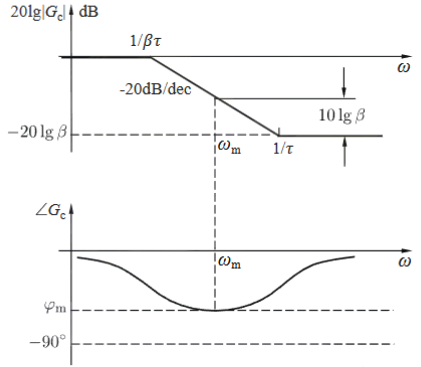
\includegraphics[width = .4\textwidth]{note/frequency correction/figure/2.png}
    \end{center}
\end{enumerate}

\subsection{单级串联迟后校正环节设计流程}

\subsubsection{相位裕度优先迟后校正设计}
我们通过以下的步骤，以相角裕度要求优先为原则设计：
\begin{enumerate}
    \item 按稳态性能的要求确定系统的型别和开环增益
    \item 利用已知的开环增益，绘制未校正系统$G_0(j\omega)$的Bode图，并计算未校正系统的剪切频率$\omega_{c0}$和相角裕度$\gamma_0$
    \item 确认校正后系统的剪切频率$\omega_c$，该剪切频率应该满足下式：
    \begin{equation*}
        180\text{°}+ \angle G_0(j\omega_c) = \gamma + \Delta
    \end{equation*}
    其中$\gamma$为要求的相角裕度，$\Delta$是由于校正装置产生的相位迟后效应而附加的相角
    \item 确定校正装置的$\beta$值，为使校正后的系统在剪切频率出幅频特性为0dB，应有：
    \begin{equation*}
        20 \lg \left\lvert G_0(j\omega_c) \right\rvert - 20\lg \beta = 0 
    \end{equation*}
    即
    \begin{equation*}
        \beta = \left\lvert G_0(j\omega_c) \right\rvert 
    \end{equation*}
    \item 确定迟后校正环节的参数$\tau$，为减小串联迟后校正对系统相位裕度的影响，要求矫正环节在剪切频率$\omega_c$处的迟后相移在6°$\sim$12°以下，应当选择：
    \begin{equation*}
        \tau = (5 \sim 10) \frac{1}{\omega_c}
    \end{equation*}
    \item 校验校正后系统的相位裕度和其余性能指标，如不满足要求，返回第三步重新选择$\Delta$，直到满足要求
\end{enumerate}

\subsubsection{剪切频率优先迟后校正设计}
我们通过以下的步骤，以剪切频率要求优先为原则设计：
\begin{enumerate}
    \item 按稳态性能的要求确定系统的型别和开环增益
    \item 利用已知的开环增益，绘制未校正系统$G_0(j\omega)$的Bode图，并计算未校正系统的剪切频率$\omega_{c0}$和相角裕度$\gamma_0$
    \item 确认校正后系统的剪切频率$\omega_c$，该剪切频率应该满足下式：
    \begin{equation*}
        180\text{°}+ \angle G_0(j\omega_c) > \gamma + \Delta
    \end{equation*}
    其中$\gamma$为要求的相角裕度，$\Delta$是由于校正装置产生的相位迟后效应而附加的相角
    \item 确定校正装置的$\beta$值，为使校正后的系统在剪切频率出幅频特性为0dB，应有：
    \begin{equation*}
        20 \lg \left\lvert G_0(j\omega_c) \right\rvert - 20\lg \beta = 0 
    \end{equation*}
    即
    \begin{equation*}
        \beta = \left\lvert G_0(j\omega_c) \right\rvert 
    \end{equation*}
    \item 确定迟后校正环节的参数$\tau$，为减小串联迟后校正对系统相位裕度的影响，要求矫正环节在剪切频率$\omega_c$处的迟后相移在6°$\sim$12°以下，应当选择：
    \begin{equation*}
        \tau = (5 \sim 10) \frac{1}{\omega_c}
    \end{equation*}
    \item 校验校正后系统的相位裕度和其余性能指标，如不满足要求，返回第三步重新选择$\Delta$，直到满足要求
\end{enumerate}

\section{串联迟后-超前校正}
在此设计方法中，迟后校正的主要作用使降低系统的剪切频率，不关注它对系统相角裕度的影响；相角裕度提高的任务交给超前校正环节

尽管如此，由于迟后校正环节降低了剪切频率，通过利用原系统的相位储备，迟后校正后系统的相角裕度事实上得到了部分提升

\subsection{迟后环节优先的迟后-超前校正环节设计}

\subsubsection{剪切频率优先设计流程}
我们通过以下的步骤，以剪切频率要求优先为原则设计：（针对超前校正而言）
\begin{enumerate}
    \item 绘制满足稳态误差要求的未校正系统开环频率特性的Bode图，由于串联超前校正可以有效增加相角裕度，所以首先\textbf{采用串联迟后校正，使系统的剪切频率满足或接近于满足设计要求}，在此基础上，再采用串联超前校正，使相角满足设计要求
    \item 考虑到进行串联超前校正时，会使原系统剪切频率增大，所以在进行串联迟后校正时可以使剪切频率略小于设计要求，使用剪切频率优先迟后校正发确定迟后校正环节
    \item 计算出串联迟后校正环节后的系统幅频特性曲线，求出剪切频率$\omega_c$和相角裕度$\gamma$
    \item 在这一步将对迟后校正后的系统进行超前校正，采用剪切频率优先超前校正法获得超前校正装置的传递函数
    \item 验证系统性能指标，如不满足要求，则回到第二步或者第四步重新设计
\end{enumerate}

\subsubsection{相角裕度优先设计流程}
我们通过以下的步骤，以剪切频率要求优先为原则设计：（针对超前校正而言）
\begin{enumerate}
    \item 绘制满足稳态误差要求的未校正系统开环频率特性的Bode图，由于串联超前校正可以有效增加相角裕度，所以首先\textbf{采用串联迟后校正，使系统的剪切频率满足或接近于满足设计要求}，在此基础上，再采用串联超前校正，使相角满足设计要求
    \item 考虑到进行串联超前校正时，会使原系统剪切频率增大，所以在进行串联迟后校正时可以使剪切频率略小于设计要求，使用剪切频率优先迟后校正发确定迟后校正环节
    \item 计算出串联迟后校正环节后的系统幅频特性曲线，求出剪切频率$\omega_c$和相角裕度$\gamma$
    \item 在这一步将对迟后校正后的系统进行超前校正，采用相角裕度优先超前校正法获得超前校正装置的传递函数
    \item 验证系统性能指标，如不满足要求，则回到第二步或者第四步重新设计
\end{enumerate}

\subsection{超前环节优先的迟后-超前校正环节设计}

\subsubsection{迟后环节提高稳态精度的超前环节优先的迟后-超前校正环节设计}

我们通过以下步骤进行校正环节的设计：（通过迟后环节提高稳态精度）
\begin{enumerate}
    \item 按稳态性能的要求确定系统的型别和开环增益$K$。利用已知的开环增益，绘制为校正系统$G_0(s)$的Bode图，并计算未校正系统的剪切频率$\omega_{c0}$，相角裕度$\gamma_0$
    \item 对$G_0(s)$仅改变开环增益，选择合适的开环增益$K_1$使得所对应的系统$G_{01}(s)$的剪切频率$\omega_{c1}$小于所要求的剪切频率$\omega_c$
    \item 对系统$G_{01}(s)$进行超前校正确定超前校正环节$G_{c1}(s)$的传递函数
    \begin{equation*}
        G_{c1}(s) = \frac{\alpha T s + 1}{Ts+1}
    \end{equation*}
    为使最终校正系统的相角裕度达到设计要求，超前环节提供的超前相角$\varphi_m$为：
    \begin{equation*}
        \varphi_m = \gamma - \gamma_{01}(\omega_{cL}) + \Delta_1 + \Delta_2
    \end{equation*}
    式中$\gamma$为所要求的相角裕度，$\gamma_{01}(\omega_{cL})$是系统$G_{01}(s)$在所要求的下限频率$\omega = \omega_{cL}$处的相位储备，$\Delta_1$是考虑到校正装置影响剪切频率的位置而附加的相角，$\Delta_2$是为了抵消迟后校正环节所产生的相位延迟而附加的相角，参数$\alpha$由下式确定
    \begin{equation*}
        \alpha = \frac{1+\sin\varphi_m}{1-\sin\varphi_m}
    \end{equation*}
    未校正系统$G_{01}(s)$的负幅值由超前校正环节补偿，因此校正后系统的剪切频率由下式确定：
    \begin{equation*}
        20 \lg \left\lvert G_{01}(j \omega_c) \right\rvert = -10 \lg \alpha
    \end{equation*}
    若得到的剪切频率不满足要求，则增大$\Delta_2$重新进行第三步操作。若仍不满足要求，返回第二步重新选择开环增益，若得到的剪切频率满足要求，则使超前校正环节的最优频率$\omega_m$位于$\omega_c$处，得到超前校正环节时间常数为$T = \frac{1}{\omega_m \sqrt{\alpha}}$
    \item 检验超前校正后的系统$G_1(s)$的动态性能，注意其相角裕度是否能补偿迟后环节的相位延迟
    \item 根据超前校正后的系统确定迟后校正环节
    \item 检验校正后的系统的性能指标，如果不满足，返回第二步
\end{enumerate}

\subsubsection{迟后环节降低剪切频率的超前环节优先的迟后-超前校正环节设计}
我们通过以下步骤进行校正环节的设计：（通过迟后环节降低剪切频率）
\begin{enumerate}
    \item 按稳态性能的要求确定系统的型别和开环增益$K$。利用已知的开环增益，绘制为校正系统$G_0(s)$的Bode图，并计算未校正系统的剪切频率$\omega_{c0}$，相角裕度$\gamma_0$
    \item 选取满足要求的剪切频率$\omega_c$，对系统$G_{0}(s)$进行超前校正确定超前校正环节$G_{c1}(s)$的传递函数
    \begin{equation*}
        G_{c1}(s) = \frac{\alpha T s + 1}{Ts+1}
    \end{equation*}
    为使最终校正系统的相角裕度达到设计要求，超前环节提供的超前相角$\varphi_m$为：
    \begin{equation*}
        \varphi_m = \gamma - \gamma_{01}(\omega_{c})  + \Delta_2
    \end{equation*}
    式中$\gamma$为所要求的相角裕度，$\gamma_{0}(\omega_{c})$是系统$G_{0}(s)$在$\omega = \omega_{c}$处的相位储备，$\Delta_2$是为了抵消迟后校正环节所产生的相位延迟而附加的相角，参数$\alpha$由下式确定
    \begin{equation*}
        \alpha = \frac{1+\sin\varphi_m}{1-\sin\varphi_m}
    \end{equation*}
    使超前校正环节的最优频率$\omega_m$位于$\omega_c$处，得到超前校正环节时间常数为
    \begin{equation*}
        T = \frac{1}{\omega_m \sqrt{\alpha}}
    \end{equation*}
    \item 检验超前校正后的系统$G_1(s)$的动态性能，注意其相角裕度是否能补偿迟后环节的相位延迟
    \item 根据超前校正后的系统确定迟后校正环节
    \item 检验校正后的系统的性能指标，如果不满足，返回第二步
\end{enumerate}

\textbf{对于以上两种方法，概括一下就是：}
\begin{enumerate}
    \item 恰当选取$\omega_c$，利用超前校正提升$\omega_c$处的相角，并使校正后的幅值>0dB，超前校正的作用主要是增大相角裕量，并保证较大的剪切频率
    \item 再利用迟后校正的幅值衰减作用使校正后的$\omega_c$处的幅值等于0dB，迟后校正的作用是使超前校正后$\omega_c$处的幅值衰减到0dB
\end{enumerate}

\section{期望频率特性法}

\subsection{控制系统的性能要求}
我们对于控制系统有以下几项性能要求：
\begin{enumerate}
    \item \textbf{对稳态误差的要求：}这项要求对应于系统开环传递函数串联积分环节数$v$和开环增益$K$
    \item \textbf{对系统超调量$\sigma_p$的要求：}这一要求对应于系统的相角裕度$\gamma$或者相对谐振峰值$M_r$。对于高阶系统，经常使用如下经验公式：
    \begin{equation*}
        \sigma_p = 0.16 + 0.4 \left(\frac{1}{\sin \gamma} - 1\right)
    \end{equation*}
    或者
    \begin{equation*}
        \sigma_p = 0.16 + 0.4 (M_r - 1)
    \end{equation*}
    \item \textbf{对系统调整时间$t_s$的要求：}根据对调整时间$t_s$和相角裕度$\gamma$的要求可以求取系统的剪切频率$\omega_c$。对于高阶系统，经常使用如下的经验公式：
    \begin{equation*}
        t_s = \frac{\pi}{\omega_c}\left[2 + 1.5\left(\frac{1}{\sin \gamma} - 1\right) + 2.5 \left(\frac{1}{\sin\gamma} - 1\right)^2 \right]
    \end{equation*}
    或者
    \begin{equation*}
        t_S = \frac{\pi}{\omega_c}\left[ 2 + 1.5(M_r - 1) + 2.5 (M_r - 1)^2 \right]
    \end{equation*}
\end{enumerate}

\subsection{对中频段的设计方法}

\subsubsection{对称最佳方法确定中频段}
我们通过以下的几个式子确定中频段：
\begin{equation*}
    \begin{split}
        \sigma_p &= 0.16 + 0.4\left(\frac{1}{\sin \gamma} - 1\right) \\
        t_s &= \frac{\pi}{\omega_c} \left[ 2 + 1.5 \left( \frac{1}{\sin \gamma} - 1\right) + 2.5 \left(\frac{1}{\sin \gamma} - 1\right)^2\right] \\ 
        h &= \frac{1 + \sin \gamma}{1-\sin\gamma} \\
        \omega_2 & \leq \frac{\omega_c}{\sqrt{h}} , \quad \omega_3 \geq \omega_c \sqrt{h}\\
    \end{split}
\end{equation*}

\subsubsection{剪切频率错位确定中频段}
我们通过以下的几个式子确定中频段：
\begin{equation*}
    \begin{split}
        \sigma_p &= 0.16 + 0.4\left(\frac{1}{\sin \gamma} - 1\right) \\
        t_s &= \frac{\pi}{\omega_c} \left[ 2 + 1.5 \left( \frac{1}{\sin \gamma} - 1\right) + 2.5 \left(\frac{1}{\sin \gamma} - 1\right)^2\right] \\ 
        h &= \frac{1 + \sin \gamma}{1-\sin\gamma} \\
        \omega_2 & \leq \omega_c \frac{2}{h+1} , \quad \omega_3 \geq \omega_c \frac{2h}{h+1}\\
    \end{split}
\end{equation*}

\subsubsection{最小峰值法确定中频段}

我们通过以下的几个式子确定中频段：
\begin{equation*}
    \begin{split}
        \sigma_p &= 0.16 + 0.4\left(M_r - 1\right) \\
        t_s &= \frac{\pi}{\omega_c} \left[ 2 + 1.5 \left( M_r - 1\right) + 2.5 \left(M_r - 1\right)^2\right] \\ 
        \omega_2 & \leq \omega_c \frac{M_r - 1}{M_r} , \quad \omega_3 \geq \omega_c \frac{M_r+1}{M_r}\\
    \end{split}
\end{equation*}

\subsection{期望频率特性法的设计步骤}

我们可以通过以下步骤，采用期望频率特性法来设计校正环节：
\begin{enumerate}
    \item 根据稳态误差确定型别$v$和开环增益$K$，并绘制未校正系统$G_0(s)$的幅频特性。期望频率特性的低频段与未校正系统低频段相同，即为：
    \begin{equation*}
        G_L(s) = \frac{K}{s^v}
    \end{equation*}
    \item 根据对系统的动态特性要求，确定期望特性中的中频段特性，包括剪切频率、上限角频率和下限角频率，并使其斜率为-20dB/dec
    \item 确定期望特性低频段和中频段的过渡特性，其斜率一般取-40dB/dec
    \item 确定期望特性的高频段特性，高频段应尽量等于或平行于校正前的高频段
    \item 确定期望特性中频段和高频段的过渡特性，其斜率一般取-40dB/dec
    \item 基于以上步骤确定期望频率特性$G(j\omega)$，并检验性能指标。如不满足要求，返回第2步重新设计
    \item 根据库期望频率特性$(G(j\omega))$和校正前的频率特性$G_0(j\omega)$确定校正装置的传递函数$G_c (s) = \frac{G(s)}{G_0(s)}$
\end{enumerate}

\section{反馈校正}

\subsection{反馈校正的功能}

反馈校正有以下几个功能：
\begin{enumerate}
    \item 改变局部结构和参数：位置反馈可以降低开环增益，速度反馈可以降低剪切频率
    \item 降低参数敏感性：通过反馈校正可以降低原本开环传递函数的变化对于输出的影响
    \item 等效串联反馈：通过设计一个简单的反馈校正可以等效一个比较复杂的串联校正
    \item 消除不希望折点：通过反馈校正可以消除一个我们不想要的转折频率，增大系统的剪切频率以满足设计指标
\end{enumerate}

\subsection{反馈校正的设计}

\subsubsection{设计理念}

假设有一个系统如下图所示，我们在中间环节加入反馈校正，使得校正后的系统满足我们的设计要求，此时校正系统的开环传递函数为：
\begin{center}
    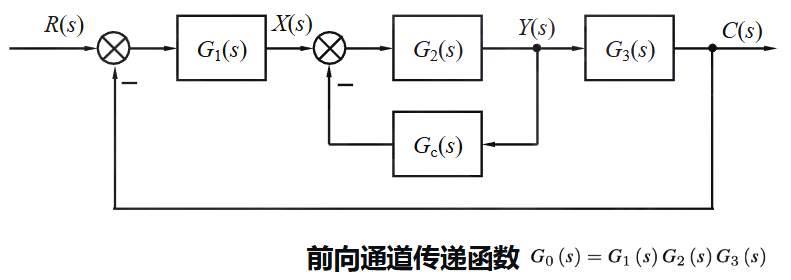
\includegraphics[width = .7\textwidth]{note/frequency correction/figure/3.png}
\end{center}

\begin{equation*}
    G(s) = \frac{G_0(s)}{1 + G_2(s) G_c(s)}
\end{equation*}
在满足$20\lg \left\lvert G_2(j\omega) G_c(j\omega) \right\rvert \ll 0$的频段，由上式可以看出此时校正系统的开环频率特性近似写为：
\begin{equation*}
    G(s) \approx G_0(s)
\end{equation*}
在满足$20\lg\left\lvert G_2(j\omega) G_c(j\omega) \right\rvert \gg 0 $的频段，由上式可以看出此时校正系统的开环频率特性近似写为
\begin{equation*}
    G(s) \approx \frac{G_0(s)}{G_2(s) G_c(s)}
\end{equation*}
这个式子可以等价写为：
\begin{equation*}
    G_2(s) G_c(s) \approx \frac{G_0(s)}{G(s)}
\end{equation*}
在反馈校正的过程中，应当注意两点：
\begin{enumerate}
    \item 在$20\lg\left\lvert G_2(j\omega) G_c(j\omega) \right\rvert > 0 $的受校正频段内，应当使$20\lg\left\lvert G_0(j\omega) \right\rvert > 20\lg\left\lvert G(j\omega) \right\rvert  $，这个式子大得越多，校正精度越高
    \item 局部反馈回路必须稳定
\end{enumerate}

\subsubsection{设计流程}

我们通过期望频率特性法来设计反馈校正：
\begin{enumerate}
    \item 按照稳态性能指标要求，绘制待校正系统的开环对数幅频特性$L_0(\omega)$
    \item 根据给定性能指标要求，绘制期望开环对数幅频特性$L(\omega)$
    \item 由下式求得$G_2(s) G_c(s)$的传递函数
    \begin{equation*}
        20 \lg \left\lvert G_2(j\omega) G_c(j\omega) \right\rvert = L_0(\omega) - L(\omega) 
    \end{equation*}
    \item 检验局部反馈回路的稳定性，并检查期望剪切频率附近$\left\lvert G_2(j\omega) G_c(j\omega) \right\rvert > 1 $的程度
    \item 由$G_2 G_c$求$G_c$
    \item 检验校正后系统的性能指标是否满足要求
\end{enumerate}

\chapterimage{15.jpg}
\chapter{基于根轨迹的校正}

\section{基本思想}

\subsection{性能指标的转换}

当性能指标以时域形式给出的时候，适合采用根轨迹法设计串联校正装置，给出的时域指标可能如下：
\begin{enumerate}
    \item 阻尼比$\xi$
    \item 自然振荡频率$\omega_n$
    \item 最大超调量$\sigma_p$
    \item 调整时间$t_s$
\end{enumerate}

设计时一般根据性能指标要求确定闭环主导极点，设计校正装置，使校正后的根轨迹通过期望的闭环主导极点

如果给定的期望指标是阻尼比和自然振荡频率，则闭环主导极点为：
\begin{equation*}
    s_{1,2} = - \xi \omega_n \pm j \omega_n \sqrt{1 - \xi^2}
\end{equation*}

如果给定超调量和调节时间，则可以通过以下的式子先算出期望的阻尼比和自然振荡频率，再算出闭环主导极点：
\begin{equation*}
    \begin{split}
        \sigma \% &= e^{-\frac{\pi \xi}{\sqrt{1-\xi^2}}}  \times 100 \%     \\
        t_s &= \frac{3.5}{\xi \omega_n}
    \end{split}
\end{equation*}

\subsection{零极点对根轨迹的影响}

零点对于根轨迹的影响如下图所示：
\begin{center}
    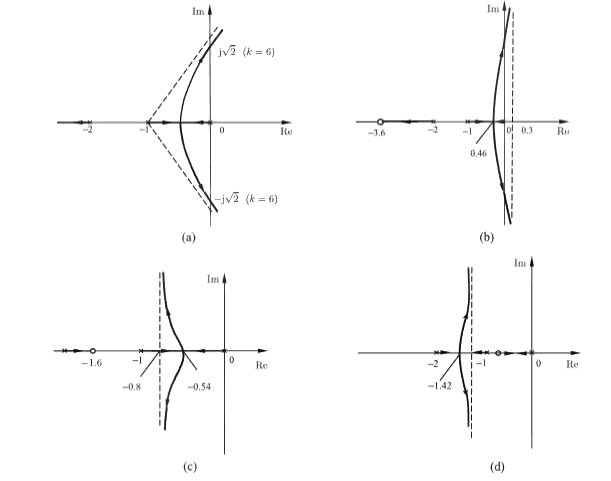
\includegraphics[width = .5\textwidth]{note/root locus correction/figure/1.png}
\end{center}
从图上可以看出添加一个零点可以使根轨迹向左或者右移动，或者使根轨迹反转

极点对于根轨迹的影响如下图所示：
\begin{center}
    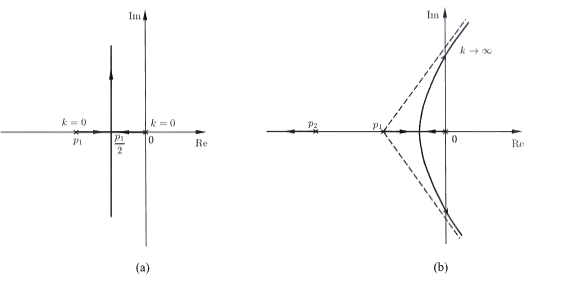
\includegraphics[width = .6\textwidth]{note/root locus correction/figure/2.png}
\end{center}

从图上可以看出添加一个极点可以使根轨迹向右移动

\subsection{超前环节}
超前环节的传递函数为
\begin{equation*}
    G_c(s) = K_c \frac{s-z_c}{s-p_c}  \quad  p_c < z_c < 0
\end{equation*}
引入超前环节之后相当于给原开环系统补充了一个零点和一个极点，同时超前环节会产生一个幅角：
\begin{equation*}
    \varphi_c = \varphi_z - \varphi_p > 0
\end{equation*}
$\varphi_c$不宜太大，否则难以实现

\textbf{超前环节会使系统根轨迹向左移动}

同时，引入超前环节相当于引入了一对开环偶极子，在加入偶极子之后，系统的开环增益发生了变化，适当选取偶极子可以增加系统的静态性能

\section{超前校正环节设计}

我们通过以下步骤，基于根轨迹进行超前校正的设计
\begin{enumerate}
    \item 根据性能指标要求，确定系统闭环主导极点$s_1$的期望位置
    \item 画出未校正系统的根轨迹，如果根轨迹通过闭环主导极点的期望位置，则简单调整开环增益即可产生期望的闭环极点；如果闭环主导极点的期望位置在根轨迹的左侧，则采用超前校正
    \item 对于期望的闭环主导极点$s_1$，按下面的式子确定超前校正环节应产生的幅角$\varphi$
    \begin{equation*}
        \varphi = (2l+1) 180^\circ - \angle G_0(s_1)
    \end{equation*}
    \item 按照下面式子确定超前校正环节的零点和极点：
    \begin{equation*}
        \angle(s_1-z_c) - \angle(s_1-p_c) = \varphi
    \end{equation*}
    \item 根据根轨迹幅值条件，按照下式确定超前校正环节的增益$K_c$
    \begin{equation*}
        K_c = \frac{\left\lvert z_c \right\rvert \left\lvert s_1 - p_c \right\rvert  }{\left\lvert G_0(s_1) \right\rvert \left\lvert p_c \right\rvert \left\lvert s_1 - z_c \right\rvert  }
    \end{equation*}
    进而确定超前校正环节的传递函数为：
    \begin{equation*}
        G_c(s) = K_c \alpha  \frac{s- z_c}{s - p_c}
    \end{equation*}
    \item 对于设计好的串联校正环节，检查校正后系统的动态性能指标是否满足设计要求。如果不满足，则需要调整主导极点的位置，重复上述设计过程
\end{enumerate}

对于超前校正环节零极点的确定，我们有以下几种方式：
\begin{enumerate}
    \item 给定具阻尼角为$\theta$的主导极点$s_1$，若超前环节在$s_1$处提供的超前角为$\varphi$，则超前环节的一组零极点由下式确定：
    \begin{equation*}
        \begin{cases}
            p_c &= -\left\lvert s_1 \right\rvert \frac{\cos \frac{1}{2}(\varphi - \theta)}{\cos \frac{1}{2} (\theta + \varphi)}  \\
            z_c &= -\left\lvert s_1 \right\rvert \frac{\cos \frac{1}{2}(\varphi + \theta)}{\cos \frac{1}{2} (\varphi - \theta)}
        \end{cases}
    \end{equation*}
    \item 给定复平面第二象限的点$s_1$和角度$\varphi$，而$p_c < z_c$是负实轴上使$\angle z_c s_1 p_c = \varphi$的两个动点。令$\angle z_c O s_1 = \theta$，则当$\angle O s_1 z_c = \frac{1}{2} (180^\circ - \theta -\varphi)$时，比值$\alpha = \frac{\left\lvert p_c \right\rvert }{\left\lvert z_c \right\rvert }$最小，且最小值$\alpha_{min}$为
    \begin{equation*}
        \alpha_{min} = 1 + \frac{2 \sin \theta \sin \varphi}{\cos (\theta + \varphi) + 1}
    \end{equation*}
    \item 幅值确定法：首先我们可以根据以下的式子算出$\angle z_c s_1 O = \eta $：
    \begin{equation*}
        \begin{split}
            \frac{1}{\tan \eta} &= \alpha \frac{\left\lvert s_1 - z_c \right\rvert}{\left\lvert s_1 - p_c \right\rvert } \frac{1}{\sin \varphi} - \frac{1}{\tan \varphi} \\
            &\alpha \frac{\left\lvert s_1 - z_c \right\rvert}{\left\lvert s_1 - p_c \right\rvert } = \frac{M}{k} \\
            M &= \frac{\left\lvert s_1^v \right\rvert \prod_{i=1}^{n-v}\left\lvert s_1 - p_i \right\rvert}{\prod_{j=1}^{m}\left\lvert s_1 - z_j \right\rvert}
        \end{split}
    \end{equation*}
    在算出$\eta$之后可以由角度关系求得：
    \begin{equation*}
        \begin{split}
            \left\lvert z_c \right\rvert &= \omega_n \frac{\sin \eta}{\sin \delta} \\
            \left\lvert p_c \right\rvert &= \omega_n \frac{\sin (\theta + \eta)}{\sin (\delta - \varphi)} \\
        \end{split}
    \end{equation*}
\end{enumerate}

\subsection{迟后校正环节设计}

我们可以通过以下步骤，设计基于根轨迹的迟后校正：
\begin{enumerate}
    \item 用原系统的开环传递函数$G_0(s)$做出原系统的根轨迹，确定调整开环增益可以使原系统的动态性能满足设计指标
    \item 在原系统的根轨迹上确定闭环主导极点$s_1$，并求出点$s_1$对应的开环增益$K_0$
    \item 根据控制系统的设计要求，求出满足稳态误差设计指标的开环增益$K$，即校正以后应有的开环增益
    \item 为了使点$s_1$的开环增益$K_0$增大到$K$，则有：
    \begin{equation*}
        \beta = \frac{K}{K_0}
    \end{equation*}
    按照串联迟后校正的条件，极点$p_c$和零点$z_c$应充分接近并靠近原点，按照
    \begin{equation*}
        \beta = \frac{z_c}{p_c}
    \end{equation*}
    可以确定校正环节的零极点值。至此，串联迟后校正环节的参数全部计算完成
    \item 绘制出校正后的根轨迹图，检验系统的动态性能指标和静态稳态性能指标
\end{enumerate}

\subsection{迟后-超前校正环节的设计}

我们可以通过以下步骤，设计基于根轨迹的迟后-超前校正环节：
\begin{enumerate}
    \item 根据期望性能指标要求，确定满足要求的闭环主导极点的候选区域
    \item 确定超前部分：作出校正前系统的根轨迹。若根轨迹未穿过候选区域，则修改初选期望闭环出到极点的位置。合理选择超前校正零极点，使其穿过期望主导极点
    \item 校验系统响应动态性能是否满足要求，不满足则可适当右移校正环节的零点和（或）左移其极点，使系统根轨迹进一步左移，绘制响应根轨迹，并重新选择裕度更大的闭环系统主导极点。
    \item 确定迟后部分：对新选主导极点，按幅值条件求出校正后系统的根轨迹增益$k$以及静态误差系数，检验系统稳态精度是否满足要求。若不满足要求，则根据稳态误差要求确定迟后校正零极点位置
    \item 迟后校正后，原主导极点位置可能发生变化。此时，应绘制迟后超前校正后系统根轨迹，判断系统动、静态性能是否满足要求。
\end{enumerate}

\subsection{反馈校正的设计}

我们可以通过以下步骤，设计基于根轨迹的局部反馈校正：
\begin{enumerate}
    \item 做出未进行局部反馈的原系统的根轨迹。
    \item 求出满足设计要求的闭环主导极点的位置$s_1$和$s_2$
    \item 在系统的开环极点中，找出系统改变位置的开环极点$p_c$，当改变$p_c$的位置时，可以使根轨迹通过$s_1$和$s_2$点
    \item 检验围绕$p_c$是否可以建立局部反馈。即在实际问题中，$p_c$所在的原件的输出变量是否可以测量；$p_c$所在原件的输入变量是否可以实现相加
    \item 为使闭环主导极点达到$s_1$和$s_2$，按照根轨迹的复制条件，求出极点$p_c$的希望位置$\overline{p}_c$
    \item 求出使小闭环的闭环极点成为$\overline{p}_c$的条件，从而确定小闭环的参数
    \item 对于大闭环，求出主导极点$s_1$和$s_2$所对应的开环增益$K$，调整大回路中的放大倍数，使大闭环的主导极点为$s_1$和$s_2$
    \item 进行必要的验算
\end{enumerate}

\chapterimage{16.jpg}
\chapter{PID控制器}

\section{PID控制器概述与其基本作用}

\subsection{比例控制器}

一个比例控制器的例子如下：
\begin{center}
    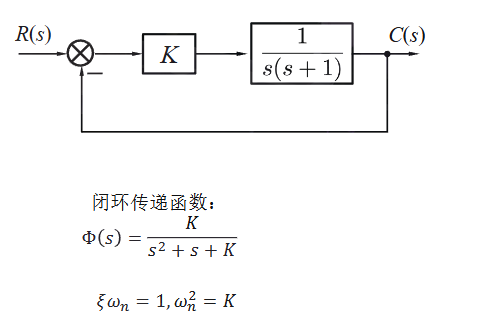
\includegraphics[width = .5\textwidth]{note/PID design/figure/1.png}
\end{center}

\textbf{比例控制器有以下的优点：}
\begin{enumerate}
    \item 提高系统稳态精度
    \item 提高系统的快速性
    \item 降低稳定裕度
\end{enumerate}

\subsection{PD控制器}

一个PD控制器的例子如下：
\begin{center}
    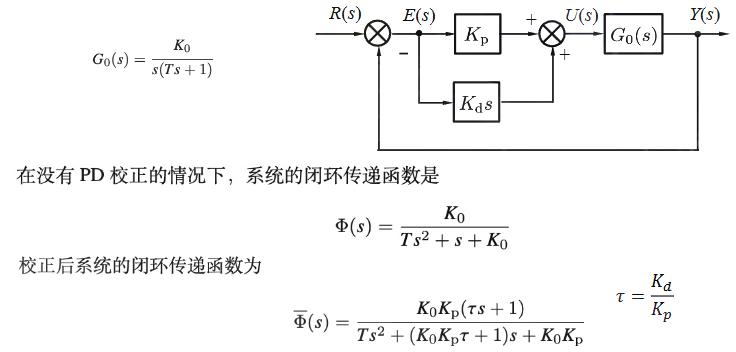
\includegraphics[width = .5\textwidth]{note/PID design/figure/2.png}
\end{center}

\textbf{PD控制器有以下优点：}
\begin{enumerate}
    \item 改变系统的自然震荡频率和阻尼比
    \item 提高系统的动态性能，加快响应速度，提高系统的稳定性
\end{enumerate}

\subsection{PI控制器}

PI控制器的一般形式如下：
\begin{center}
    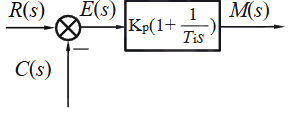
\includegraphics[width = .3\textwidth]{note/PID design/figure/3.png}
\end{center}

PI控制器相当于积分环节和一阶微分环节串联，几分环节改变系统型别，一阶微分环节系统的自然频率和阻尼比，保证闭环系统的稳定性，所以\textbf{PI控制器有以下的优点：}
\begin{enumerate}
    \item 提高系统的型别
    \item 提高系统的动态性能
\end{enumerate}

\textbf{
\begin{itemize}
    \item 对于单一的积分控制器，可以提高系统的型别，以消除或减弱稳态误差
    \item 如果系统不可变部分已有积分环节，再采用单一的积分控制可能导致系统不稳定，故此时可以引入PI控制器
    \item PI控制通过在原点增加极点来"消灭"稳态误差，但是代价是把根轨迹向右“挤”，如果积分作用太强($T_i$太小)，系统超调会猛增，甚至失控
\end{itemize}
}

\subsection{PID控制器}

PID控制器的一般形式如下：
\begin{center}
    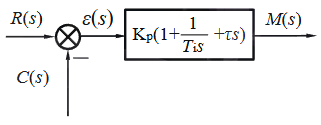
\includegraphics[width = .3\textwidth]{note/PID design/figure/4.png}
\end{center}

\textbf{PID控制器具有以下的优点：}
\begin{enumerate}
    \item 提高系统的型别
    \item 通过合适选择参数，还将为系统增加两个开环零点，在提高系统动态性能方面具有更大的优越性
\end{enumerate}

\section{PID参数整定}

\subsection{动态响应法}
以传递函数为$G(s) = \frac{K e^{-\tau s}}{Ts + 1}$为例来介绍这种方法，具体步骤如下：
\begin{enumerate}
    \item 求取动态阶跃响应曲线，求得如下：
    \begin{center}
        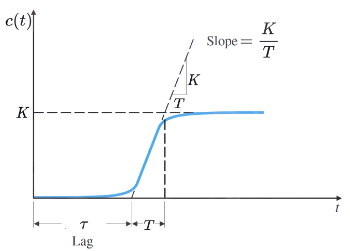
\includegraphics[width = .4\textwidth]{note/PID design/figure/5.png}
    \end{center}
    \item 估计被控对象的传递函数，将其拐点切线和时间轴和$c(t) = K$的交点可得到$\tau$和$T$的值，如上图所示
    \item 由Ziegler-Nichols给出的调整法则表，确定PID参数，具体如下：
    \begin{center}
        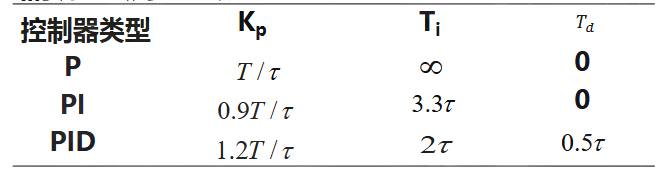
\includegraphics[width = .4\textwidth]{note/PID design/figure/6.png}
    \end{center}
    \item 由上表可以确定控制器的具体传递函数，根据选用P/PI/PID控制器而定
\end{enumerate}

使用动态响应法有几点注意事项：
\begin{enumerate}
    \item 系统开环下测出阶跃响应
    \item 闭环单位阶跃响应为S形
    \item 这种方法能保证阶跃响应的暂态分量最大峰值和第二峰值之比为4:1，$\xi \approx 0.21$
    \item \textbf{被控对象有几分环节和复数极点时不适用}
\end{enumerate}

\subsection{临界增益法}

\textbf{临界增益法在系统闭环情况下进行}，示意图如下：
\begin{center}
    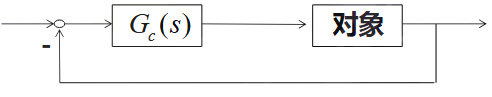
\includegraphics[width = .5\textwidth]{note/PID design/figure/7.png}
\end{center}

具体步骤如下：
\begin{enumerate}
    \item 令$I_i = \infty , T_d = 0$，将控制器设置为比例控制，将$K_p$从0增大，首次出现等幅振荡时，记下此时的增益$K_{ps}$和振荡周期$T_s$
    \item 根据Ziegler-Nichols给出的调整法则表，确定PID参数，具体如下：
    \begin{center}
        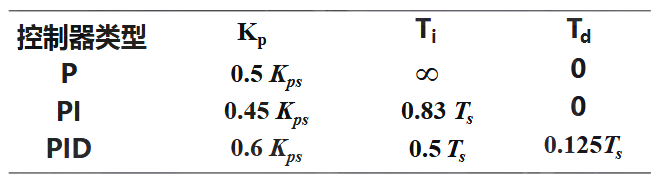
\includegraphics[width = .3\textwidth]{note/PID design/figure/8.png}
    \end{center}
\end{enumerate}

\textbf{以上两种方法均用到了Z-N法给出的参数，但是这个参数往往会让超调$>60\%$，在实际工程中，我们需要手动微调PID零点位置，来压低超调量}

\section{离散PID}

\begin{center}
    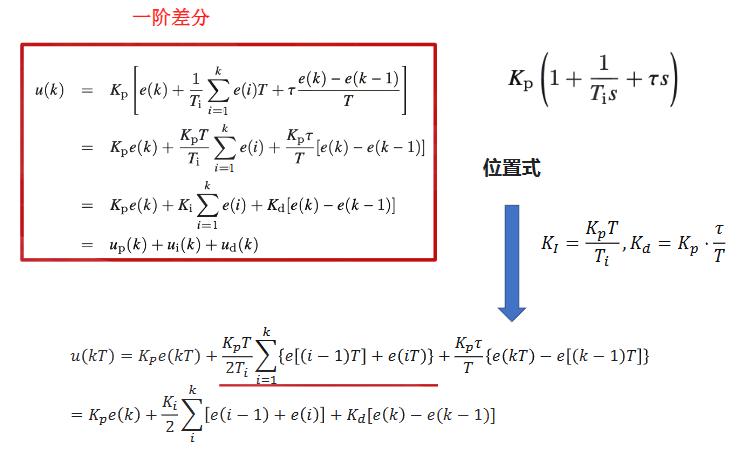
\includegraphics[width = .6\textwidth]{note/PID design/figure/9.png} \\
    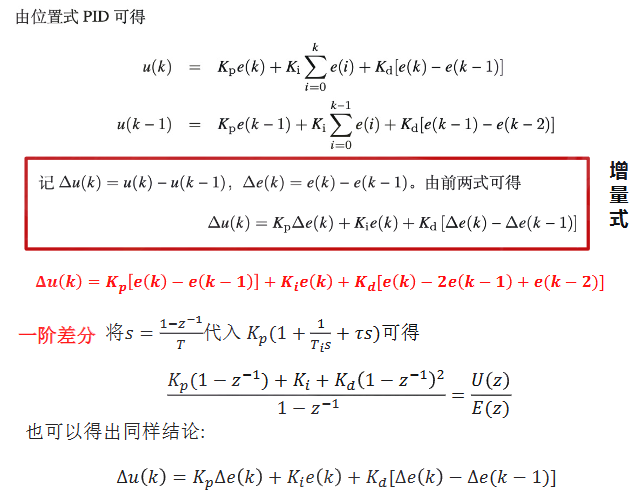
\includegraphics[width = .6\textwidth]{note/PID design/figure/10.png} \\
    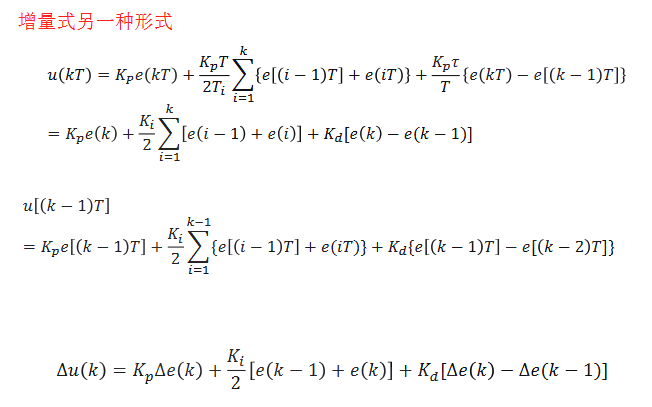
\includegraphics[width = .6\textwidth]{note/PID design/figure/11.png}
\end{center}


\chapterimage{17.jpg}
\chapter{离散系统的校正}

\section{模拟化设计}

\subsection{校正思路}

我们通过以下步骤，采用模拟化校正设计校正环节：
\begin{enumerate}
    \item 根据指标，考虑零阶保持器的影响（零阶保持器在离散化后对系统的影响可以近似为一个惯性环节），用连续系统理论设计校正装置$D(s)$
    \item 对$D(s)$进行离散化，确定数字校正装置的脉冲传递函数$D(z)$
    \item 检查离散控制系统的性能是否满足要求
    \item 写出$D(z)$的差分方程（递推形式），编制程序实现的控制规律
    \item 检验设计的正确性
\end{enumerate}

\subsection{连续控制器的离散化方法}

\subsubsection{阶跃响应不变法}

阶跃响应不变法主要表现为以下的形式：

具有零阶保持其的连续对象在单位阶跃序列$1^{*}(t)$作用下的输出，等于连续对象在单位阶跃信号$1(t)$作用下的输出

\subsubsection{替换法}

替换法的基本思想为：对于给定的连续系统传递函数$D(s)$，设法找到$s$域到$z$域的某种映射关系，它将$s$域的变量映射到$z$平面上，由此得到与连续系统传递函数$D(s)$相对应的离散传递函数$D(z)$，常见的替换法有一阶差分近似和双线性变换，具体方法如下：
\begin{enumerate}
    \item 一阶差分：用一阶差分近似导数：
    \begin{itemize}
        \item 后向差分方程：$s = \frac{1-z^{-1}}{T}$，变换后系统仍然稳定
        \item 前向差分方程：$s = \frac{z-1}{T}$，变换后系统可能不稳定
    \end{itemize}
    \item 双线性变换：$s = \frac{2}{T}\frac{1-z^{-1}}{1+z^{-1}}$
    \item 根匹配法：$s+a \rightarrow 1 - e^{-aT} z^{-1}$，匹配完零极点之后需要确定数字控制器增益$K_z$，可以通过以下的方式确定：
    \begin{itemize}
        \item 使数字控制器与模拟控制器在低频处增益一致
        \item 使某类典型输入下的稳态误差保持一致
        \item 根据题目指定的性能指标要求确定
    \end{itemize}
    \item 冲激响应不变法：$D(z) = Z[D(s)]$
\end{enumerate}

具体举例如下：
\begin{center}
    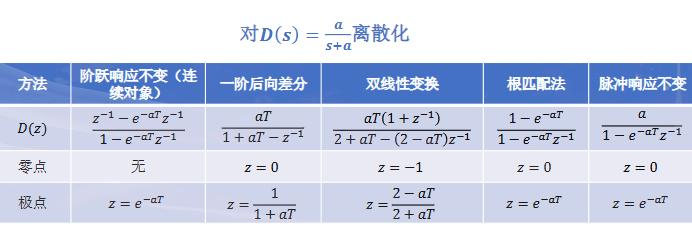
\includegraphics[width = .6\textwidth]{note/discrete system correction/figure/1.png}
\end{center}


\section{离散化设计}

\subsection{设计思路}

离散化的设计采用期望特性校正法，步骤如下：
\begin{center}
    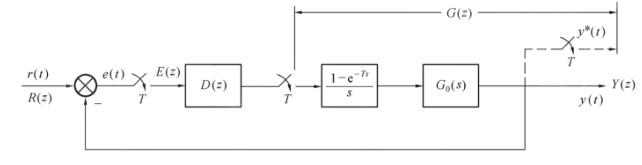
\includegraphics[width = .6\textwidth]{note/discrete system correction/figure/2.png}
\end{center}

一般的单位负反馈系统如下，$D(z)$是我们要设计的校正装置，我们将设计期望的$\Phi(z)$和$\Phi_e(z)$，用以下的式子确定校正装置$D(z)$
\begin{equation*}
    \begin{split}
        \Phi(z) = \frac{G(z)D(z)}{1+G(z)D(z)},&\Phi_e(z) = \frac{1}{1+G(z)D(z)} = 1 - \Phi(z)  \\
        &G(z)D(z) = \frac{\Phi(z)}{\Phi_e(z)} \\
        &D(z) = \frac{\Phi(z)}{\Phi_e(z)G(z)}  \\
    \end{split}
\end{equation*}

同时，在离散化设计的过程中，要遵循\textbf{最少拍设计}，具体为：\textbf{对典型信号能在有限拍内结束过渡过程，同时要在最少的拍内结束过渡过程}

由最小拍设计，我们可以得到以下的几个结论：
\begin{enumerate}
    \item 闭环误差传递函数的形式一定为：$\Phi_e(z) = (1 - z^{-1})^r F(z)$，$r$为输入信号Z变换后分母的关于$1-z^{-1}$的阶次
    \item $E(z) = F(z)A(z)$关于$z^{-1}$的阶次是有限的，且为最小，即$F(z)$关于$z^{-1}$的阶次最小
\end{enumerate}

\subsubsection{广义脉冲传递函数不含纯延迟环节和单位圆上和圆外的零极点}

此时$F(z) = 1$，$\Phi(z) = (1-z^{-1})^r$，$\Phi(z) = 1 - (1 - z^{-1})^r$，在输入为不同的信号的时候得到的调整时间如下表所示：
\begin{center}
    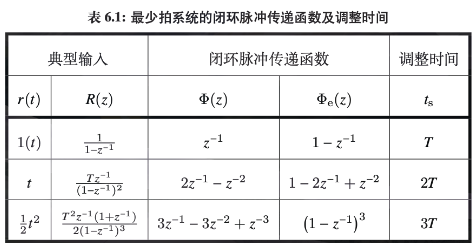
\includegraphics[width = .6\textwidth]{note/discrete system correction/figure/3.png}
\end{center}

\subsubsection{广义脉冲传递函数有纯延迟环节}

此时$G(z) = G_1(z) z^{-L}$，若想要用$D(z)$抵消掉$G(z)$中的纯延迟项，此时$D(z)$会出现超前项，这违背了因果性，在物理上不可实现

所以我们可以得出一个结论：\textbf{若$G(z)$含有纯延迟环节$z^{-L}$，则闭环传递函数$\Phi(z)$也至少包含相同的延迟因子$z^{-L}$}

\subsubsection{广义脉冲传递函数含有单位圆上和圆外的零极点}

若$G(z)$有单位圆上及圆外的零极点，如果不加处理，会造成$D(z)$含单位圆上及圆外的零极点，这样会导致控制器$D(z)$不稳定

所以，我们需要设计$\Phi(z)$和$\Phi_e(z)$，满足以下的要求：
\begin{enumerate}
    \item 闭环传递函数$\Phi(z)$应包含$G(z)$在单位圆上和圆外的零点
    \item 误差传递函数$\Phi_e(z)$应包含$G(z)$在单位圆上和圆外的极点
    \item $\Phi(z)$和$\Phi_e(z)$关于$z^{-1}$的阶次应当相同，且为多项式
\end{enumerate}

\textbf{注意：此设计方法设计出来的校正装置只适用于使用的典型输入信号，对于其他的典型输入信号并不适用！}

\subsubsection{最少拍系统产生纹波的原因}

在经过二拍之后，零阶保持器的输入序列并不是常值脉冲，而是围绕平均值上下波动，从而保持器的输出电压在二拍以后也围绕平均值波动，产生输出纹波。

因此，\textbf{无纹波输出要求序列在有限个采样周期后达到相对稳定}


\partsimage{cov18.pdf}
\part{非线性系统}

\chapterimage{7.jpg}
\chapter{非线性控制系统分析}

\section{非线性特性}

\subsection{非线性特点}

非线性和线性系统的区别很大，其特点主要体现在以下的几点：
\begin{enumerate}
    \item 不满足叠加定理
    \item 其稳定性的分析更加复杂，系统的初值对于稳定性的影响比较大
    \item 在非线性系统中，存在自激振荡，表现为振荡特性，且在振幅较大的时候会慢慢振幅变小，在振幅较小的时候会慢慢变大
    \item 混沌现象：有些非线性系统的输出对初始条件极为铭感。即使具有确定性的、十分精确的模型，也不能语言系统初始条件变化时的输出变化，这个现象就被称为混沌现象
\end{enumerate}

\subsection{典型非线性特性}

我们主要讨论以下几种比较典型的非线性特性：
\begin{enumerate}
    \item 饱和特性
    \item 死区特性
    \item 滞环特性
    \item 继电特性
    \item 变增益特性
\end{enumerate}
\subsubsection{饱和特性}

饱和特性的示意图如下：
\begin{center}
    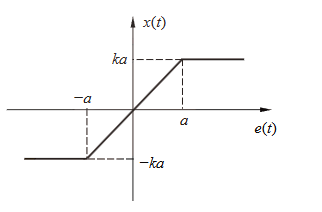
\includegraphics[width = .2\textwidth]{note/nonlinear system/figure/1.png}
\end{center}

其表达式可以写成以下的形式：
\[
x(t)=
\begin{cases}
k e(t), & |e(t)| \le a,\\
k a \operatorname{sgn}(e(t)), & |e(t)| > a.
\end{cases}
\]

\subsubsection{死区特性}

死区特性的示意图如下：
\begin{center}
    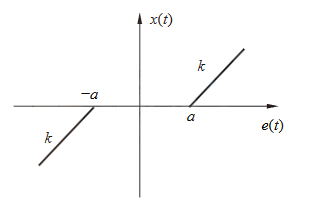
\includegraphics[width = .2\textwidth]{note/nonlinear system/figure/2.png}
\end{center}

其表达式可以写成以下的形式：
\[
x(t)=
\begin{cases}
k\bigl(e(t)+a\bigr), & e(t)<-a,\\
0, & |e(t)|<a,\\
k\bigl(e(t)-a\bigr), & e(t)>a.
\end{cases}
\]

\subsubsection{滞环特性}

滞环特性的示意图如下：
\begin{center}
    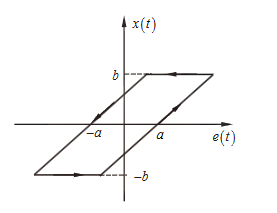
\includegraphics[width = .2\textwidth]{note/nonlinear system/figure/3.png}
\end{center}

其表达式可以写成以下的形式：
\[
x(t)=
\begin{cases}
k\bigl[e(t)-a\bigr], & \dot{x}(t)>0,\\
b\operatorname{sgn}\bigl(e(t)\bigr), & \dot{x}(t)=0,\\
k\bigl[e(t)+a\bigr], & \dot{x}(t)<0.
\end{cases}
\]

\subsubsection{继电特性}

继电特性的示意图如下：
\begin{center}
    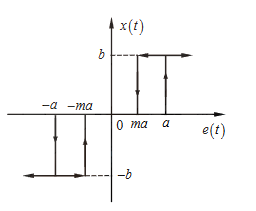
\includegraphics[width = .2\textwidth]{note/nonlinear system/figure/4.png}
\end{center}

其表达式可以写成以下的形式：
\[
x(t)=
\begin{cases}
0, & -ma < e(t) < a,\ \dot{e}(t)>0,\\
0, & -a < e(t) < ma,\ \dot{e}(t)<0,\\
b\operatorname{sgn}\bigl(e(t)\bigr), & |e(t)| \ge a,\\
b, & e(t) \ge ma,\ \dot{e}(t)<0,\\
-b, & e(t) \le -ma,\ \dot{e}(t)>0.
\end{cases}
\]

可以发现，这里面$m$和$a$对于特性的影响比较大，当$m$和$a$分别取特定值的时候可以得到以下的几种特殊情况：
\begin{enumerate}
    \item 当$a = 0$时可以得到理想继电器：
    \begin{center}
        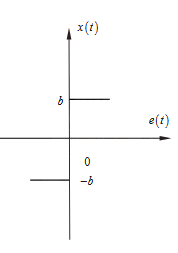
\includegraphics[width = .2\textwidth]{note/nonlinear system/figure/5.png}
    \end{center}
    \item 当$m = 1$时可以得到带死区的继电器：
    \begin{center}
        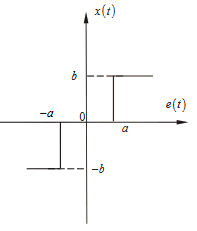
\includegraphics[width = .2\textwidth]{note/nonlinear system/figure/6.png}
    \end{center}
    \item 当$m = -1$时可以得到带滞环的继电器：
    \begin{center}
        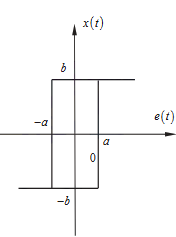
\includegraphics[width = .2\textwidth]{note/nonlinear system/figure/7.png}
    \end{center}
\end{enumerate}

\subsubsection{变增益特性}

变增益特性的示意图如下：
\begin{center}
    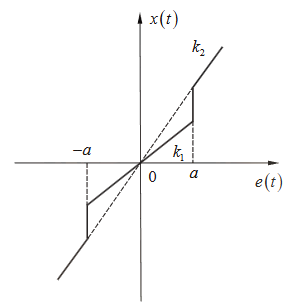
\includegraphics[width = .2\textwidth]{note/nonlinear system/figure/8.png}
\end{center}

其表达式可以写成以下形式：
\[
x(t)=
\begin{cases}
k_1 e(t), & |e(t)| < a,\\
k_2 e(t), & |e(t)| > a.
\end{cases}
\]

\section{描述函数法}

对于一个线性系统，我们可以通过写出其传递函数来给出输入和输出的具体关系，通过输入来计算输出。可是，对于非线性系统，我们没有办法直接写出其传递函数，此时应该怎么办呢？

我们可以通过类比线性系统\hyperref[frequency-characteristics]{频率特性}来给出非线性系统的近似的传递函数，具体如下：

假设一个时不变系统如下图所示：
\begin{center}
    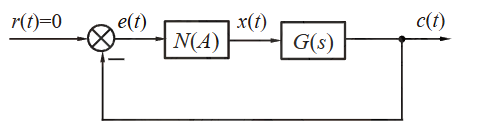
\includegraphics[width = .4\textwidth]{note/nonlinear system/figure/9.png}
\end{center}
且系统的误差为$e(t) = A \sin \omega t$，此时经过非线性部分之后得到的输出一定为周期信号（输入经过时不变系统不改变周期性），故我们可以通过Fourier级数展开将$x(t)$写成如下的形式：
\[
\begin{aligned}
x(t) &= A_0 + \sum_{n=1}^{\infty}
\left(A_n \cos n\omega t + B_n \sin n\omega t\right) \\
&= A_0 + \sum_{n=1}^{\infty}
X_n \sin\left(n\omega t + \varphi_n\right)
\end{aligned}
\]
其中：
\[
\begin{aligned}
A_0 &= \frac{1}{2\pi}\int_{0}^{2\pi} x(t)\,\mathrm{d}(\omega t) \\
A_n &= \frac{1}{\pi}\int_{0}^{2\pi} x(t)\cos n\omega t\,\mathrm{d}(\omega t) \\
B_n &= \frac{1}{\pi}\int_{0}^{2\pi} x(t)\sin n\omega t\,\mathrm{d}(\omega t) \\
X_n &= \sqrt{A_n^2+B_n^2} \\
\varphi_n &= \arctan \frac{A_n}{B_n}
\end{aligned}
\]
但此时的输出仍然很复杂，且有很多谐波叠加，为了写成类似频率特性的形式，我们引入以下两个假设，使其近似为频率特性的形式：
\begin{enumerate}
    \item \textbf{奇对称性}：即正弦输入下的输出$x(t)$为$t$的奇对称函数，$x(t + \frac{\pi}{\omega}) = - x(t)$，以保证非线性环节的正弦响应不含有常值分量，即$A_0 = 0$

    进一步地，若$x(t)$为奇函数，此时我们可以得到$A_i = 0, B_1 = \frac{4}{\pi}\int_0^{\frac{\pi}{2}} x(t) \sin \omega t d \omega t$
    \item \textbf{线性环节低通滤波特性良好}：在整个系统中，线性环节低通滤波特性良好，意味着在正弦输入情况下，实际输出中高次谐波分量将被大大削弱。只有在这种条件下，实际输出中基波分量才能较精确地近似代替正弦输入信号下的实际输出。当然，描述函数法分析的精度也直接取决于线性环节的低通滤波特性，低通滤波特性越好，相应的分析精度也越高。
\end{enumerate}
有了以上两个假设，我们可以将非线性环节的输出写成以下的形式：
\[
\begin{aligned}
x(t) \approx x_1(t)
&= A_1 \cos \omega t + B_1 \sin \omega t \\
&= X_1 \sin\left(\omega t+\varphi_1\right)
\end{aligned}
\]
此时非线性环节的描述函数为：
\[
\begin{aligned}
N(A)
&= \frac{X_1}{A} e^{j\varphi_1} \\
&= \frac{\sqrt{A_1^2+B_1^2}}{A}
e^{j\arctan\frac{A_1}{B_1}} \\
&= \frac{B_1}{A} + j\frac{A_1}{A}
\end{aligned}
\]

\subsection{典型非线性特性的描述函数}

\subsubsection{理想继电特性}
为了更好地看出$x(t)$的图像，我们将$e(t)$的图像竖直放在$x(e)$的下方，如下图所示：
\begin{center}
    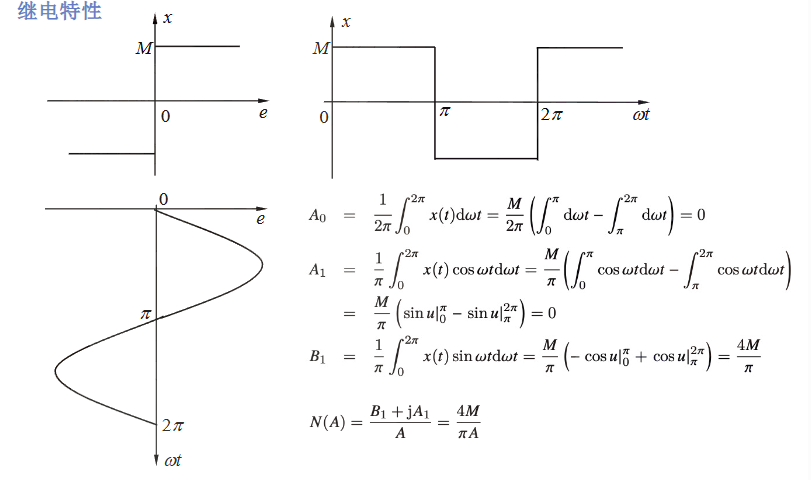
\includegraphics[width = .5\textwidth]{note/nonlinear system/figure/10.png}
\end{center}
由图可知：
\[
\begin{aligned}
A_0
&= \frac{1}{2\pi}\int_{0}^{2\pi} x(t)\,\mathrm{d}\omega t
= \frac{M}{2\pi}\left(\int_{0}^{\pi}\mathrm{d}\omega t
-\int_{\pi}^{2\pi}\mathrm{d}\omega t\right)=0 \\
A_1
&= \frac{1}{\pi}\int_{0}^{2\pi} x(t)\cos\omega t\,\mathrm{d}\omega t
= \frac{M}{\pi}\left(\int_{0}^{\pi}\cos\omega t\,\mathrm{d}\omega t
-\int_{\pi}^{2\pi}\cos\omega t\,\mathrm{d}\omega t\right) \\
&= \frac{M}{\pi}\left(\sin\omega t\big|_{0}^{\pi}
-\sin\omega t\big|_{\pi}^{2\pi}\right)=0 \\
B_1
&= \frac{1}{\pi}\int_{0}^{2\pi} x(t)\sin\omega t\,\mathrm{d}\omega t
= \frac{M}{\pi}\left(-\cos\omega t\big|_{0}^{\pi}
+\cos\omega t\big|_{\pi}^{2\pi}\right)
= \frac{4M}{\pi} \\
N(A)
&= \frac{B_1+jA_1}{A}
= \frac{4M}{\pi A}
\end{aligned}
\]

\subsubsection{死区特性}
同样的，也可以给出示意图如下：
\begin{center}
    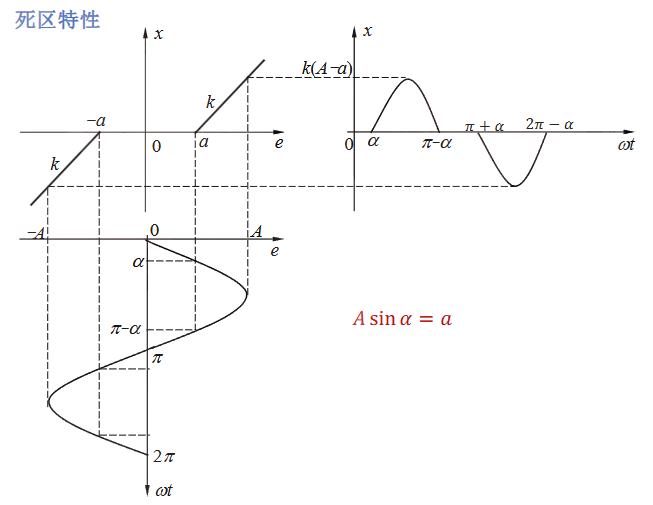
\includegraphics[width = .5\textwidth]{note/nonlinear system/figure/11.png}
\end{center}
由图：由于 $x(t)$ 为单位且奇对称的，并且 $x(t)\sin\omega t$ 具有 $1/4$ 波对称性，
所以有 $A_0=0, A_1=0$，并且
\[
\begin{aligned}
B_1
&= \frac{1}{\pi}\int_{0}^{2\pi} x(t)\sin\omega t\,\mathrm{d}(\omega t) \\
&= \frac{4}{\pi}\int_{\alpha}^{\frac{\pi}{2}}
k\left(A\sin\omega t-a\right)\sin\omega t\,\mathrm{d}(\omega t) \\
&= \frac{2kA}{\pi}
\left[
\frac{\pi}{2}
-\arcsin\frac{a}{A}
-\frac{a}{A}\sqrt{1-\left(\frac{a}{A}\right)^2}
\right],
\qquad A>a
\end{aligned}
\]

此时，可得死区特性的描述函数为
\[
N(A)=\frac{B_1}{A}
=\frac{2k}{\pi}
\left[
\frac{\pi}{2}
-\arcsin\frac{a}{A}
-\frac{a}{A}\sqrt{1-\left(\frac{a}{A}\right)^2}
\right],
\qquad A\ge a
\]

\subsubsection{饱和特性}
饱和特性的示意图如下：
\begin{center}
    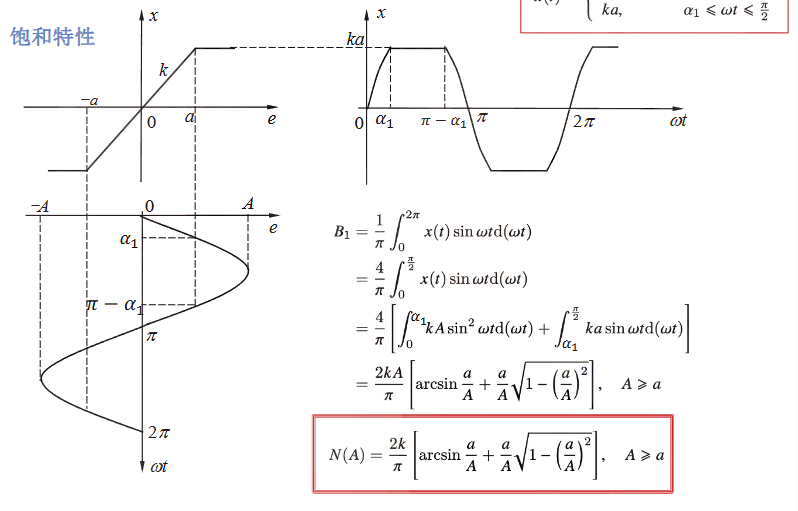
\includegraphics[width = .5\textwidth]{note/nonlinear system/figure/12.png}
\end{center}
由图可知：
\[
\begin{aligned}
A_1 & = A_0 = 0\\
B_1
&= \frac{1}{\pi}\int_{0}^{2\pi} x(t)\sin\omega t\,\mathrm{d}(\omega t) \\
&= \frac{4}{\pi}\int_{0}^{\frac{\pi}{2}} x(t)\sin\omega t\,\mathrm{d}(\omega t) \\
&= \frac{4}{\pi}
\left[
\int_{0}^{\alpha_1} kA\sin^2\omega t\,\mathrm{d}(\omega t)
+\int_{\alpha_1}^{\frac{\pi}{2}} ka\sin\omega t\,\mathrm{d}(\omega t)
\right] \\
&= \frac{2kA}{\pi}
\left[
\arcsin\frac{a}{A}
+\frac{a}{A}\sqrt{1-\left(\frac{a}{A}\right)^2}
\right],
\qquad A\ge a
\end{aligned}
\]

\[
N(A)=\frac{2k}{\pi}
\left[
\arcsin\frac{a}{A}
+\frac{a}{A}\sqrt{1-\left(\frac{a}{A}\right)^2}
\right],
\qquad A\ge a
\]

\subsubsection{滞环特性}
滞环特性的示意图如下：
\begin{center}
    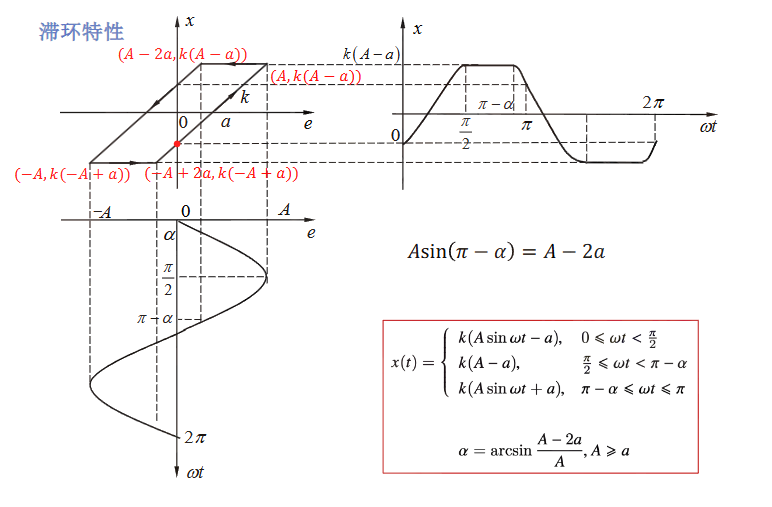
\includegraphics[width = .5\textwidth]{note/nonlinear system/figure/13.png}
\end{center}

由图：
\[
\begin{aligned}
A_1
&= \frac{1}{\pi}\int_{0}^{2\pi} x(t)\cos\omega t\,\mathrm{d}(\omega t) \\
&= \frac{2}{\pi}
\left[
\int_{0}^{\frac{\pi}{2}} k(A\sin\omega t-a)\cos\omega t\,\mathrm{d}(\omega t)
+\int_{\frac{\pi}{2}}^{\pi-\alpha} k(A-a)\cos\omega t\,\mathrm{d}(\omega t)\right. \\
&\qquad\left.
+\int_{\pi-\alpha}^{\pi} k(A\sin\omega t+a)\cos\omega t\,\mathrm{d}(\omega t)
\right] \\
&= \frac{4ka}{\pi}\left(\frac{a}{A}-1\right),
\qquad A\ge a
\end{aligned}
\]

\[
\begin{aligned}
B_1
&= \frac{1}{\pi}\int_{0}^{2\pi} x(t)\sin\omega t\,\mathrm{d}(\omega t) \\
&= \frac{2}{\pi}
\left[
\int_{0}^{\frac{\pi}{2}} k(A\sin\omega t-a)\sin\omega t\,\mathrm{d}(\omega t)
+\int_{\frac{\pi}{2}}^{\pi-\alpha} k(A-a)\sin\omega t\,\mathrm{d}(\omega t)\right. \\
&\qquad\left.
+\int_{\pi-\alpha}^{\pi} k(A\sin\omega t+a)\sin\omega t\,\mathrm{d}(\omega t)
\right] \\
&= \frac{kA}{\pi}
\left[
\frac{\pi}{2}
+\arcsin\left(1-\frac{2a}{A}\right)
+2\left(1-\frac{2a}{A}\right)
\sqrt{\frac{a}{A}\left(1-\frac{a}{A}\right)}
\right],
\qquad A\ge a
\end{aligned}
\]

\[
\begin{aligned}
N(A)
&= \frac{B_1}{A}+j\frac{A_1}{A} \\
&= \frac{k}{\pi}
\left[
\frac{\pi}{2}
+\arcsin\left(1-\frac{2a}{A}\right)
+2\left(1-\frac{2a}{A}\right)
\sqrt{\frac{a}{A}\left(1-\frac{a}{A}\right)}
\right] \\
&\qquad
+j\frac{4ka}{\pi A}\left(\frac{a}{A}-1\right),
\qquad A\ge a
\end{aligned}
\]

\subsubsection{继电特性}
继电特性的示意图如下：
\begin{center}
    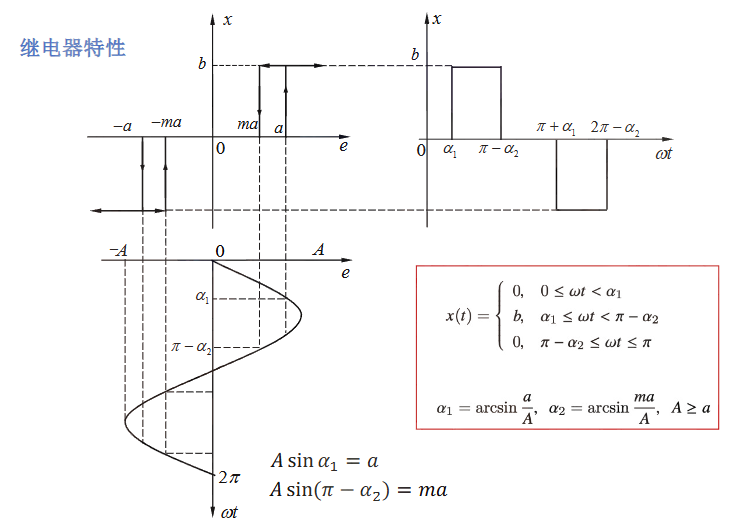
\includegraphics[width = .5\textwidth]{note/nonlinear system/figure/14.png}
\end{center}
由 $x(t)$ 正、负半波对称性知，$A_0=0$。计算 $A_1$，$B_1$ 得
\[
\begin{aligned}
A_1
&= \frac{1}{\pi}\int_{0}^{2\pi}x(t)\cos\omega t\,\mathrm{d}(\omega t) \\
&= \frac{2}{\pi}\int_{\alpha_1}^{\pi-\alpha_2} b\cos\omega t\,\mathrm{d}(\omega t) \\
&= \frac{2ab}{\pi A}(m-1),
\qquad A\ge a
\end{aligned}
\]

\[
\begin{aligned}
B_1
&= \frac{1}{\pi}\int_{0}^{2\pi}x(t)\sin\omega t\,\mathrm{d}(\omega t) \\
&= \frac{2}{\pi}\int_{\alpha_1}^{\pi-\alpha_2} b\sin\omega t\,\mathrm{d}(\omega t) \\
&= \frac{2b}{\pi}
\left[
\sqrt{1-\left(\frac{a}{A}\right)^2}
+\sqrt{1-\left(\frac{ma}{A}\right)^2}
\right],
\qquad A\ge a
\end{aligned}
\]

\[
\begin{aligned}
N(A)
&= \frac{B_1}{A}+j\frac{A_1}{A} \\
&= \frac{2b}{\pi A}
\left[
\sqrt{1-\left(\frac{a}{A}\right)^2}
+\sqrt{1-\left(\frac{ma}{A}\right)^2}
\right]
+j\frac{2ab}{\pi A^2}(m-1),
\qquad A\ge a
\end{aligned}
\]

\[
\begin{aligned}
&\text{(1) } a=0 \text{ 时，即理想继电器特性，上式}\text{退化为} \\
&\qquad N(A)=\frac{4b}{\pi A}
\end{aligned}
\]

\[
\begin{aligned}
&\text{(2) } m=1 \text{ 时，即带死区继电器特性，上式}\text{退化为} \\
&\qquad N(A)=\frac{4b}{\pi A}\sqrt{1-\left(\frac{a}{A}\right)^2},
\qquad A\ge a
\end{aligned}
\]

\[
\begin{aligned}
&\text{(3) } m=-1 \text{ 时，即带滞环继电器特性，上式}\text{退化为} \\
&\qquad N(A)=\frac{4b}{\pi A}\sqrt{1-\left(\frac{a}{A}\right)^2}
-j\frac{4ab}{\pi A^2},
\qquad A\ge a
\end{aligned}
\]

\subsection{组合非线性的描述函数}

\subsubsection{非线性并联叠加}

非线性的并联可以用以下的示意图表示：
\begin{center}
    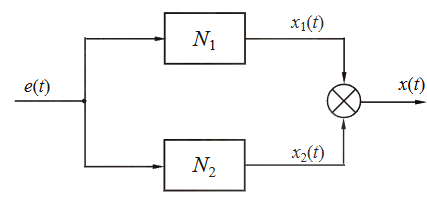
\includegraphics[width = .3\textwidth]{note/nonlinear system/figure/15.png}
\end{center}

此时：
\[
\begin{aligned}
x_1(t) &= N_1(A)A\sin\omega t \\
x_2(t) &= N_2(A)A\sin\omega t \\
x(t) &= x_1(t)+x_2(t) = \bigl(N_1(A)+N_2(A)\bigr)A\sin\omega t
\end{aligned}
\]

\[
N(A)=N_1(A)+N_2(A)
\]

\subsubsection{非线性串联叠加}

非线性的串联可以用以下的示意图表示：
\begin{center}
    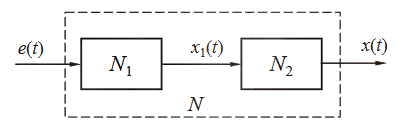
\includegraphics[width = .3\textwidth]{note/nonlinear system/figure/16.png}
\end{center}
由于非线性部分不满足叠加定理，故只能一步一步进行计算，先计算$N_1$模块的输出$x_1(t)$，再计算$N_2$模块的输出，如果还有模块则同理继续进行

\subsection{非线性系统的稳定性}

在讨论非线性系统的稳定性前，我们先由变增益线性系统的稳定性进行引入：

变增益线性系统示意图如下：
\begin{center}
    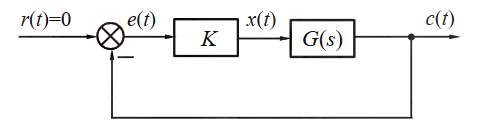
\includegraphics[width = .3\textwidth]{note/nonlinear system/figure/17.png}
\end{center}

设 $G(s)$ 的极点位于左半平面，闭环特征方程：
\[
1+KG(j\omega)=0
\quad \text{或} \quad
G(j\omega)=-\frac{1}{K}
\]

由 Nyquist 稳定判据可知：
\begin{itemize}
    \item 当 $\Gamma_G$ 曲线不包围 $\left(-\frac{1}{K},j0\right)$ 点时，即
    \[
    Z=P-2N=-2N=0
    \]
    时系统闭环稳定；

    \item 当 $\Gamma_G$ 曲线穿过 $\left(-\frac{1}{K},j0\right)$ 点时，系统临界稳定，将产生等幅震荡。

    \item 若设 $K$ 在一定范围内可变，即有 $K_1\le K\le K_2$，
    则 $\left(-\frac{1}{K},j0\right)$ 为复平面实轴上的一段直线，
    若 $\Gamma_G$ 曲线不包围该线段，则系统闭环稳定；
    当 $\Gamma_G$ 曲线包围该线段时，系统闭环不稳定。
\end{itemize}

故我们可以得出以下的非线性系统稳定性判据：

\begin{center}
    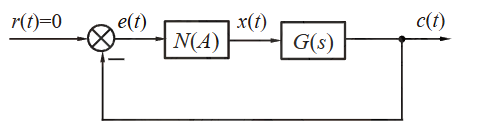
\includegraphics[width = .3\textwidth]{note/nonlinear system/figure/9.png}
\end{center}

假设：描述函数可以作为一个具有复变增益的比例环节；$G(s)$ 具有低通特性，故极点位于左半平面。

闭环特征方程：
\[
1+N(A)G(j\omega)=0
\quad \text{或} \quad
G(j\omega)=-\frac{1}{N(A)}
\]

即
\[
\begin{cases}
|G(j\omega)N(A)|=1 \\
\angle N(A)+\angle G(j\omega)=-180^\circ
\end{cases}
\]

推广的 Nyquist 稳定判据：
\begin{enumerate}
    \item 若线性环节的频率特性 $G(j\omega)$ 的轨迹不包围 $-\dfrac{1}{N(A)}$ 轨迹，如下图(a) 所示，则非线性系统是稳定的，并且 $G(j\omega)$ 离 $-\dfrac{1}{N(A)}$ 越远，系统稳定程度越高。

    \item 若 $G(j\omega)$ 轨迹包围 $-\dfrac{1}{N(A)}$ 轨迹，如下图(b)，则系统是不稳定的，系统将做发散运动。

    \item 若 $G(j\omega)$ 轨迹与 $-\dfrac{1}{N(A)}$ 轨迹有交点，如下图(c)所示，则系统中存在着等幅振荡，其振幅对应交点的振幅和频率。该等幅振荡可能是具有一定稳定性的等幅振荡，即自激振荡；也可能是不稳定的等幅振荡，即在一定条件下等幅振荡发散或收敛。
\end{enumerate}

\begin{center}
    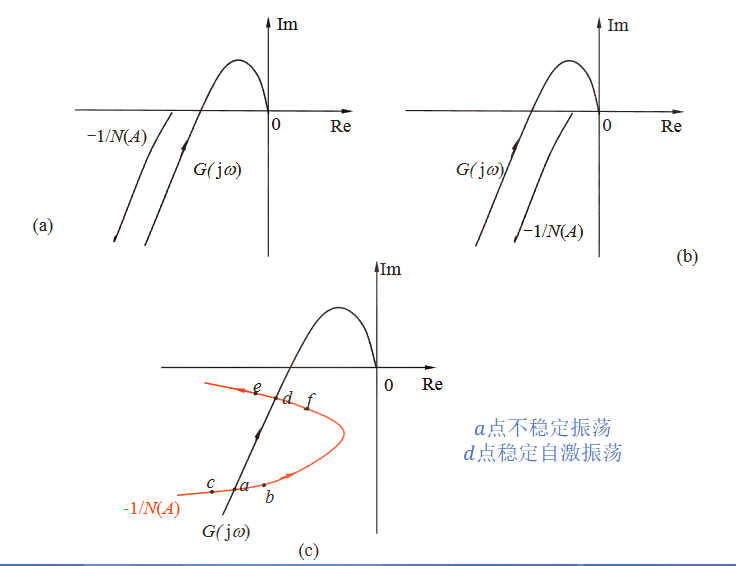
\includegraphics[width = .5\textwidth]{note/nonlinear system/figure/18.png}
\end{center}

从信号的角度分析自振荡产生的条件。在上面图示非线性系统中，若产生自激振荡，
则意味着系统中有一个正弦信号在流通，不妨设非线性环节的输入信号为
\[
e(t)=A\sin\omega t
\]

则非线性环节输出信号基波分量为
\[
x_1(t)=|N(A)|A\sin\!\bigl[\omega t+\angle N(A)\bigr]
\]

而线性部分的输出信号为
\[
c(t)=|G(j\omega)N(A)|A\sin\!\bigl[\omega t+\angle G(j\omega)+\angle N(A)\bigr]
\]

根据系统中存在自振荡的假设，$r(t)=0$，故
\[
e(t)=-c(t)
\]

即
\[
A\sin\omega t
=
-|G(j\omega)N(A)|A\sin\!\bigl[\omega t+\angle G(j\omega)+\angle N(A)\bigr]
\]

不妨以下图为例进行分析：
\begin{center}
    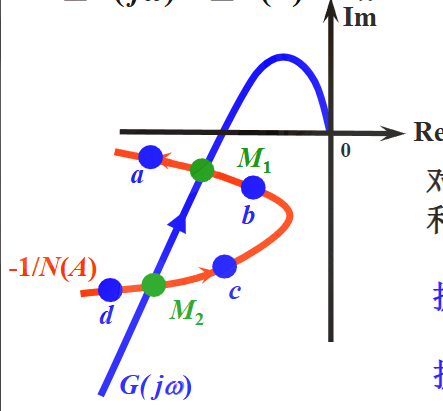
\includegraphics[width = .4\textwidth]{note/nonlinear system/figure/19.png}
\end{center}
其中$M_1$点是稳定的自激振荡点，$M_2$是不稳定的振荡点，对于稳定的自振荡，其振幅和频率是确定的，并可以测量得到。计算时：振幅可由 $-1/N(A)$ 曲线的自变量 $A$ 的大小来确定，振荡频率由 $G(j\omega)$ 曲线的自变量 $\omega$ 来确定。

\begin{example}
    非线性系统结构图如下，已知：
    \begin{center}
        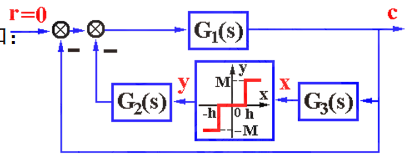
\includegraphics[width = .4\textwidth]{note/nonlinear system/figure/20.png}
    \end{center}
    \[
    \begin{cases}
    G_1(s)=\dfrac{1}{s(s+1)}, \qquad G_2(s)=\dfrac{K}{s} \\[6pt]
    N(A)=\dfrac{4M}{\pi A}\sqrt{1-\left(\dfrac{h}{A}\right)^2},
    \qquad A\ge h
    \end{cases}
    \]
    \begin{enumerate}
        \item $G_3(s) = 1$时，系统是否自振？确定使系统自振的$K$值的范围；求$K = 2$时的自振参数
        \item $G_3(s) = s$时，分析系统的稳定性
    \end{enumerate}
    \tcblower
    先将系统结构图化为典型结构
    \begin{itemize}
        \item 等效变换法：通过方框图法将系统化简：
        \begin{center}
            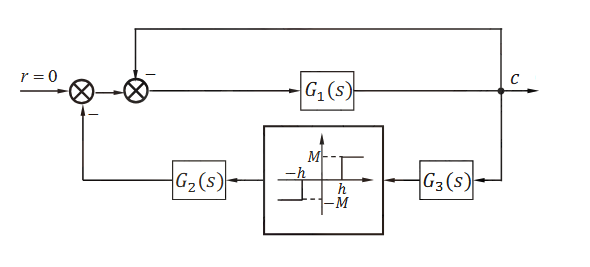
\includegraphics[width = .5\textwidth]{note/nonlinear system/figure/21.png} \\
            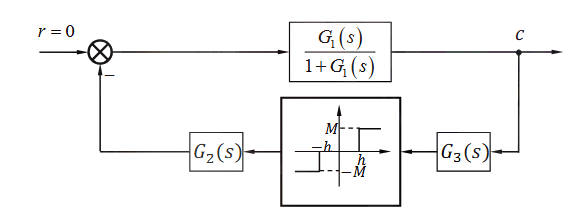
\includegraphics[width = .5\textwidth]{note/nonlinear system/figure/22.png}
        \end{center}
        故$G(s) = \frac{G_1}{1 + G_1} G_2 G_3$
        \item 特征方程法，采用类似线性系统的思想，给出系统的“闭环传递函数为”：
        \begin{align*}
            \Phi(s) = \frac{G_1}{1 + G_1 G_2 G_3 N + G_1}
        \end{align*}
        取出特征方程并化简可得：
        \begin{align*}
            &N\frac{G_1 G_2 G_3}{1 + G_1} = -1 \\
            &G(s) = \frac{G_1}{1 + G_1} G_2 G_3
        \end{align*}
    \end{itemize}
    \begin{enumerate}
        \item $G_3(s)=1$ 时
        \[
        \begin{aligned}
        G(s)
        &= \frac{G_1G_2G_3}{1+G_1} \\
        &= \frac{\dfrac{1}{s(s+1)}\cdot\dfrac{K}{s}\cdot 1}
        {1+\dfrac{1}{s(s+1)}} \\
        &= \frac{K}{s\left(s^2+s+1\right)}
        \end{aligned}
        \]

        \[
        -\frac{1}{N(A)}
        =
        \frac{-\pi A}{4M\sqrt{1-(h/A)^2}}
        =
        \frac{-\pi A^2}{4M\sqrt{A^2-h^2}}
        \]
        当$A \to h$时$\frac{-1}{N(A)} \to -\infty$，当$A\to \infty$时$\frac{-1}{N(A)} \to -\infty$

        由自振条件
        \[
        N(A)\cdot G(j\omega)=-1
        \]

        \[
        \frac{4M}{\pi A}\sqrt{1-\left(\frac{h}{A}\right)^2}
        \cdot
        \frac{K}{j\omega(1-\omega^2+j\omega)}
        =-1
        \]

        \[
        \begin{aligned}
        \frac{4MK}{\pi A}\sqrt{1-\left(\frac{h}{A}\right)^2}
        &= -j\omega(1-\omega^2+j\omega) \\
        &= \omega^2-j\omega(1-\omega^2)
        \end{aligned}
        \]
        观察实部和虚部可得：
        \[
        \begin{cases}
        \omega=1, \\[4pt]
        \dfrac{4K}{\pi A^2}\sqrt{A^2-1}=1\rightarrow\sqrt{A^2-1}=\dfrac{\pi A^2}{4K}.
        \end{cases}
        \]
        由第二条式子可以解得$A^2 = \frac{1 \pm \sqrt{1 - 4 (\pi / 4K)^2}}{2(\pi/4K)^2}$，所以有解的条件为：$K \ge \frac{\pi}{2}$，当$K= 2$时可以算出$A^2 = 5.25$或$1.1122$，故
        \[
        \begin{cases}
        A_1=2.29, \\
        A_2=1.055.
        \end{cases}
        \]
        由自激振荡的条件可以知道需要取大者，所以可以解得：
        \[
        \begin{cases}
        A=2.29, \\
        \omega=1.
        \end{cases}
        \]
        \item $G_3(s)=s$ 时
        \[
        \begin{aligned}
        G(s)
        &= \frac{G_1G_2G_3}{1+G_1} \\
        &= \frac{\dfrac{1}{s(s+1)}\cdot\dfrac{K}{s}\cdot s}
        {1+\dfrac{1}{s(s+1)}} \\
        &= \frac{K}{s^2+s+1}
        \end{aligned}
        \]
        画出图像如下，可以看出此时系统稳定
        \begin{center}
            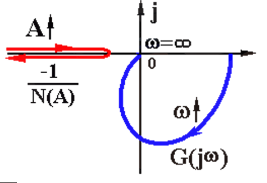
\includegraphics[width = .4\textwidth]{note/nonlinear system/figure/23.png}
        \end{center}
    \end{enumerate}
\end{example}

\section{相平面法}
\subsection{相平面法的基本概念}
相平面法是分析非线性系统稳定性的一个重要工具。对于一个二阶非线性系统，我们可以将其状态变量$x$和$\dot{x}$分别作为横轴和纵轴，在平面上描绘出系统的轨迹，这个平面就被称为相平面。在相平面上绘制出来的轨迹叫做相轨迹

我们可以给出相平面的一些性质如下：
\begin{property}[相平面的一些性质]
    \begin{enumerate}
        \item 相轨迹的斜率：$\frac{\mathrm{d}\dot{x}}{\mathrm{d}x}=\frac{-f(x,\dot{x})}{\dot{x}}$
        \item 相轨迹的就奇点（平衡点）：满足$\ddot{x} = \dot{x} = 0$的点，即相轨迹上的斜率不确定点，在$x$轴上，对于线性定常系统，原点是唯一的平衡点
        \item 相轨迹的运动方向：由斜率的符号可以确定相轨迹的运动方向
        \item 相轨迹通过横轴的方向：相轨迹以90°的角度穿过横轴
        \item 相轨迹的对称性：如果系统的函数$f(x,\dot{x})$是$x$的奇函数，那么相轨迹关于$\dot{x}$轴对称；如果$f(x,\dot{x})$是$\dot{x}$的偶函数，那么相轨迹关于$x$轴对称。
    \end{enumerate}
\end{property}

\subsection{相轨迹的绘制}

\subsubsection{解析法}
解析法是通过求解系统的微分方程来得到相轨迹的表达式，从而绘制出相轨迹，我们有以下两种方法：
\begin{enumerate}
    \item 直接积分法：通过将系统的微分方程进行积分，得到相轨迹的表达式，从而绘制出相轨迹。
    \item 消去时间变量$t$：通过将系统的微分方程中的时间变量$t$消去，得到一个关于$x$和$\dot{x}$的方程，从而绘制出相轨迹。
\end{enumerate}

\subsubsection{等倾线法}
对于二阶系统
\[
\ddot{x}+f(x,\dot{x})=0,
\]
其斜率方程为：
\[
\frac{d\dot{x}}{dx}=-\frac{f(x,\dot{x})}{\dot{x}}
\]

该方程给出了相轨迹在相平面上任一点 $(x,\dot{x})$ 处切线的斜率。取相轨迹切线的斜率为某一常数 $\alpha$，得：
\[
\alpha=\frac{d\dot{x}}{dx}=-\frac{f(x,\dot{x})}{\dot{x}}
\]

也就是说，相平面上满足该方程的点 $(x,\dot{x})$，其所对应的相轨迹在该点处切线的斜率为 $\alpha$。如果 $\dot{x}\neq 0$，则：
\[
\alpha\dot{x}+f(x,\dot{x})=0
\]

该方程称为二阶系统的等倾线方程。

\begin{itemize}
    \item 二阶系统的等倾线方程可将系统方程 $\ddot{x}+f(x,\dot{x})=0$ 中 $\ddot{x}$ 替换为 $\alpha\dot{x}$ 得到。
    \item 根据等倾线方程，可在相平面的各条相轨迹上求出具有同一斜率的点 $(x,\dot{x})$，将这些点连接起来，由此得到的等斜率轨迹亦称为等倾线。
\end{itemize}

对于二阶线性系统，
\[
\ddot{x}+a\dot{x}+bx=0
\]

其等倾线为直线，其方程为：
\[
\dot{x}=-\frac{b}{a+\alpha}x
\]

其中 $\alpha$ 为相轨迹切线的斜率，而该等倾线的斜率为：
\[
k=-\frac{b}{a+\alpha}
\]

考虑一类等倾线：等倾线的斜率与相轨迹切线斜率相等。这类等倾线也是相轨迹。
\[
k=-\frac{b}{a+k}
\]

\[
k^2+ak+b=0
\]

\begin{itemize}
    \item 特殊等倾线的斜率是系统的极点。
    \item 具有复数极点的二阶线性系统不存在这样的特殊等倾线。
\end{itemize}

当 $b<0$ 时，系统的两个极点为：
\[
s_1=-\frac{a+\sqrt{a^2-4b}}{2}<0,
\qquad
s_2=-\frac{a-\sqrt{a^2-4b}}{2}>0
\]

\subsubsection{线性二阶系统的相轨迹}

我们研究以下这种系统的不同情况：
\begin{align*}
    \ddot{x} + 2 \xi \omega_n \dot{x} + \omega_n^2 x = 0
\end{align*}

\begin{enumerate}
    \item $0<\xi<1$时，系统有两个实部为负的共轭复根，系统的奇点为稳定焦点，如下图所示：
    \begin{center}
        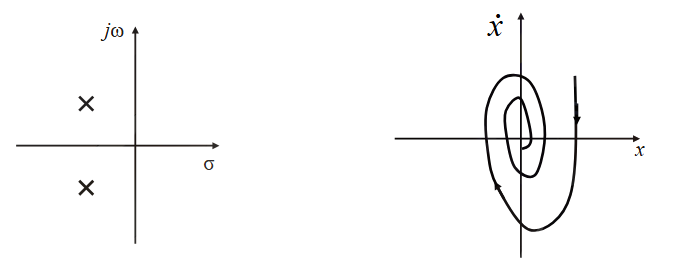
\includegraphics[width = .5\textwidth]{note/nonlinear system/figure/24.png}
    \end{center}
    \item $-1<\xi<0$时，系统有两个实部为正的共轭复根，系统的奇点为不稳定焦点，如下图所示：
    \begin{center}
        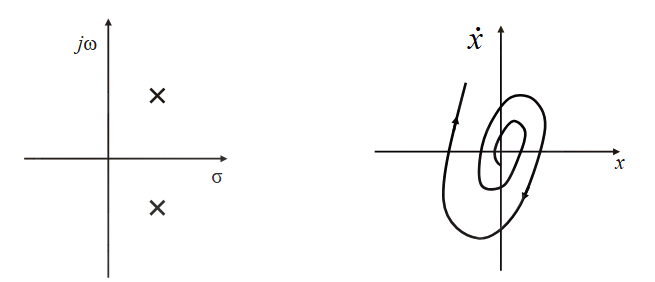
\includegraphics[width = .5\textwidth]{note/nonlinear system/figure/25.png}
    \end{center}
    \item $\xi>1$时，系统有两个负实根，相轨迹中有两条特殊等倾线，系统的奇点为稳定节点，如下图所示：
    \begin{center}
        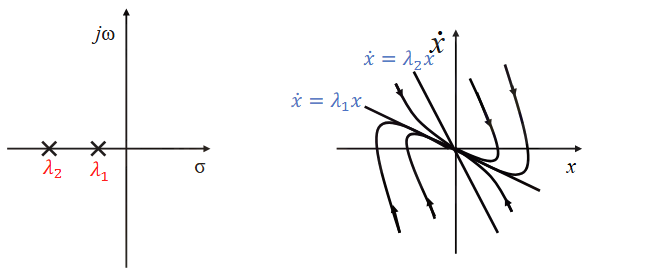
\includegraphics[width = .5\textwidth]{note/nonlinear system/figure/26.png}
    \end{center}
    \item $\xi<-1$时，系统有两个正实根，相轨迹中有两条特殊等倾线，系统的奇点为不稳定节点，如下图所示：
    \begin{center}
        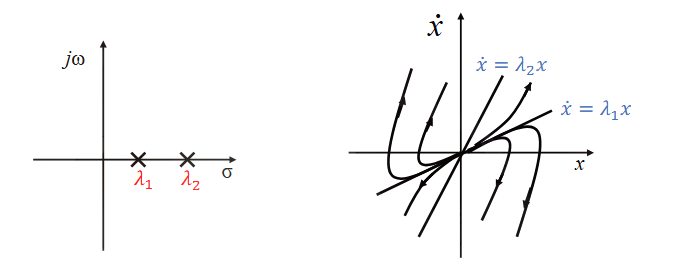
\includegraphics[width = .5\textwidth]{note/nonlinear system/figure/27.png}
    \end{center}
    \item $\xi = 0$时，系统有两个实部为零的共轭复根，系统的奇点为中心点，相轨迹为以奇点为中心的同心椭圆，如下图所示：
    \begin{center}
        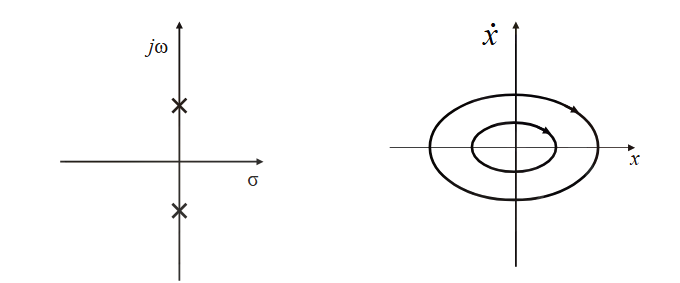
\includegraphics[width = .5\textwidth]{note/nonlinear system/figure/28.png}
    \end{center}
    \item 考虑另一个二阶线性系统：$\ddot{x} + 2\xi \omega_n \dot{x} - \omega_n^2 x = 0$，此系统含有两个异号实根，相轨迹有两条特殊等倾线，系统的奇点为鞍点，如下图所示：
    \begin{center}
        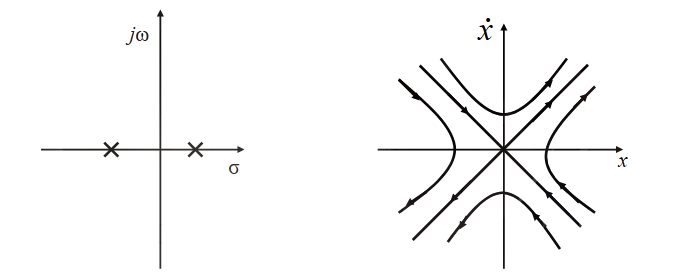
\includegraphics[width = .5\textwidth]{note/nonlinear system/figure/29.png}
    \end{center}
\end{enumerate}

以上的六种情况可以总结为以下这一张图：
\begin{center}
    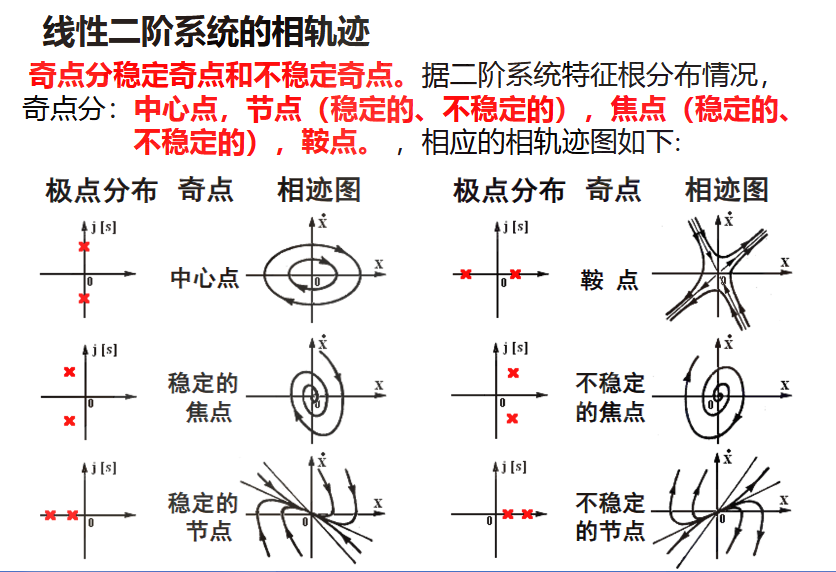
\includegraphics[width = .6\textwidth]{note/nonlinear system/figure/30.png}
\end{center}

\subsubsection{非线性系统的相轨迹}

对于非线性系统，平衡状态和平衡状态附近系统的运动形式以及极限环的存在
制约着整个系统的运动特性。对于非线性系统的各个平衡点，若描述非线性过程的
非线性函数解析时，可以通过平衡点处的线性化方程，基于线性系统特征根的分布，
确定奇点的类型，进而确定平衡点附近相轨迹的运动形式。

\begin{enumerate}
    \item 若$f(x,\dot{x})$解析，则我们可以将方程$\ddot{x} + f(x,\dot{x}) = 0$在奇点$(x_0,\dot{x}_0)$处展开：
    \[
    \Delta \ddot{x}
    = - \left. \frac{\partial f(x,\dot{x})}{\partial x} \right|_{\substack{x=x_0\\ \dot{x}=\dot{x}_0}} \Delta x
    - \left. \frac{\partial f(x,\dot{x})}{\partial \dot{x}} \right|_{\substack{x=x_0\\ \dot{x}=\dot{x}_0}} \Delta \dot{x}
    \]
    此时微分方程就可以近似写为一个二阶线性方程：
    \[
         \ddot{x}
     + \left. \frac{\partial f(x,\dot{x})}{\partial x} \right|_{\substack{x=x_0\\ \dot{x}=\dot{x}_0}}  x
    + \left. \frac{\partial f(x,\dot{x})}{\partial \dot{x}} \right|_{\substack{x=x_0\\ \dot{x}=\dot{x}_0}}  \dot{x} = 0
    \]
    \item 如果$f(x,\dot{x})$不解析，可以根据非线性特性将相平面划分成若干区域
    \begin{itemize}
        \item 在各区域内，非线性方程$f(x,\dot{x})$可满足解析条件或可以表示为线性微分方程
        \item 若某区域内非线性方程可线性化，奇点类型即决定该区域系统运动的形态
        \item 若对应奇点位于本区域内，称为实奇点，若对应奇点位于其他区域，称为虚奇点
    \end{itemize}
    \item 当非线性系统存在多个奇点时，奇点类型只决定奇点附近相轨迹的运动形式。
    \item 整个系统的相轨迹，特别是离奇点较远的部分，还取决于多个奇点的共同作用。
    \item 有时会产生特殊的相轨迹，将相平面划分为具有不同运动特点的多个区域。这种特殊的相轨迹称为奇线。
    \item 最常见的奇线是极限环。极限环把相平面的某个区域划分为内部平面和外部平面部分。
    \begin{itemize}
        \item 极限环是非线性系统的特有现象，表示系统稳态运动的、孤立的封闭曲线。
        \item 把相平面划分为具有不同运动特点的各个区域。
        \item 收敛于该极限环，则极限环称为稳定极限环。系统呈现稳定的自振。
        \item 一些复杂的非线性控制系统可能出现两个或两个以上极限环。
        \item 该非线性系统的工作状态，不仅取决于初始条件，也取决于扰动大小。
        \item 只有稳定的极限环才能在实验中被观察到。不稳定或半稳定的极限环无法在实验中观察到
    \end{itemize}
    \item 常见非线性特性多数可用分段直线来表示，或者本身就是分段线性的。
    \item 对于含有这些非线性特性的一大类非线性系统，由于不满足解析条件，无法采用小扰动线性化方法。
    \item 根据非线性的分段特点，将相平面分成若干区域进行研究，可使非线性微分方程在各个区域表现为线性微分方程，再应用线性系统的相平面分析方法，则问题将迎刃而解。
    \item 这一类非线性特性曲线的折线的各转折点，构成了相平面区域的分界线，称为\textcolor{red}{开关线}。
\end{enumerate}

\begin{example}
    系统如下，已知
\[
\begin{cases}
c(0)=0,\\
r(t)=4\times 1(t),
\end{cases}
\]
确定开关线方程、奇点位置和类型，绘制相轨迹 $(e,\dot{e})$ 图。
\begin{center}
    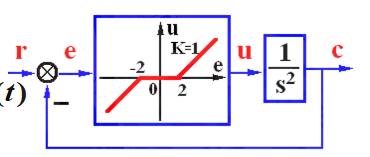
\includegraphics[width = .5\textwidth]{note/nonlinear system/figure/31.png}
\end{center}
\tcblower
线性部分：
\[
\frac{C(s)}{U(s)}=\frac{1}{s^2}
\quad \Rightarrow \quad
\ddot{c}(t)=u(t)
\]

非线性部分：
\[
u=
\begin{cases}
0, & |e|\leq 2 \quad (\mathrm{I})\\
e-2, & e>2 \quad (\mathrm{II})\\
e+2, & e<-2 \quad (\mathrm{III})
\end{cases}
\]

开关线方程：
\[
\begin{cases}
e=2,\\
e=-2.
\end{cases}
\]

综合点：
\[
e=r-c=4-c
\]
\[
\begin{cases}
c=4-e,\\
\dot{c}=-\dot{e},\\
\ddot{c}=-\ddot{e}.
\end{cases}
\]

因此
\[
\ddot{e}
=-\ddot{c}
=-u
=
\begin{cases}
0, & |e|\leq 2 \quad (\mathrm{I})\\
2-e, & e>2 \quad (\mathrm{II})\\
-2-e, & e<-2 \quad (\mathrm{III})
\end{cases}
\]
因此可以画出以下这个表：
\[
\begin{array}{c|c|c|c|c|c}
\text{区域} & \text{运动方程} & \text{奇点} & \text{特征方程} & \text{极点} & \text{奇点性质} \\
\hline
\mathrm{I} & \ddot{e}=0 & \dot{e}=0 & s^2=0 & s=0 & \\
\mathrm{II} & \ddot{e}+e-2=0 & (2,0) & s^2+1=0 & s=\pm j & \text{中心点} \\
\mathrm{III} & \ddot{e}+e+2=0 & (-2,0) & s^2+1=0 & s=\pm j & \text{中心点}
\end{array}
\]
所以相轨迹为：
\[
\begin{cases}
(\mathrm{I}) \quad \ddot{e}=0,\quad \dot{e}=C, \quad \text{水平线},\\
(\mathrm{II}) \quad \text{以 } (2,0) \text{ 为中心的圆},\\
(\mathrm{III}) \quad \text{以 } (-2,0) \text{ 为中心的圆}.
\end{cases}
\]
画出相轨迹如下：
\begin{center}
    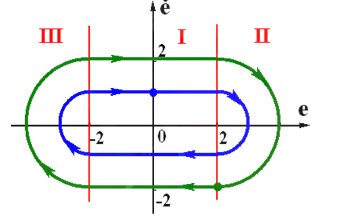
\includegraphics[width = .4\textwidth]{note/nonlinear system/figure/32.png}
\end{center}
\end{example}

\begin{example}
    系统如下，在 $(c,\dot{c})$ 平面上分析系统的自由响应运动。
    \begin{center}
        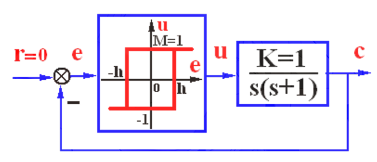
\includegraphics[width = .4\textwidth]{note/nonlinear system/figure/33.png}
    \end{center}
    \tcblower
线性部分：
\[
\frac{C(s)}{U(s)}=\frac{1}{s^2+s}
\]

\[
\ddot{c}+\dot{c}=u
\]

非线性部分：
\[
u=
\begin{cases}
1,
&
\begin{cases}
e>h,\\
e>-h,\ \dot{e}<0,
\end{cases}
\\[6pt]
-1,
&
\begin{cases}
e<-h,\\
e<h,\ \dot{e}>0.
\end{cases}
\end{cases}
\]

比较点：
\[
e=r-c
\]

自由响应时 $r=0$，故
\[
e=-c,\qquad \dot{e}=-\dot{c}
\]

整理：
\[
\ddot{c}+\dot{c}=u=
\begin{cases}
1,
&
\begin{cases}
c<-h,\\
c<h,\ \dot{c}>0,
\end{cases}
\\[6pt]
-1,
&
\begin{cases}
c>h,\\
c>-h,\ \dot{c}<0.
\end{cases}
\end{cases}
\]
所以可以画出开关线如下：
\begin{center}
    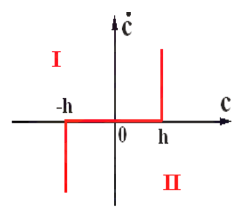
\includegraphics[width = .4\textwidth]{note/nonlinear system/figure/34.png}
\end{center}
\[
(\mathrm{I})\quad
\ddot{c}
=
\dot{c}\frac{d\dot{c}}{dc}
=
\alpha \dot{c}
=
1-\dot{c}
\qquad
\text{等倾斜线 }
\dot{c}=\frac{1}{1+\alpha}
\]

\[
(\mathrm{II})\quad
\ddot{c}
=
\dot{c}\frac{d\dot{c}}{dc}
=
\alpha \dot{c}
=
-1-\dot{c}
\qquad
\text{等倾斜线 }
\dot{c}=\frac{-1}{1+\alpha}
\]
根据上面的式子可以给出以下这个表：
\[
\begin{array}{cc|cccccccc}
\multicolumn{2}{c|}{\alpha}
& -\frac{1}{2} & -\frac{1}{3} & 0 & 1 & \infty & -3 & -2 & -\frac{3}{2} \\
\hline
\mathrm{I} & \frac{1}{1+\alpha}
& 2 & \frac{3}{2} & 1 & \frac{1}{2} & 0 & -\frac{1}{2} & -1 & -2 \\
\mathrm{II} & -\frac{1}{1+\alpha}
& -2 & -\frac{3}{2} & -1 & -\frac{1}{2} & 0 & \frac{1}{2} & 1 & 2
\end{array}
\]
所以可以画出系统的相轨迹如下：
\begin{center}
    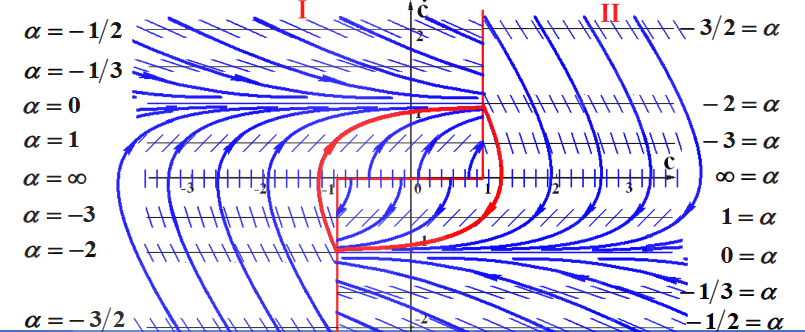
\includegraphics[width = .6\textwidth]{note/nonlinear system/figure/35.png}
\end{center}
\end{example}


\end{document}
